% Options for packages loaded elsewhere
% Options for packages loaded elsewhere
\PassOptionsToPackage{unicode}{hyperref}
\PassOptionsToPackage{hyphens}{url}
\PassOptionsToPackage{dvipsnames,svgnames,x11names}{xcolor}
%
\documentclass[
  spanish,
  letterpaper,
  DIV=11,
  numbers=noendperiod]{scrreprt}
\usepackage{xcolor}
\usepackage{amsmath,amssymb}
\setcounter{secnumdepth}{5}
\usepackage{iftex}
\ifPDFTeX
  \usepackage[T1]{fontenc}
  \usepackage[utf8]{inputenc}
  \usepackage{textcomp} % provide euro and other symbols
\else % if luatex or xetex
  \usepackage{unicode-math} % this also loads fontspec
  \defaultfontfeatures{Scale=MatchLowercase}
  \defaultfontfeatures[\rmfamily]{Ligatures=TeX,Scale=1}
\fi
\usepackage{lmodern}
\ifPDFTeX\else
  % xetex/luatex font selection
\fi
% Use upquote if available, for straight quotes in verbatim environments
\IfFileExists{upquote.sty}{\usepackage{upquote}}{}
\IfFileExists{microtype.sty}{% use microtype if available
  \usepackage[]{microtype}
  \UseMicrotypeSet[protrusion]{basicmath} % disable protrusion for tt fonts
}{}
\makeatletter
\@ifundefined{KOMAClassName}{% if non-KOMA class
  \IfFileExists{parskip.sty}{%
    \usepackage{parskip}
  }{% else
    \setlength{\parindent}{0pt}
    \setlength{\parskip}{6pt plus 2pt minus 1pt}}
}{% if KOMA class
  \KOMAoptions{parskip=half}}
\makeatother
% Make \paragraph and \subparagraph free-standing
\makeatletter
\ifx\paragraph\undefined\else
  \let\oldparagraph\paragraph
  \renewcommand{\paragraph}{
    \@ifstar
      \xxxParagraphStar
      \xxxParagraphNoStar
  }
  \newcommand{\xxxParagraphStar}[1]{\oldparagraph*{#1}\mbox{}}
  \newcommand{\xxxParagraphNoStar}[1]{\oldparagraph{#1}\mbox{}}
\fi
\ifx\subparagraph\undefined\else
  \let\oldsubparagraph\subparagraph
  \renewcommand{\subparagraph}{
    \@ifstar
      \xxxSubParagraphStar
      \xxxSubParagraphNoStar
  }
  \newcommand{\xxxSubParagraphStar}[1]{\oldsubparagraph*{#1}\mbox{}}
  \newcommand{\xxxSubParagraphNoStar}[1]{\oldsubparagraph{#1}\mbox{}}
\fi
\makeatother


\usepackage{longtable,booktabs,array}
\usepackage{calc} % for calculating minipage widths
% Correct order of tables after \paragraph or \subparagraph
\usepackage{etoolbox}
\makeatletter
\patchcmd\longtable{\par}{\if@noskipsec\mbox{}\fi\par}{}{}
\makeatother
% Allow footnotes in longtable head/foot
\IfFileExists{footnotehyper.sty}{\usepackage{footnotehyper}}{\usepackage{footnote}}
\makesavenoteenv{longtable}
\usepackage{graphicx}
\makeatletter
\newsavebox\pandoc@box
\newcommand*\pandocbounded[1]{% scales image to fit in text height/width
  \sbox\pandoc@box{#1}%
  \Gscale@div\@tempa{\textheight}{\dimexpr\ht\pandoc@box+\dp\pandoc@box\relax}%
  \Gscale@div\@tempb{\linewidth}{\wd\pandoc@box}%
  \ifdim\@tempb\p@<\@tempa\p@\let\@tempa\@tempb\fi% select the smaller of both
  \ifdim\@tempa\p@<\p@\scalebox{\@tempa}{\usebox\pandoc@box}%
  \else\usebox{\pandoc@box}%
  \fi%
}
% Set default figure placement to htbp
\def\fps@figure{htbp}
\makeatother



\ifLuaTeX
\usepackage[bidi=basic]{babel}
\else
\usepackage[bidi=default]{babel}
\fi
% get rid of language-specific shorthands (see #6817):
\let\LanguageShortHands\languageshorthands
\def\languageshorthands#1{}


\setlength{\emergencystretch}{3em} % prevent overfull lines

\providecommand{\tightlist}{%
  \setlength{\itemsep}{0pt}\setlength{\parskip}{0pt}}



 


\KOMAoption{captions}{tableheading}
\makeatletter
\@ifpackageloaded{tcolorbox}{}{\usepackage[skins,breakable]{tcolorbox}}
\@ifpackageloaded{fontawesome5}{}{\usepackage{fontawesome5}}
\definecolor{quarto-callout-color}{HTML}{909090}
\definecolor{quarto-callout-note-color}{HTML}{0758E5}
\definecolor{quarto-callout-important-color}{HTML}{CC1914}
\definecolor{quarto-callout-warning-color}{HTML}{EB9113}
\definecolor{quarto-callout-tip-color}{HTML}{00A047}
\definecolor{quarto-callout-caution-color}{HTML}{FC5300}
\definecolor{quarto-callout-color-frame}{HTML}{acacac}
\definecolor{quarto-callout-note-color-frame}{HTML}{4582ec}
\definecolor{quarto-callout-important-color-frame}{HTML}{d9534f}
\definecolor{quarto-callout-warning-color-frame}{HTML}{f0ad4e}
\definecolor{quarto-callout-tip-color-frame}{HTML}{02b875}
\definecolor{quarto-callout-caution-color-frame}{HTML}{fd7e14}
\makeatother
\makeatletter
\@ifpackageloaded{bookmark}{}{\usepackage{bookmark}}
\makeatother
\makeatletter
\@ifpackageloaded{caption}{}{\usepackage{caption}}
\AtBeginDocument{%
\ifdefined\contentsname
  \renewcommand*\contentsname{Tabla de contenidos}
\else
  \newcommand\contentsname{Tabla de contenidos}
\fi
\ifdefined\listfigurename
  \renewcommand*\listfigurename{Listado de Figuras}
\else
  \newcommand\listfigurename{Listado de Figuras}
\fi
\ifdefined\listtablename
  \renewcommand*\listtablename{Listado de Tablas}
\else
  \newcommand\listtablename{Listado de Tablas}
\fi
\ifdefined\figurename
  \renewcommand*\figurename{Figura}
\else
  \newcommand\figurename{Figura}
\fi
\ifdefined\tablename
  \renewcommand*\tablename{Tabla}
\else
  \newcommand\tablename{Tabla}
\fi
}
\@ifpackageloaded{float}{}{\usepackage{float}}
\floatstyle{ruled}
\@ifundefined{c@chapter}{\newfloat{codelisting}{h}{lop}}{\newfloat{codelisting}{h}{lop}[chapter]}
\floatname{codelisting}{Listado}
\newcommand*\listoflistings{\listof{codelisting}{Listado de Listados}}
\makeatother
\makeatletter
\makeatother
\makeatletter
\@ifpackageloaded{caption}{}{\usepackage{caption}}
\@ifpackageloaded{subcaption}{}{\usepackage{subcaption}}
\makeatother
\usepackage{bookmark}
\IfFileExists{xurl.sty}{\usepackage{xurl}}{} % add URL line breaks if available
\urlstyle{same}
\hypersetup{
  pdftitle={Notas de clase Business Analytics},
  pdfauthor={Daniel Parra},
  pdflang={es},
  colorlinks=true,
  linkcolor={blue},
  filecolor={Maroon},
  citecolor={Blue},
  urlcolor={Blue},
  pdfcreator={LaTeX via pandoc}}


\title{Notas de clase Business Analytics}
\author{Daniel Parra}
\date{Invalid Date}
\begin{document}
\maketitle

\renewcommand*\contentsname{Tabla de contenidos}
{
\hypersetup{linkcolor=}
\setcounter{tocdepth}{2}
\tableofcontents
}

\bookmarksetup{startatroot}

\chapter*{Bienvenidos}\label{bienvenidos}
\addcontentsline{toc}{chapter}{Bienvenidos}

\markboth{Bienvenidos}{Bienvenidos}

Este libro ha sido creado con el propósito de ofrecer un resumen claro y
conciso de los conceptos clave de las clases de Business Analytics para
los posgrados de administración de la Pontificia Universidad Javeriana.
Es un complemento diseñado para reforzar el aprendizaje en clase, pero
no pretende reemplazar la experiencia educativa que estas ofrecen.

Parte del texto en estas notas de clase ha sido elaborado con ayuda de
inteligencia artificial (ChatGPT), combinando apuntes propios y
referencias de diversos libros. Las ilustraciones, inspiradas en el
libro ``Math with Bad Drawings'' de Ben Orlin, también han sido
generadas utilizando inteligencia artificial.

© 2025 Pontificia Universidad Javeriana. Este libro está licenciado bajo
una licencia CC BY 4.0.

\bookmarksetup{startatroot}

\chapter{Introducción: Descubriendo la Analítica de
Datos}\label{introducciuxf3n-descubriendo-la-analuxedtica-de-datos}

Imagina que trabajas en una empresa que debe decidir qué producto lanzar
o qué precio poner a sus artículos. ¿Cómo tomas estas decisiones?
Antiguamente, las decisiones se tomaban según la intuición del jefe
(\textbf{HiPPO}, la persona mejor pagada en la organización), pero
actualmente contamos con algo mejor: la analítica de datos.

\section{¿Qué es la Analítica de Datos para
Negocios?}\label{quuxe9-es-la-analuxedtica-de-datos-para-negocios}

La analítica de datos es la aplicación de herramientas tecnológicas y
estadísticas para analizar información relevante y apoyar la toma de
decisiones en una organización.

Los datos, sin embargo, no son suficientes por sí solos. Necesitamos
interpretarlos de manera efectiva para contar historias convincentes que
permitan tomar decisiones informadas.

\section{¿Qué tipo de preguntas podemos responder con la
analítica?}\label{quuxe9-tipo-de-preguntas-podemos-responder-con-la-analuxedtica}

La analítica de negocios nos permite responder preguntas prácticas,
como:

\begin{itemize}
\tightlist
\item
  ¿Quiénes son mis clientes?
\item
  ¿Qué campaña de marketing es más efectiva?
\item
  ¿Cuál sería el efecto de cambiar los precios?
\item
  ¿Cómo predecir la demanda de un producto?
\end{itemize}

\section{Tipos de Analítica}\label{tipos-de-analuxedtica}

Hay tres tipos principales de analítica:

\subsection{Analítica Descriptiva}\label{analuxedtica-descriptiva}

Describe la situación actual mediante visualizaciones y estadísticas
básicas.

\textbf{Ejemplos:}

\begin{itemize}
\tightlist
\item
  ¿Han crecido las ventas este año?
\item
  ¿Qué región vende menos?
\end{itemize}

\subsection{Analítica Predictiva}\label{analuxedtica-predictiva}

Predice qué sucederá, aprovechando correlaciones entre variables. Aquí
no es necesaria la causalidad, sino una relación estadística sólida.

\textbf{Ejemplos:}

\begin{itemize}
\tightlist
\item
  ¿Cuál es la probabilidad de que un cliente deje de comprar?
\item
  ¿Qué tan probable es que una transacción sea fraudulenta?
\end{itemize}

\subsection{Analítica Prescriptiva}\label{analuxedtica-prescriptiva}

Sugiere decisiones óptimas, enfocándose en relaciones causales y,
frecuentemente, utilizando experimentos.

\textbf{Ejemplos:}

\begin{itemize}
\tightlist
\item
  ¿Subir el precio incrementará las ganancias?
\item
  ¿Qué diseño de página web aumentará las ventas?
\end{itemize}

\section{La cadena de valor en Business
Analytics}\label{la-cadena-de-valor-en-business-analytics}

La analítica de negocios incluye:

\begin{itemize}
\tightlist
\item
  \textbf{Recolección y organización de datos:} Crear bases de datos
  (SQL, Power BI).
\item
  \textbf{Análisis de datos:} Usar herramientas como R, Excel o Python
  para análisis estratégicos.
\item
  \textbf{Comunicación de resultados:} Presentar hallazgos en reportes y
  visualizaciones (PowerPoint, Tableau, Quarto).
\end{itemize}

\bookmarksetup{startatroot}

\chapter{Fundamentos de Variables y Visualización de
Datos}\label{fundamentos-de-variables-y-visualizaciuxf3n-de-datos}

\section{Introducción a Variables y
Datos}\label{introducciuxf3n-a-variables-y-datos}

Antes de manipular o graficar, es importante entender qué son los datos
y las variables.

\begin{tcolorbox}[enhanced jigsaw, toptitle=1mm, opacitybacktitle=0.6, leftrule=.75mm, arc=.35mm, title=\textcolor{quarto-callout-note-color}{\faInfo}\hspace{0.5em}{Definiciones clave}, colback=white, bottomrule=.15mm, colbacktitle=quarto-callout-note-color!10!white, opacityback=0, bottomtitle=1mm, breakable, rightrule=.15mm, coltitle=black, left=2mm, titlerule=0mm, colframe=quarto-callout-note-color-frame, toprule=.15mm]

\begin{itemize}
\tightlist
\item
  \textbf{Variable:} Característica que puede cambiar entre
  observaciones (ej. género, ventas, PIB).\\
\item
  \textbf{Datos:} Conjunto de observaciones (filas) con valores para
  esas variables (columnas).
\end{itemize}

\end{tcolorbox}

\subsection{Tipos de variables}\label{tipos-de-variables}

Las variables se clasifican en dos grandes categorías según su
naturaleza:

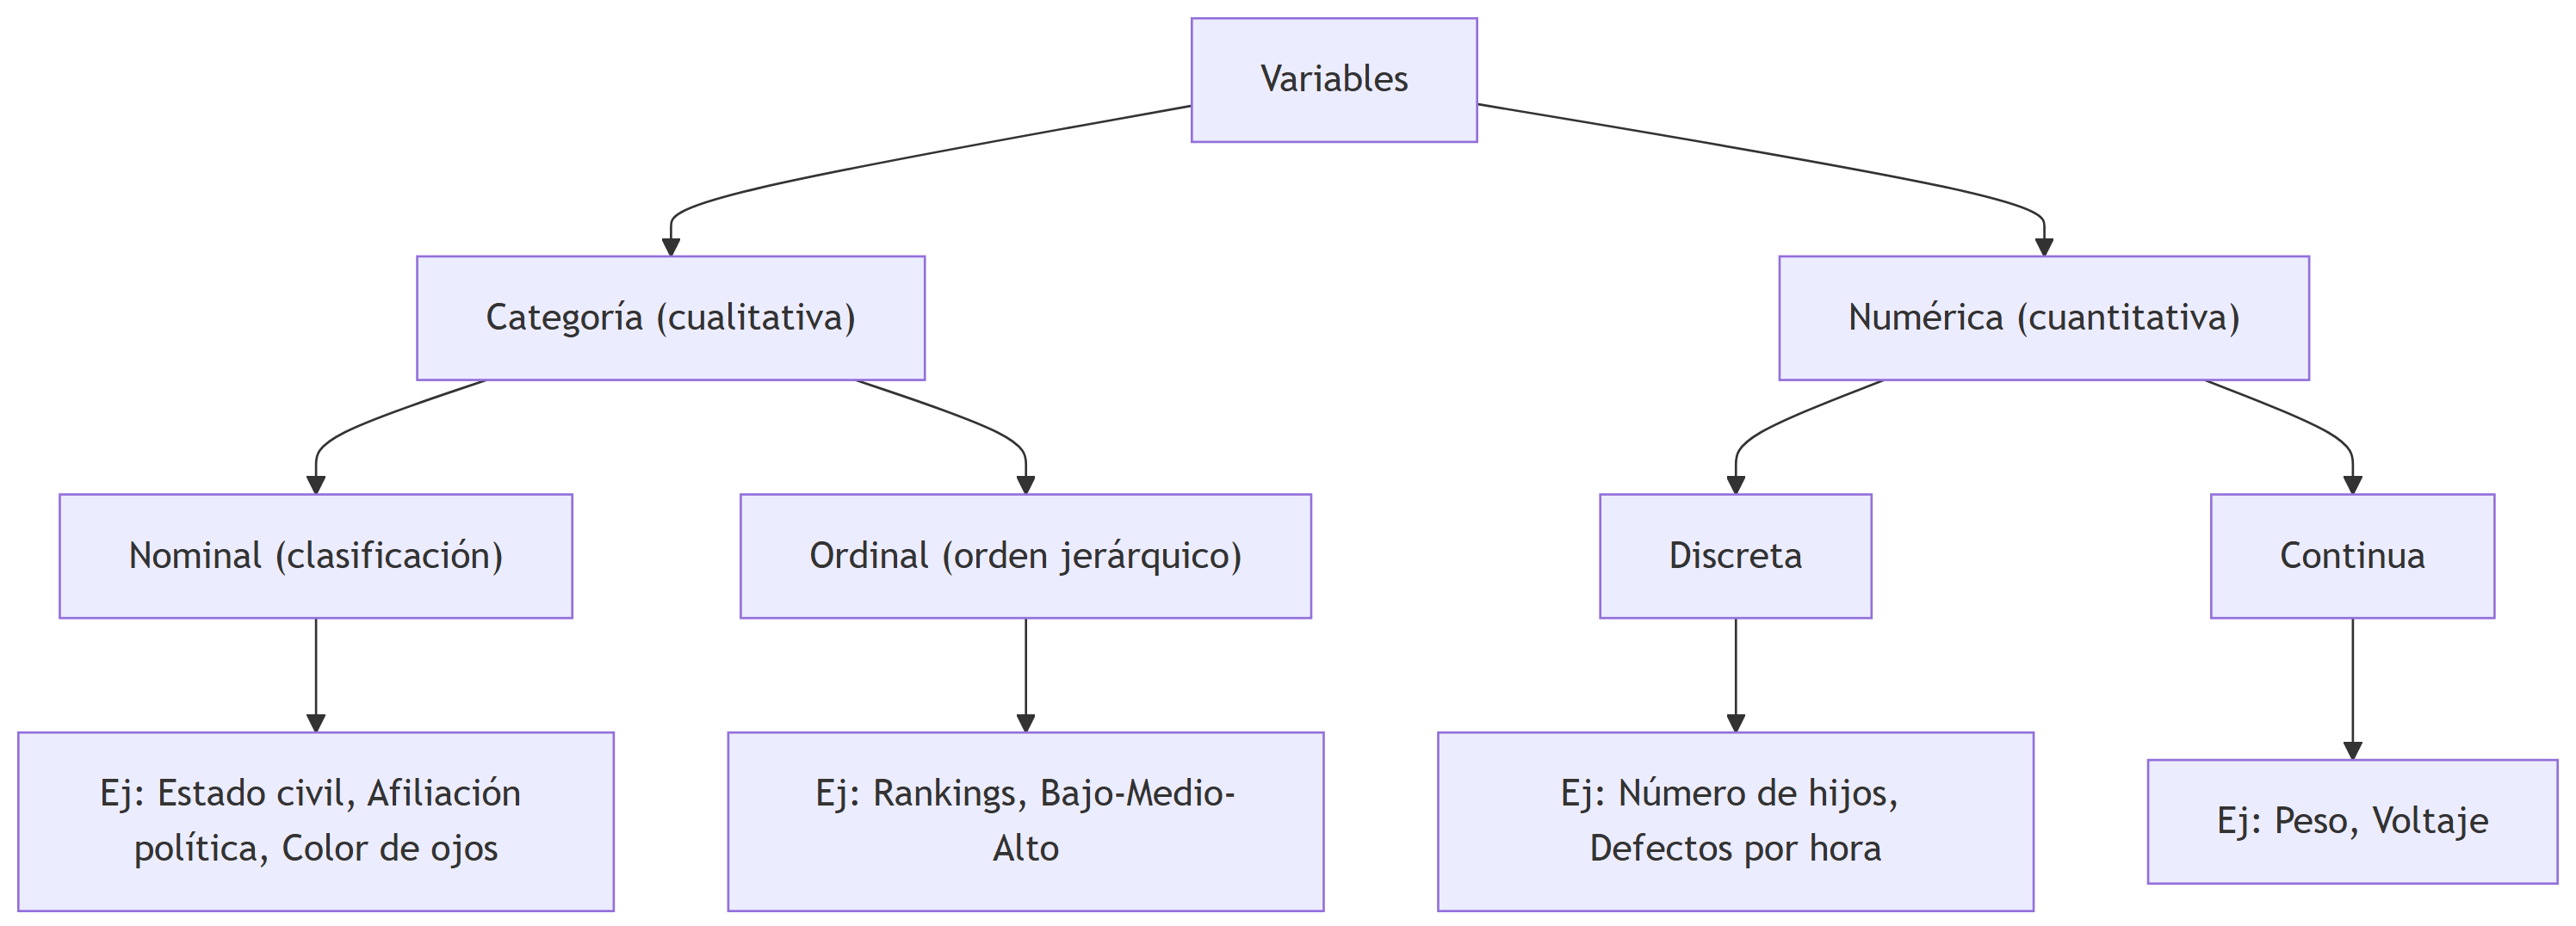
\includegraphics[width=11.72in,height=4.23in]{capitulo2_files/figure-latex/mermaid-figure-1.png}

Clasificación de Variables

Entender el tipo de variable es clave porque:

\begin{itemize}
\tightlist
\item
  \textbf{Define el resumen estadístico adecuado:} No calculamos una
  media de colores de ojos.\\
\item
  \textbf{Determina el gráfico apropiado:} Un histograma para variables
  numéricas, un gráfico de barras para categorías.\\
\item
  \textbf{Evita errores de interpretación:} Un ordinal tratado como
  numérico puede dar conclusiones equivocadas.
\end{itemize}

Ejemplos de tipos de variables:

\begin{longtable}[]{@{}
  >{\raggedright\arraybackslash}p{(\linewidth - 4\tabcolsep) * \real{0.4924}}
  >{\raggedright\arraybackslash}p{(\linewidth - 4\tabcolsep) * \real{0.3258}}
  >{\raggedright\arraybackslash}p{(\linewidth - 4\tabcolsep) * \real{0.1818}}@{}}
\caption{Ejemplo: Tipos de Variables en una
Encuesta}\label{tbl-ejemplos}\tabularnewline
\toprule\noalign{}
\begin{minipage}[b]{\linewidth}\raggedright
Pregunta
\end{minipage} & \begin{minipage}[b]{\linewidth}\raggedright
Respuesta
\end{minipage} & \begin{minipage}[b]{\linewidth}\raggedright
Tipo de Variable
\end{minipage} \\
\midrule\noalign{}
\endfirsthead
\toprule\noalign{}
\begin{minipage}[b]{\linewidth}\raggedright
Pregunta
\end{minipage} & \begin{minipage}[b]{\linewidth}\raggedright
Respuesta
\end{minipage} & \begin{minipage}[b]{\linewidth}\raggedright
Tipo de Variable
\end{minipage} \\
\midrule\noalign{}
\endhead
\bottomrule\noalign{}
\endlastfoot
¿Tiene perfil de Facebook? & Sí / No & Categórica Nominal \\
¿Cuántos mensajes de texto ha enviado en los últimos dos días? &
\_\_\_\_\_\_\_\_ (número entero) & Numérica Discreta \\
¿Cuánto tiempo le tomó bajar la aplicación? & \_\_\_\_\_\_\_\_ (minutos
o segundos) & Numérica Continua \\
¿Cómo evaluaría su experiencia en Facebook? & Muy mala, Mala, Regular,
Buena, Muy buena & Categórica Ordinal \\
\end{longtable}

\section{Organización de Datos
Categóricos}\label{organizaciuxf3n-de-datos-categuxf3ricos}

\subsection{Tablas para Datos
Categóricos}\label{tablas-para-datos-categuxf3ricos}

\textbf{Tabla resumen:} Muestra frecuencias o porcentajes para cada
categoría de la variable. A continuación mostramos cómo se distribuyen
las calificaciones de nuestro restaurante en Google Maps, basadas en 100
reseñas:

\begin{longtable}[]{@{}lcc@{}}
\caption{Resumen de Calificaciones en Google
Maps}\label{tbl-calificaciones}\tabularnewline
\toprule\noalign{}
Calificación & Frecuencia & \% sobre 100 reseñas \\
\midrule\noalign{}
\endfirsthead
\toprule\noalign{}
Calificación & Frecuencia & \% sobre 100 reseñas \\
\midrule\noalign{}
\endhead
\bottomrule\noalign{}
\endlastfoot
Excelente & 40 & 40\% \\
Buena & 35 & 35\% \\
Regular & 20 & 20\% \\
Mala & 5 & 5\% \\
\end{longtable}

\textbf{Tabla de contingencia:} Relaciona dos o más variables
categóricas. Muestra la frecuencia con la que ocurren combinaciones de
categorías. Por ejemplo, las calificaciones según la hora del día:

\begin{longtable}[]{@{}
  >{\raggedright\arraybackslash}p{(\linewidth - 8\tabcolsep) * \real{0.1750}}
  >{\centering\arraybackslash}p{(\linewidth - 8\tabcolsep) * \real{0.2000}}
  >{\centering\arraybackslash}p{(\linewidth - 8\tabcolsep) * \real{0.2000}}
  >{\centering\arraybackslash}p{(\linewidth - 8\tabcolsep) * \real{0.2000}}
  >{\centering\arraybackslash}p{(\linewidth - 8\tabcolsep) * \real{0.2250}}@{}}
\caption{Calificaciones por Hora del
Día}\label{tbl-contingencia}\tabularnewline
\toprule\noalign{}
\begin{minipage}[b]{\linewidth}\raggedright
Calificación
\end{minipage} & \begin{minipage}[b]{\linewidth}\centering
Mañana (n, \%)
\end{minipage} & \begin{minipage}[b]{\linewidth}\centering
Tarde (n, \%)
\end{minipage} & \begin{minipage}[b]{\linewidth}\centering
Noche (n, \%)
\end{minipage} & \begin{minipage}[b]{\linewidth}\centering
Madrugada (n, \%)
\end{minipage} \\
\midrule\noalign{}
\endfirsthead
\toprule\noalign{}
\begin{minipage}[b]{\linewidth}\raggedright
Calificación
\end{minipage} & \begin{minipage}[b]{\linewidth}\centering
Mañana (n, \%)
\end{minipage} & \begin{minipage}[b]{\linewidth}\centering
Tarde (n, \%)
\end{minipage} & \begin{minipage}[b]{\linewidth}\centering
Noche (n, \%)
\end{minipage} & \begin{minipage}[b]{\linewidth}\centering
Madrugada (n, \%)
\end{minipage} \\
\midrule\noalign{}
\endhead
\bottomrule\noalign{}
\endlastfoot
Excelente & 10 (40\%) & 15 (50\%) & 10 (33.3\%) & 5 (62.5\%) \\
Buena & 8 (32\%) & 10 (33.3\%) & 8 (26.7\%) & 2 (25\%) \\
Regular & 4 (16\%) & 3 (10\%) & 7 (23.3\%) & 1 (12.5\%) \\
Mala & 3 (12\%) & 2 (6.7\%) & 5 (16.7\%) & 0 (0\%) \\
\textbf{Total} & \textbf{25 (100\%)} & \textbf{30 (100\%)} & \textbf{30
(100\%)} & \textbf{8 (100\%)} \\
\end{longtable}

Al analizar la tabla de contingencia, podemos comparar cómo varían las
calificaciones según la hora del día. Por ejemplo, la madrugada muestra
un 62.5\% de reseñas ``Excelente'' y ninguna ``Mala'', lo que sugiere
que quienes califican en ese horario son clientes muy satisfechos
(posiblemente menos volumen y mejor atención). En cambio, durante la
noche la proporción de calificaciones ``Excelente'' baja a 33.3\% y
aumentan las ``Mala'' (16.7\%), lo que podría indicar saturación
operativa o tiempos de espera más largos.

La tarde destaca por concentrar el mayor número de reseñas totales y un
50\% de valoraciones ``Excelente'', lo que la convierte en una franja
estratégica para mantener estándares altos. Estos patrones permiten
priorizar recursos: reforzar personal nocturno y replicar buenas
prácticas de la madrugada y la tarde.

\subsection{Visualizando datos
categóricos}\label{visualizando-datos-categuxf3ricos}

\subsubsection{Gráfico de Barras}\label{gruxe1fico-de-barras}

Los gráficos de barras son la herramienta más versátil para visualizar
variables categóricas. Utilizan barras rectangulares cuya longitud (o
altura) es proporcional a la frecuencia o porcentaje de cada categoría.
Su principal ventaja es la facilidad para comparar visualmente
diferentes categorías, ya que el ojo humano puede detectar rápidamente
diferencias en longitud.

Las barras pueden orientarse vertical u horizontalmente, y son
especialmente útiles cuando los nombres de las categorías son largos
(mejor horizontal) o cuando queremos enfatizar el orden jerárquico de
los valores (mejor vertical). A diferencia de otros gráficos, las barras
deben comenzar siempre desde cero para no distorsionar las comparaciones
visuales. Mira un ejemplo de gráfico de barras:

\begin{figure}

\centering{

\pandocbounded{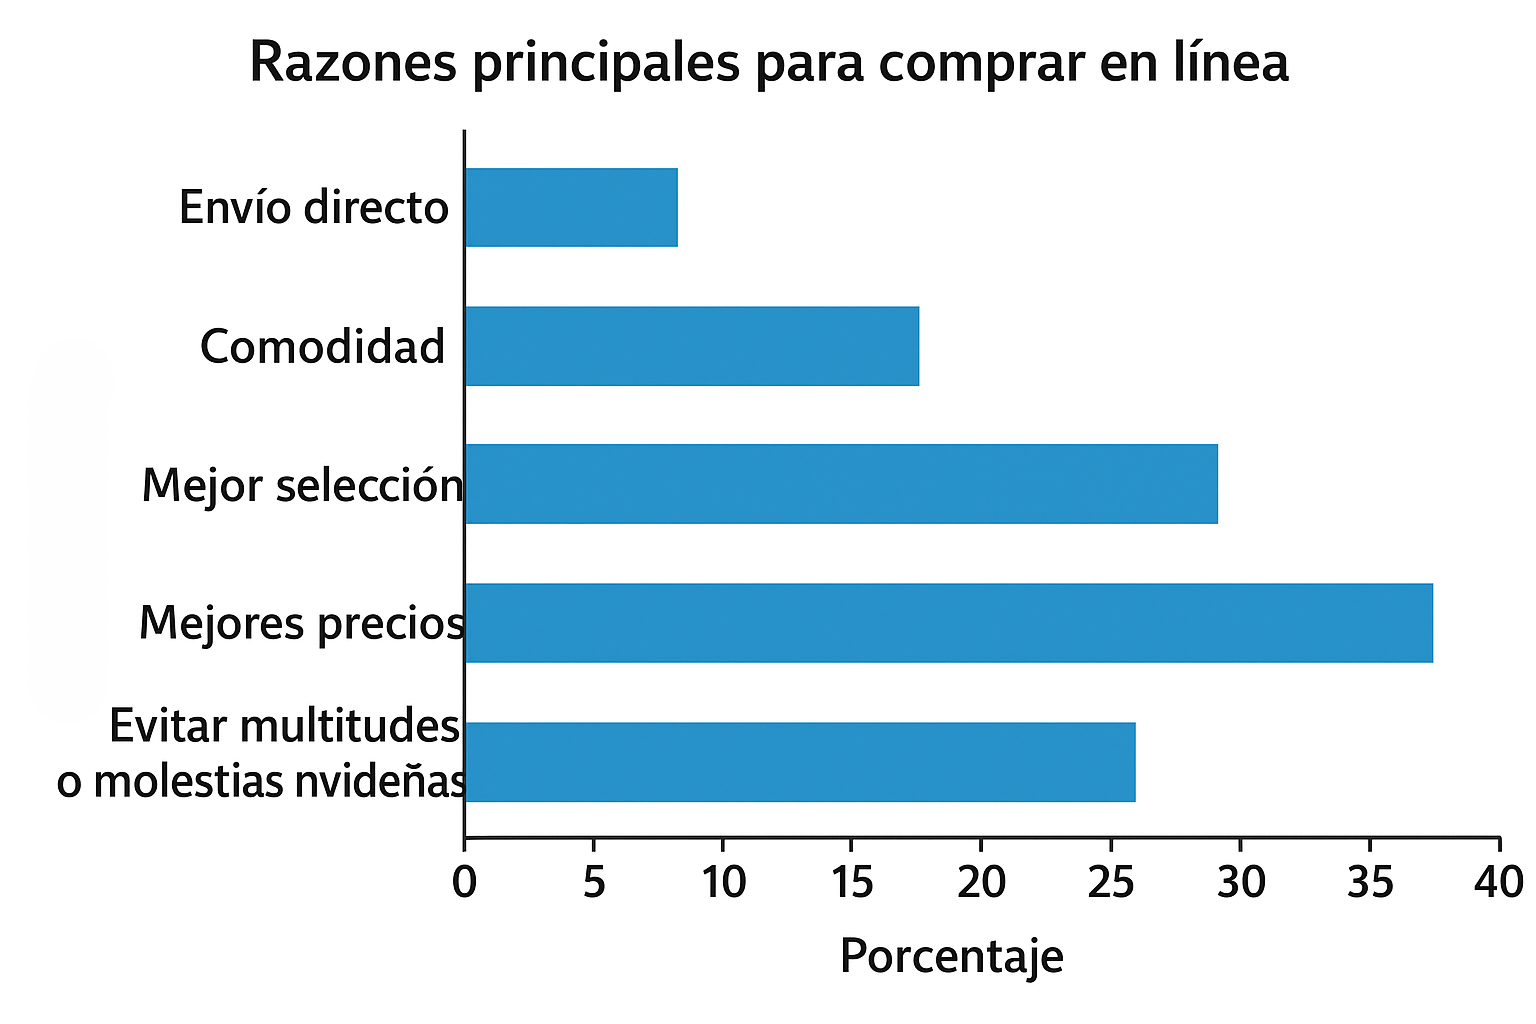
\includegraphics[keepaspectratio]{img/bar_chart.png}}

}

\caption{\label{fig-bar-chart}Ejemplo de gráfico de barras mostrando la
distribución de calificaciones}

\end{figure}%

\subsubsection{Gráfico de Torta (Pie
Chart)}\label{gruxe1fico-de-torta-pie-chart}

Los gráficos de torta representan datos categóricos como sectores de un
círculo, donde cada sector es proporcional al porcentaje que representa
esa categoría del total. La ``torta'' completa suma siempre 100\%, y
cada ``rebanada'' muestra visualmente qué proporción ocupa cada
categoría.

Su principal fortaleza es mostrar la \textbf{composición del total} - es
decir, cómo se distribuye un todo entre sus partes. Son especialmente
útiles cuando queremos enfatizar que una categoría domina sobre las
demás o cuando la pregunta clave es ``¿qué porcentaje del total
representa cada grupo?''. Por ejemplo, para mostrar la participación de
mercado de diferentes marcas o la distribución del presupuesto entre
departamentos. Este sería el gráfico de torta que muestra la misma
información del gráfico de barras anterior:

\begin{figure}

\centering{

\pandocbounded{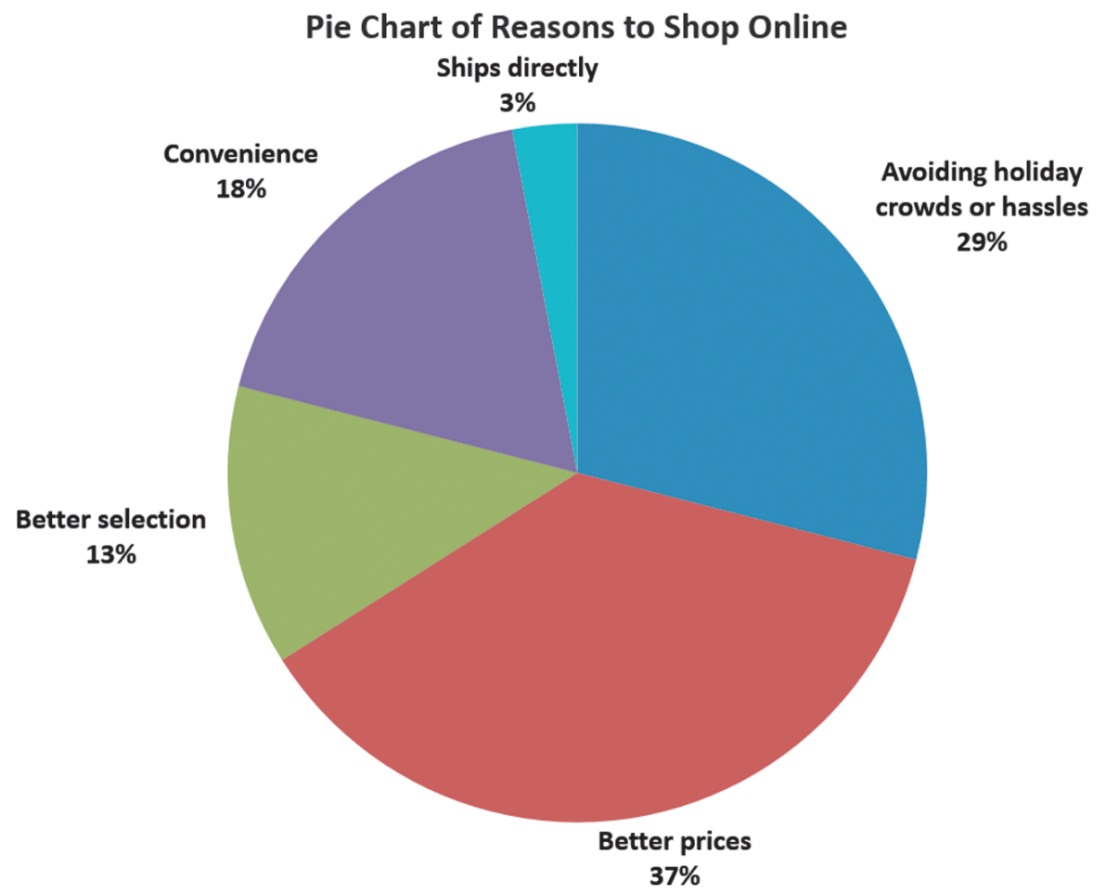
\includegraphics[keepaspectratio]{img/pie.png}}

}

\caption{\label{fig-pie-chart}Ejemplo de gráfico de torta mostrando la
distribución de calificaciones}

\end{figure}%

\begin{tcolorbox}[enhanced jigsaw, toptitle=1mm, opacitybacktitle=0.6, leftrule=.75mm, arc=.35mm, title=\textcolor{quarto-callout-warning-color}{\faExclamationTriangle}\hspace{0.5em}{Limitaciones del gráfico de torta}, colback=white, bottomrule=.15mm, colbacktitle=quarto-callout-warning-color!10!white, opacityback=0, bottomtitle=1mm, breakable, rightrule=.15mm, coltitle=black, left=2mm, titlerule=0mm, colframe=quarto-callout-warning-color-frame, toprule=.15mm]

\begin{itemize}
\tightlist
\item
  \textbf{Difícil comparación de sectores similares:} El ojo humano no
  distingue bien diferencias pequeñas entre ángulos
\item
  \textbf{Máximo recomendado:} No más de 5-7 categorías para mantener
  legibilidad
\item
  \textbf{Mejor alternativa:} Considera un gráfico de barras si
  necesitas comparar categorías con valores muy cercanos
\end{itemize}

\end{tcolorbox}

Los gráficos de torta funcionan mejor cuando hay una o dos categorías
claramente dominantes y el resto son minoritarias. Si todas las
categorías tienen tamaños similares, un gráfico de barras será más
efetorctivo para la comparación visual.

\subsubsection{Gráfico de Pareto}\label{gruxe1fico-de-pareto}

El gráfico de Pareto combina barras y una línea para identificar las
categorías más importantes según el \textbf{principio de Pareto} (regla
80-20). Las barras muestran las frecuencias ordenadas de mayor a menor,
mientras que la línea representa el porcentaje acumulado hasta llegar al
100\%.

Su objetivo principal es \textbf{priorizar} - ayuda a identificar las
pocas categorías que concentran la mayor parte del problema o fenómeno.
Por ejemplo, en control de calidad, unas pocas causas suelen generar la
mayoría de los defectos; en ventas, unos pocos productos pueden generar
la mayor parte de los ingresos.

\textbf{Elementos clave del gráfico de Pareto:}

\begin{itemize}
\tightlist
\item
  \textbf{Barras ordenadas:} De mayor a menor frecuencia (izquierda a
  derecha)
\item
  \textbf{Línea acumulada:} Muestra el porcentaje que suman las
  categorías hasta ese punto
\item
  \textbf{Principio 80-20:} Busca el punto donde pocas categorías
  explican la mayoría del fenómeno
\end{itemize}

\begin{figure}

\centering{

\pandocbounded{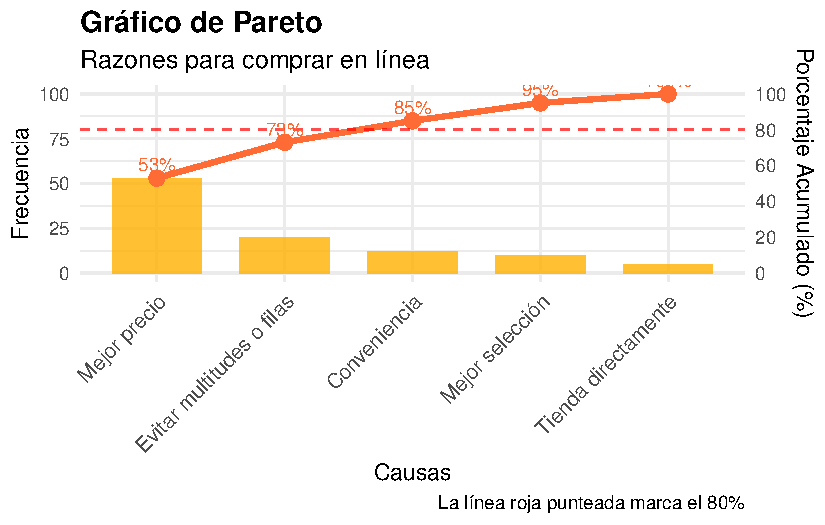
\includegraphics[keepaspectratio]{capitulo2_files/figure-pdf/fig-pareto-chart-1.pdf}}

}

\caption{\label{fig-pareto-chart}Gráfico de Pareto - Análisis de Causas
de Defectos}

\end{figure}%

\begin{tcolorbox}[enhanced jigsaw, toptitle=1mm, opacitybacktitle=0.6, leftrule=.75mm, arc=.35mm, title=\textcolor{quarto-callout-tip-color}{\faLightbulb}\hspace{0.5em}{¿Cuándo usar un gráfico de Pareto?}, colback=white, bottomrule=.15mm, colbacktitle=quarto-callout-tip-color!10!white, opacityback=0, bottomtitle=1mm, breakable, rightrule=.15mm, coltitle=black, left=2mm, titlerule=0mm, colframe=quarto-callout-tip-color-frame, toprule=.15mm]

\begin{itemize}
\tightlist
\item
  \textbf{Identificar prioridades:} ¿Qué problemas atender primero?
\item
  \textbf{Análisis de causas:} ¿Qué factores tienen mayor impacto?
\item
  \textbf{Optimización de recursos:} ¿Dónde enfocar los esfuerzos?
\item
  \textbf{Seguimiento de mejoras:} ¿Las acciones redujeron las causas
  principales?
\end{itemize}

\end{tcolorbox}

\textbf{Ejemplo práctico:} Si analizamos las quejas de un restaurante y
encontramos que ``comida fría'' y ``tiempo de espera'' representan el
75\% de todas las quejas, sabemos que resolver estos dos problemas
tendrá el mayor impacto en la satisfacción del cliente. El gráfico de
Pareto haría visible esta concentración de manera inmediata.

\subsection{Visualizando datos categóricos: Gráfico de Barras
Emparejadas}\label{visualizando-datos-categuxf3ricos-gruxe1fico-de-barras-emparejadas}

El \textbf{gráfico de barras emparejadas} (o agrupadas) se utiliza
cuando queremos comparar cómo se distribuye una variable categórica
principal dentro de los niveles de otra variable categórica. Cada grupo
del eje horizontal representa una categoría de la primera variable y,
dentro de cada grupo, las barras muestran las categorías de la segunda.

\textbf{Ejemplo:} Si analizamos las calificaciones de un restaurante
(Excelente, Buena, Regular, Mala) según la hora del día en que se dejó
la reseña (Mañana, Tarde, Noche), podemos ver rápidamente en qué horario
se concentran más las opiniones positivas.\\
Este tipo de gráfico ayuda a detectar patrones de comparación entre
grupos: diferencias claras en alturas de barras indican posibles áreas
de mejora o fortalezas.

\begin{figure}

\centering{

\pandocbounded{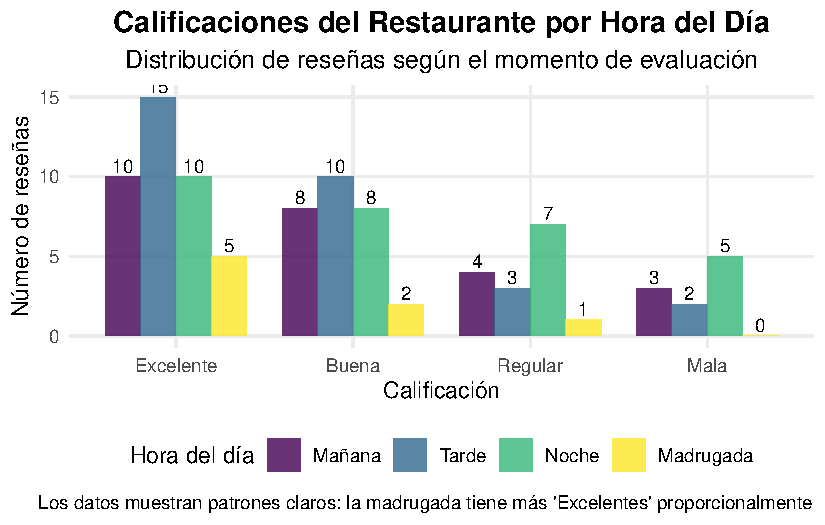
\includegraphics[keepaspectratio]{capitulo2_files/figure-pdf/fig-grouped-bars-1.pdf}}

}

\caption{\label{fig-grouped-bars}Gráfico de Barras Emparejadas -
Calificaciones por Hora del Día}

\end{figure}%

\textbf{Cuándo usarlo:}

\begin{itemize}
\tightlist
\item
  Cuando tienes \textbf{dos variables categóricas}.
\item
  Para comparar proporciones o frecuencias entre subgrupos.
\item
  Como complemento visual de una tabla de contingencia.
\end{itemize}

\textbf{Recomendaciones:}

\begin{itemize}
\tightlist
\item
  Ordena las categorías de forma lógica (por tiempo, intensidad, etc.).
\item
  Usa una leyenda clara.
\item
  Evita el exceso de colores; prioriza el contraste.
\end{itemize}

En resumen: antes de elegir cómo mostrar tus datos categóricos, conviene
pensar cuántas variables estás analizando. El siguiente esquema resume
las opciones más comunes: si trabajas con una sola variable, puedes
resumirla con una tabla y luego elegir un gráfico de barras, de torta o
de Pareto según el objetivo. Si tienes dos variables categóricas, una
tabla de contingencia es el punto de partida y suele representarse con
un gráfico de barras emparejadas para comparar grupos.

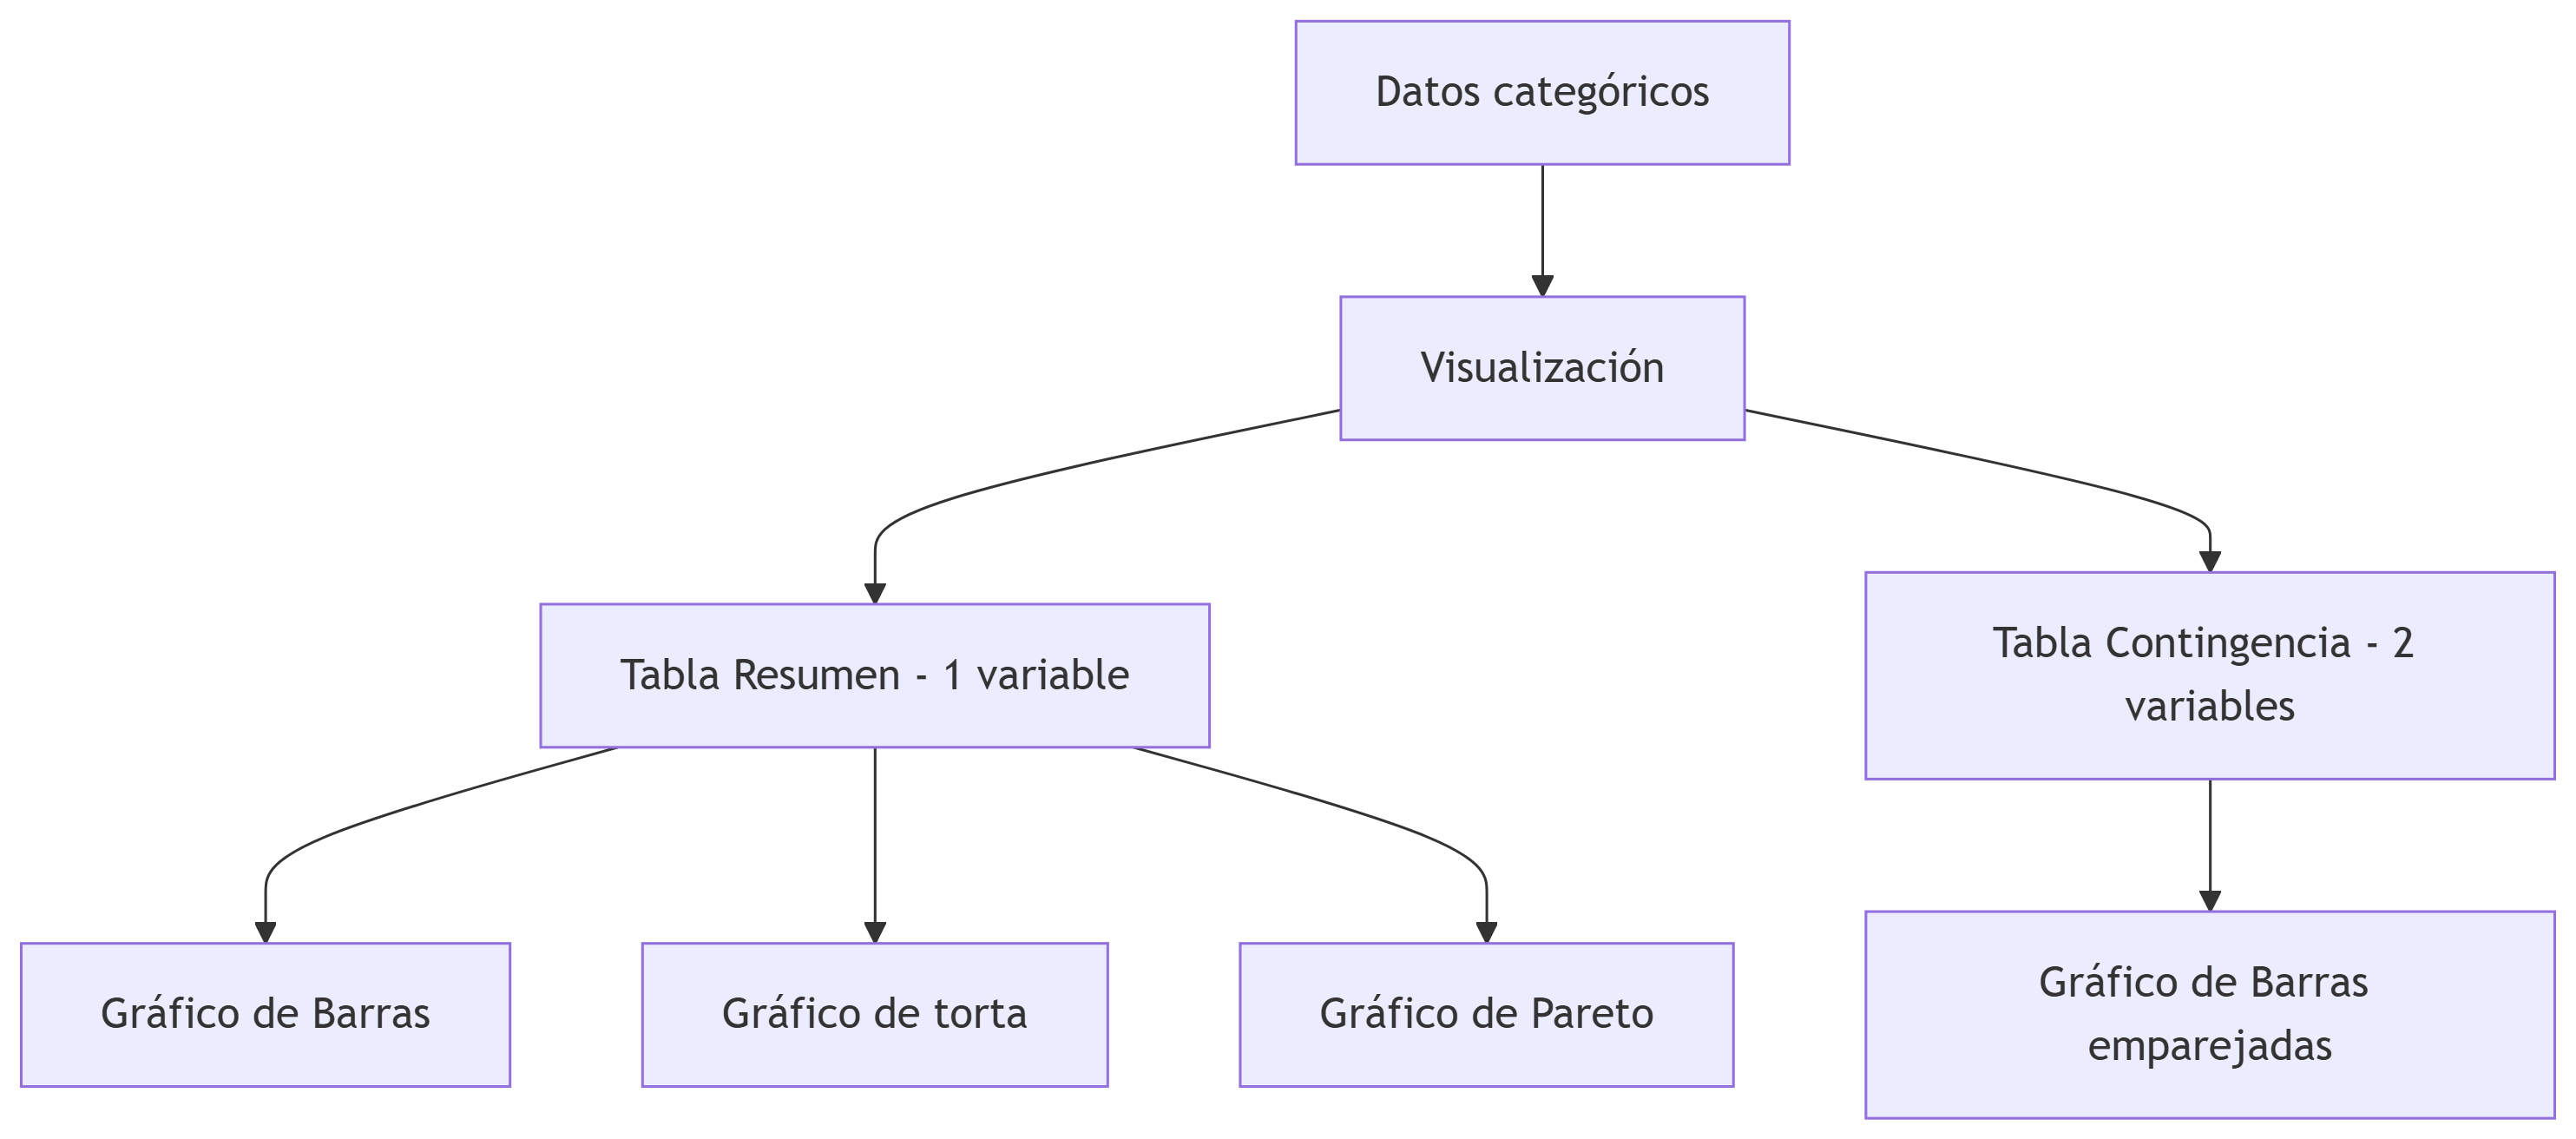
\includegraphics[width=10.13in,height=4.48in]{capitulo2_files/figure-latex/mermaid-figure-2.png}

Opciones de Visualización para Datos Categóricos

\subsection{Visualizando datos
numéricos}\label{visualizando-datos-numuxe9ricos}

\subsubsection{Distribución de
frecuencia}\label{distribuciuxf3n-de-frecuencia}

Imagina que registras el \textbf{monto gastado por cada cliente} en tu
restaurante durante un día. Tienes muchos valores sueltos y quieres
resumirlos para entender mejor los patrones.

La \textbf{distribución de frecuencia} es una tabla que agrupa esos
montos en \textbf{categorías numéricas ordenadas} (también llamadas
clases) y cuenta cuántos clientes caen en cada una.

\textbf{¿Cómo elegir las categorías?}

Primero necesitas definir \textbf{categorías adecuadas}: decidir sus
límites (fronteras) y su \textbf{ancho}.\\
El número de categorías depende del \textbf{rango} de los datos (máximo
-- mínimo). Si los gastos van desde \$5 hasta \$55, el rango es 50.\\
Cuando el rango es grande solemos usar más categorías; en la práctica,
entre \textbf{5 y 15} funciona bien.

\textbf{¿Cómo calcular el ancho?}

Si decides usar, por ejemplo, 10 categorías:

\[
\text{Ancho} = \frac{\text{Rango}}{\text{Número de categorías}} = \frac{50}{10} = 5
\]

Eso significa que tus clases podrían ser: \$5--\textless\$10,
\$10--\textless\$15, \$15--\textless\$20, \ldots{} hasta \$55. Luego
cuentas cuántos clientes gastaron en cada intervalo y obtienes una tabla
clara para analizar tendencias (por ejemplo, ``la mayoría gasta entre
\$15 y \$25'').

Esta tabla te permite pasar del desorden de datos individuales a una
visión estructurada que facilita la toma de decisiones.

\textbf{Ejemplo práctico: Distribución de gastos}

Supongamos que registramos el gasto de \textbf{100 clientes} y los
agrupamos usando intervalos de \$5:

\begin{longtable}[]{@{}
  >{\centering\arraybackslash}p{(\linewidth - 8\tabcolsep) * \real{0.2394}}
  >{\centering\arraybackslash}p{(\linewidth - 8\tabcolsep) * \real{0.1690}}
  >{\centering\arraybackslash}p{(\linewidth - 8\tabcolsep) * \real{0.1690}}
  >{\centering\arraybackslash}p{(\linewidth - 8\tabcolsep) * \real{0.2394}}
  >{\centering\arraybackslash}p{(\linewidth - 8\tabcolsep) * \real{0.1831}}@{}}
\caption{Distribución de Gastos por
Cliente}\label{tbl-distribucion-gastos}\tabularnewline
\toprule\noalign{}
\begin{minipage}[b]{\linewidth}\centering
Intervalo (USD)
\end{minipage} & \begin{minipage}[b]{\linewidth}\centering
Frecuencia
\end{minipage} & \begin{minipage}[b]{\linewidth}\centering
\% Relativo
\end{minipage} & \begin{minipage}[b]{\linewidth}\centering
Frec. Acumulada
\end{minipage} & \begin{minipage}[b]{\linewidth}\centering
\% Acumulado
\end{minipage} \\
\midrule\noalign{}
\endfirsthead
\toprule\noalign{}
\begin{minipage}[b]{\linewidth}\centering
Intervalo (USD)
\end{minipage} & \begin{minipage}[b]{\linewidth}\centering
Frecuencia
\end{minipage} & \begin{minipage}[b]{\linewidth}\centering
\% Relativo
\end{minipage} & \begin{minipage}[b]{\linewidth}\centering
Frec. Acumulada
\end{minipage} & \begin{minipage}[b]{\linewidth}\centering
\% Acumulado
\end{minipage} \\
\midrule\noalign{}
\endhead
\bottomrule\noalign{}
\endlastfoot
\$5 - \textless\$10 & 8 & 8\% & 8 & 8\% \\
\$10 - \textless\$15 & 15 & 15\% & 23 & 23\% \\
\$15 - \textless\$20 & 22 & 22\% & 45 & 45\% \\
\$20 - \textless\$25 & 25 & 25\% & 70 & 70\% \\
\$25 - \textless\$30 & 14 & 14\% & 84 & 84\% \\
\$30 - \textless\$35 & 9 & 9\% & 93 & 93\% \\
\$35 - \textless\$40 & 5 & 5\% & 98 & 98\% \\
\$40 - \textless\$45 & 2 & 2\% & 100 & 100\% \\
\textbf{Total} & \textbf{100} & \textbf{100\%} & - & - \\
\end{longtable}

\textbf{Interpretación clave:}

\begin{itemize}
\tightlist
\item
  \textbf{Concentración:} El 70\% de los clientes gastó menos de \$25
\item
  \textbf{Cola:} Solo el 7\% gastó más de \$35
\item
  \textbf{Patrón:} La mayoría de clientes (67\%) gasta entre \$10-\$30
\end{itemize}

\subsubsection{Histograma}\label{histograma}

Siguiendo con el ejemplo de los gastos en el restaurante, el
\textbf{histograma} es la versión gráfica de la tabla de distribución de
frecuencia.\\
En lugar de mostrar los números en una tabla, dibujamos una barra para
cada categoría (intervalo de gasto).

\begin{itemize}
\tightlist
\item
  El \textbf{eje horizontal} muestra los intervalos: \$5--\textless\$10,
  \$10--\textless\$15, etc.\\
\item
  El \textbf{eje vertical} muestra la frecuencia (o el porcentaje) de
  clientes en cada intervalo.\\
\item
  Las barras van \textbf{pegadas} porque los intervalos son continuos:
  representan rangos de una misma variable numérica.
\end{itemize}

\begin{figure}

\centering{

\pandocbounded{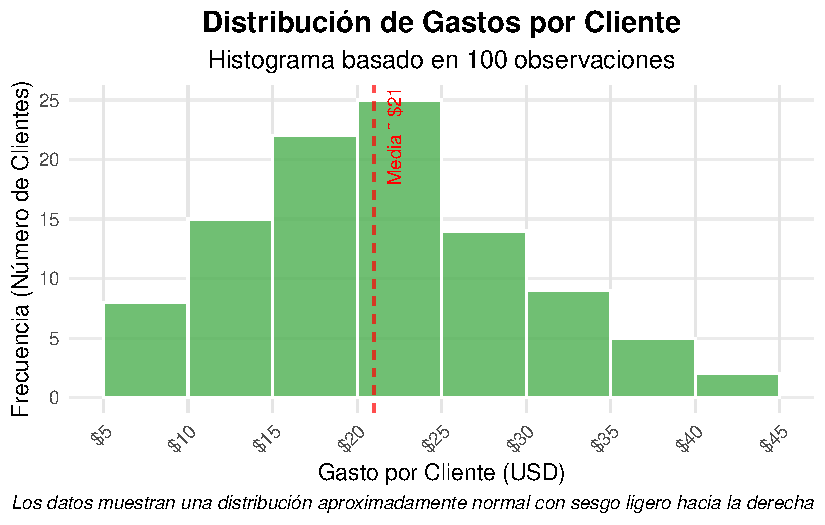
\includegraphics[keepaspectratio]{capitulo2_files/figure-pdf/fig-histograma-gastos-1.pdf}}

}

\caption{\label{fig-histograma-gastos}Histograma - Distribución de
Gastos por Cliente}

\end{figure}%

Un \textbf{histograma} es la representación gráfica de una distribución
de frecuencias para datos numéricos continuos. A diferencia del gráfico
de barras (para datos categóricos), el histograma muestra barras
adyacentes sin espacios entre ellas, lo que refleja la naturaleza
continua de los datos.

\textbf{Características clave del histograma:}

\begin{itemize}
\tightlist
\item
  \textbf{Eje X:} Intervalos de valores (clases) de la variable numérica
\item
  \textbf{Eje Y:} Frecuencia (cantidad de observaciones en cada
  intervalo)
\item
  \textbf{Barras conectadas:} Sin espacios, indicando continuidad de los
  datos
\item
  \textbf{Forma de distribución:} Permite identificar patrones como
  simetría, sesgo o multimodalidad
\end{itemize}

El histograma nos permite visualizar rápidamente:

\begin{itemize}
\tightlist
\item
  \textbf{¿Dónde se concentran los datos?} (moda o pico más alto)
\item
  \textbf{¿Cómo se distribuyen?} (simétrica, sesgada a la
  izquierda/derecha)
\item
  \textbf{¿Hay valores atípicos?} (barras aisladas en los extremos)
\end{itemize}

\begin{tcolorbox}[enhanced jigsaw, toptitle=1mm, opacitybacktitle=0.6, leftrule=.75mm, arc=.35mm, title=\textcolor{quarto-callout-note-color}{\faInfo}\hspace{0.5em}{Interpretación del histograma}, colback=white, bottomrule=.15mm, colbacktitle=quarto-callout-note-color!10!white, opacityback=0, bottomtitle=1mm, breakable, rightrule=.15mm, coltitle=black, left=2mm, titlerule=0mm, colframe=quarto-callout-note-color-frame, toprule=.15mm]

\textbf{Forma de la distribución:}

\begin{itemize}
\tightlist
\item
  \textbf{Aproximadamente normal:} La distribución tiene forma de
  campana con un pico central
\item
  \textbf{Sesgo ligero:} Hay una ``cola'' más larga hacia la derecha
  (valores altos)
\item
  \textbf{Concentración:} La mayoría de clientes gasta entre \$15-\$30
\end{itemize}

\textbf{Información práctica:}

\begin{itemize}
\tightlist
\item
  \textbf{Valor típico:} Alrededor de \$20-\$25 (pico del histograma)
\item
  \textbf{Rango común:} El 70\% de clientes gasta menos de \$25
\item
  \textbf{Valores extremos:} Muy pocos clientes gastan más de \$35
\end{itemize}

\end{tcolorbox}

\textbf{¿Cuándo usar un histograma vs.~gráfico de barras?}

\begin{longtable}[]{@{}
  >{\raggedright\arraybackslash}p{(\linewidth - 4\tabcolsep) * \real{0.2439}}
  >{\raggedright\arraybackslash}p{(\linewidth - 4\tabcolsep) * \real{0.2927}}
  >{\raggedright\arraybackslash}p{(\linewidth - 4\tabcolsep) * \real{0.4634}}@{}}
\caption{Histograma vs.~Gráfico de
Barras}\label{tbl-histograma-vs-barras}\tabularnewline
\toprule\noalign{}
\begin{minipage}[b]{\linewidth}\raggedright
Criterio
\end{minipage} & \begin{minipage}[b]{\linewidth}\raggedright
Histograma
\end{minipage} & \begin{minipage}[b]{\linewidth}\raggedright
Gráfico de Barras
\end{minipage} \\
\midrule\noalign{}
\endfirsthead
\toprule\noalign{}
\begin{minipage}[b]{\linewidth}\raggedright
Criterio
\end{minipage} & \begin{minipage}[b]{\linewidth}\raggedright
Histograma
\end{minipage} & \begin{minipage}[b]{\linewidth}\raggedright
Gráfico de Barras
\end{minipage} \\
\midrule\noalign{}
\endhead
\bottomrule\noalign{}
\endlastfoot
\textbf{Tipo de datos} & Numéricos continuos & Categóricos \\
\textbf{Separación de barras} & Sin espacios (datos continuos) & Con
espacios (categorías distintas) \\
\textbf{Objetivo principal} & Mostrar distribución de frecuencias &
Comparar categorías \\
\textbf{Ejemplo} & Edades, pesos, tiempos & Colores, marcas, géneros \\
\end{longtable}

\subsubsection{Gráfico de Dispersión}\label{gruxe1fico-de-dispersiuxf3n}

El \textbf{gráfico de dispersión} (scatter plot) es la herramienta
principal para visualizar la \textbf{relación entre dos variables
numéricas}. A diferencia del histograma que muestra una sola variable,
el gráfico de dispersión permite explorar si existe algún patrón,
tendencia o correlación entre dos mediciones diferentes.

Sigamos con el restaurante: además del \textbf{gasto de cada cliente}
(en dólares), registramos el \textbf{tiempo que permanecen} en el
establecimiento (en minutos). Queremos saber si existe alguna relación
entre estas dos variables continuas.

En el gráfico de dispersión: - Cada \textbf{punto} representa a un
cliente individual. - El \textbf{eje X} muestra el tiempo de permanencia
(en minutos). - El \textbf{eje Y} muestra el gasto total de ese cliente
(en dólares).

\textbf{Patrones que puedes identificar:}

\begin{tcolorbox}[enhanced jigsaw, toptitle=1mm, opacitybacktitle=0.6, leftrule=.75mm, arc=.35mm, title=\textcolor{quarto-callout-tip-color}{\faLightbulb}\hspace{0.5em}{Tipos de relaciones en un gráfico de dispersión}, colback=white, bottomrule=.15mm, colbacktitle=quarto-callout-tip-color!10!white, opacityback=0, bottomtitle=1mm, breakable, rightrule=.15mm, coltitle=black, left=2mm, titlerule=0mm, colframe=quarto-callout-tip-color-frame, toprule=.15mm]

\begin{itemize}
\tightlist
\item
  \textbf{Correlación positiva:} Los puntos forman una nube que asciende
  (↗). A mayor X, mayor Y
\item
  \textbf{Correlación negativa:} Los puntos forman una nube que
  desciende (↘). A mayor X, menor Y\\
\item
  \textbf{Sin correlación:} Los puntos se distribuyen aleatoriamente sin
  patrón claro
\item
  \textbf{Correlación curvilínea:} Los puntos siguen una curva (ej.
  forma de U o parábola)
\end{itemize}

\end{tcolorbox}

\begin{figure}

\centering{

\pandocbounded{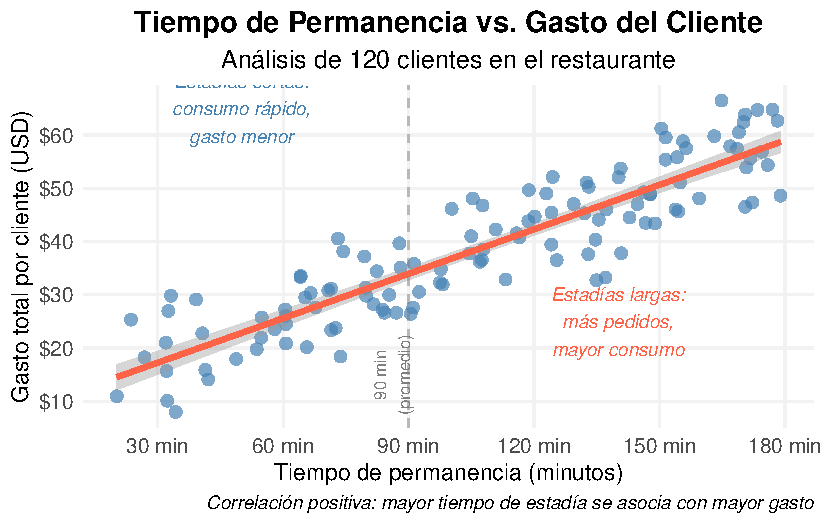
\includegraphics[keepaspectratio]{capitulo2_files/figure-pdf/fig-dispersion-tiempo-gasto-1.pdf}}

}

\caption{\label{fig-dispersion-tiempo-gasto}Gráfico de Dispersión -
Relación entre Tiempo de Permanencia y Gasto del Cliente}

\end{figure}%

\textbf{Interpretación del gráfico de dispersión:}

El ejemplo muestra una \textbf{correlación positiva} entre el tiempo de
permanencia y el gasto del cliente. Esta relación tiene sentido desde la
perspectiva del negocio:

\begin{itemize}
\tightlist
\item
  \textbf{Tendencia ascendente:} Los clientes que permanecen más tiempo
  tienden a gastar más
\item
  \textbf{Relación lógica:} Más tiempo permite más pedidos (aperitivos,
  postres, bebidas adicionales)
\item
  \textbf{Variabilidad natural:} No todos los puntos siguen la línea
  perfectamente - algunos clientes gastan mucho en poco tiempo (pedidos
  caros) y otros gastan poco aunque permanezcan mucho tiempo
\item
  \textbf{Rango de comportamientos:} Clientes con estadías cortas (20-60
  min) gastan típicamente \$8-\$30, mientras que los de estadías largas
  (120-180 min) gastan frecuentemente \$35-\$70
\end{itemize}

\textbf{Insights para el negocio:}

\begin{itemize}
\tightlist
\item
  \textbf{Estrategia de retención:} Mantener a los clientes más tiempo
  puede \textbf{incrementar las ventas}
\item
  \textbf{Ambiente acogedor:} Espacios cómodos que inviten a quedarse
  más tiempo
\item
  \textbf{Menú estratégico:} Ofrecer aperitivos, postres y bebidas para
  \textbf{extender la experiencia}
\item
  \textbf{Identificar oportunidades:} Clientes con estadías largas pero
  bajo gasto podrían necesitar más atención del mesero
\end{itemize}

\begin{tcolorbox}[enhanced jigsaw, toptitle=1mm, opacitybacktitle=0.6, leftrule=.75mm, arc=.35mm, title=\textcolor{quarto-callout-note-color}{\faInfo}\hspace{0.5em}{¿Cuándo usar un gráfico de dispersión?}, colback=white, bottomrule=.15mm, colbacktitle=quarto-callout-note-color!10!white, opacityback=0, bottomtitle=1mm, breakable, rightrule=.15mm, coltitle=black, left=2mm, titlerule=0mm, colframe=quarto-callout-note-color-frame, toprule=.15mm]

\textbf{Ideal para:}

\begin{itemize}
\tightlist
\item
  Explorar relaciones entre dos variables numéricas
\item
  Identificar correlaciones positivas, negativas o ausencia de
  correlación\\
\item
  Detectar valores atípicos (outliers)
\item
  Validar supuestos antes de análisis estadísticos más avanzados
\end{itemize}

\textbf{Limitaciones:}

\begin{itemize}
\tightlist
\item
  Solo muestra dos variables a la vez
\item
  La correlación no implica causalidad
\item
  Puede ser difícil interpretar con muchos puntos sobrepuestos
\end{itemize}

\end{tcolorbox}

\bookmarksetup{startatroot}

\chapter{Explorando tus Datos con Estadísticos
Descriptivos}\label{explorando-tus-datos-con-estaduxedsticos-descriptivos}

Imagina que eres gerente de un restaurante que acaba de lanzar un nuevo
menú y quieres evaluar la satisfacción de tus clientes a partir de las
calificaciones que te han dado. Tienes cientos de puntuaciones y
necesitas entender rápidamente cuál es la opinión general, qué tan
variadas son las experiencias y si hay patrones o valores atípicos que
merecen atención.

¿Cómo puedes resumir y comprender toda esa información de forma clara y
sencilla? Para eso utilizamos los estadísticos descriptivos,
herramientas fundamentales que nos permiten condensar grandes cantidades
de datos en medidas simples y significativas.

Estas medidas serán esenciales para tomar decisiones informadas que
mejoren tu decisiones.

\section{Estadísticos Descriptivos}\label{estaduxedsticos-descriptivos}

Los estadísticos descriptivos son herramientas clave que nos permiten
resumir y comprender mejor la información contenida en nuestros datos.
Para facilitar su estudio, los podemos clasificar en cuatro categorías
principales:

\begin{itemize}
\tightlist
\item
  \textbf{Medidas de tendencia central}: Estas nos muestran el valor
  típico o representativo en un conjunto de datos, es decir, alrededor
  de qué número se agrupan la mayoría de las observaciones.
\item
  \textbf{Medidas de variación}: Nos indican qué tan dispersos o
  concentrados están los datos respecto a esa tendencia central,
  ayudándonos a entender la consistencia o diversidad dentro de la
  información.
\item
  \textbf{Medidas de forma}: Describen la distribución general de los
  datos, revelando si están simétricos, sesgados hacia un lado o
  presentan picos o colas particulares.
\item
  \textbf{Medidas de relación}: Evalúan cómo dos variables numéricas se
  relacionan entre sí, especialmente si existe una conexión lineal que
  pueda ser útil para análisis más avanzados.
\end{itemize}

\section{Medidas de Tendencia
Central}\label{medidas-de-tendencia-central}

Cuando queremos entender las calificaciones que los clientes dan a tu
restaurante, buscamos encontrar un valor que represente lo que la
mayoría piensa. Las medidas de tendencia central nos ayudan a esto.

\subsection{Media (Promedio)}\label{media-promedio}

La media o promedio es una forma simple pero útil de resumir un conjunto
de datos. La media es el valor que obtienes al sumar todas las
calificaciones y dividirlas entre el número total de clientes.

\begin{tcolorbox}[enhanced jigsaw, colback=white, bottomrule=.15mm, opacityback=0, breakable, rightrule=.15mm, arc=.35mm, left=2mm, toprule=.15mm, colframe=quarto-callout-tip-color-frame, leftrule=.75mm]
\begin{minipage}[t]{5.5mm}
\textcolor{quarto-callout-tip-color}{\faLightbulb}
\end{minipage}%
\begin{minipage}[t]{\textwidth - 5.5mm}

Matemáticamente se escribiría así:

\[
\text{Media} = \bar{x} = \frac{x_1 + x_2 + \cdots + x_n}{n}
\]

\end{minipage}%
\end{tcolorbox}

Por ejemplo, si cinco clientes dieron las calificaciones: 4, 5, 3, 4 y
5, la media será:

\begin{tcolorbox}[enhanced jigsaw, colback=white, bottomrule=.15mm, opacityback=0, breakable, rightrule=.15mm, arc=.35mm, left=2mm, toprule=.15mm, colframe=quarto-callout-tip-color-frame, leftrule=.75mm]
\begin{minipage}[t]{5.5mm}
\textcolor{quarto-callout-tip-color}{\faLightbulb}
\end{minipage}%
\begin{minipage}[t]{\textwidth - 5.5mm}

\[
\bar{x} = \frac{4 + 5 + 3 + 4 + 5}{5} = \frac{21}{5} = 4.2
\]

\end{minipage}%
\end{tcolorbox}

Sin embargo la media, tiene limitaciones: no muestra cómo están
distribuidos los datos y puede ser engañosa si hay grandes diferencias
entre los valores. Por ejemplo:

\begin{center}
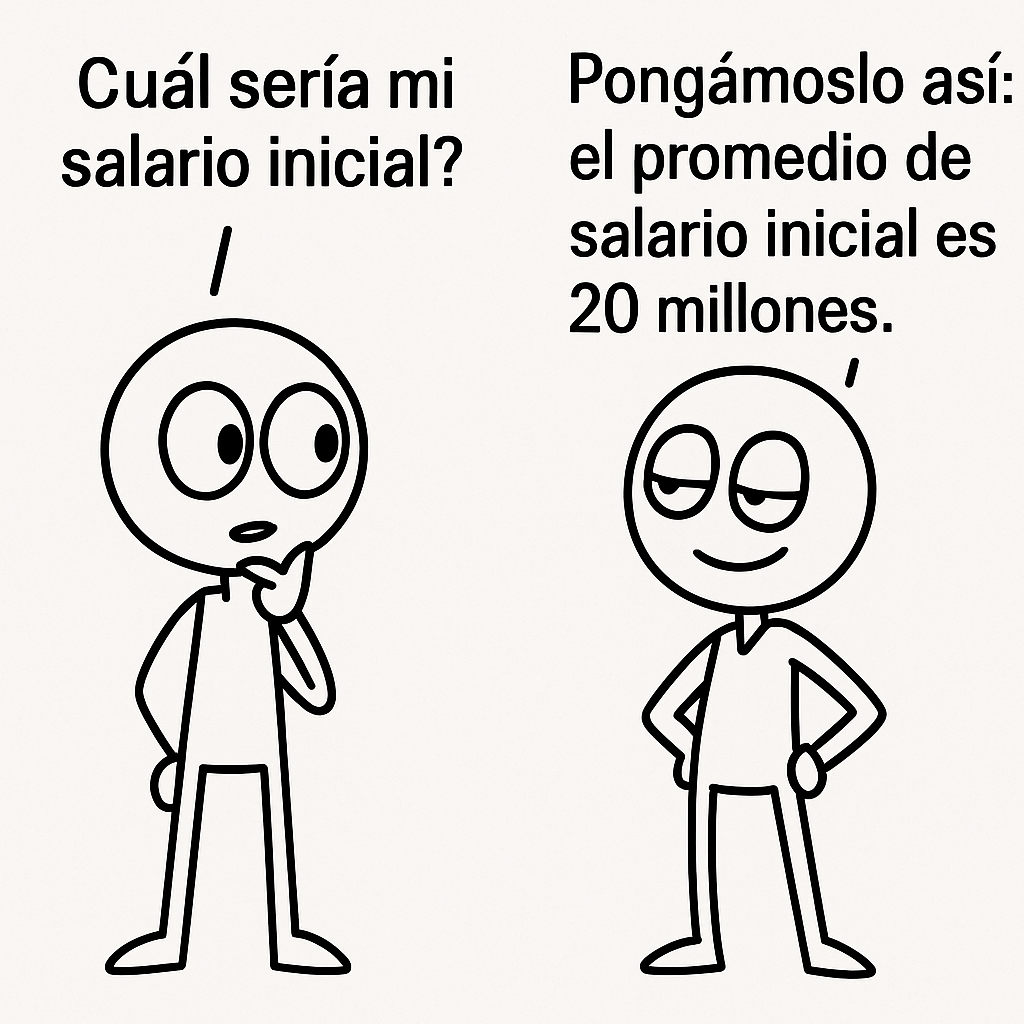
\includegraphics[width=3.64583in,height=\textheight,keepaspectratio]{img/media_1.png}
\end{center}

\begin{center}
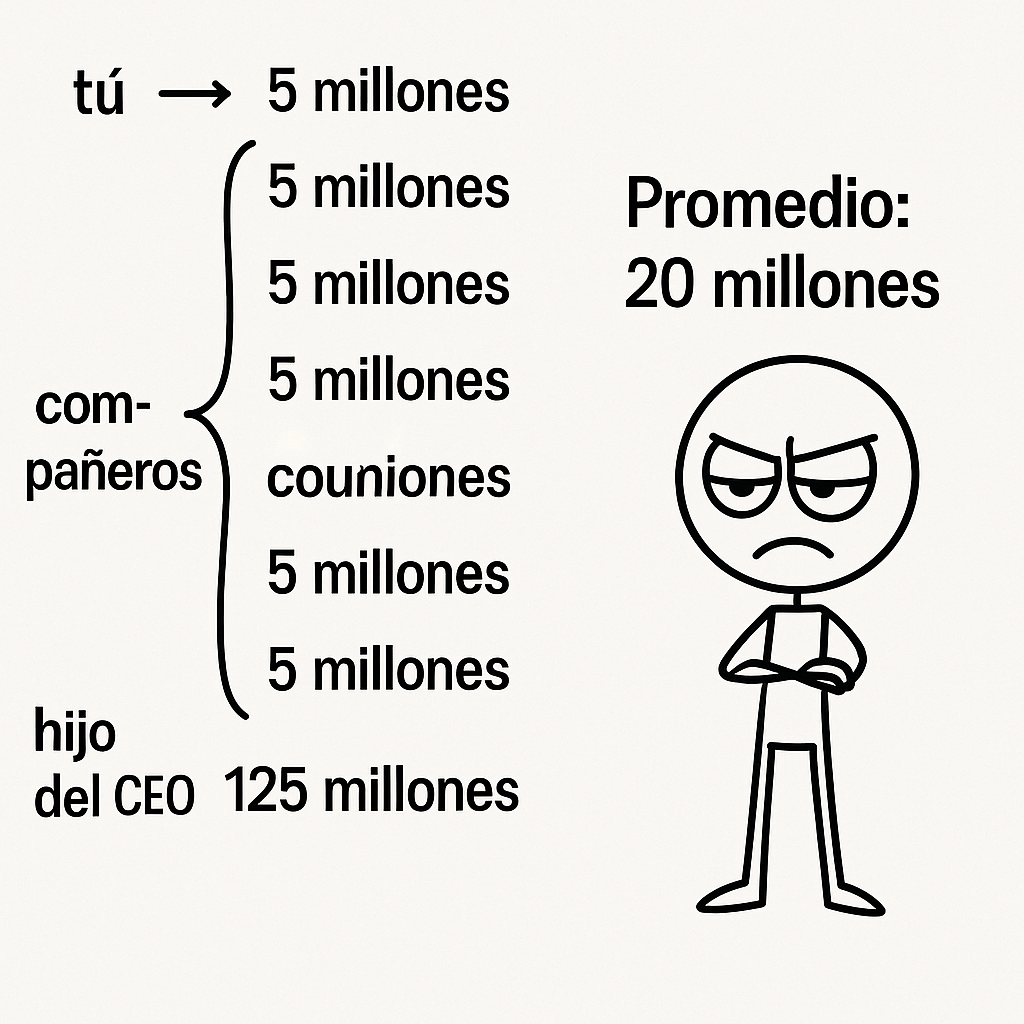
\includegraphics[width=3.64583in,height=\textheight,keepaspectratio]{img/media_2.png}
\end{center}

Aquí hay otro ejemplo donde la media es la misma en ambas situaciones
pero el contexto individual que esconde es muy diferente:

\begin{center}
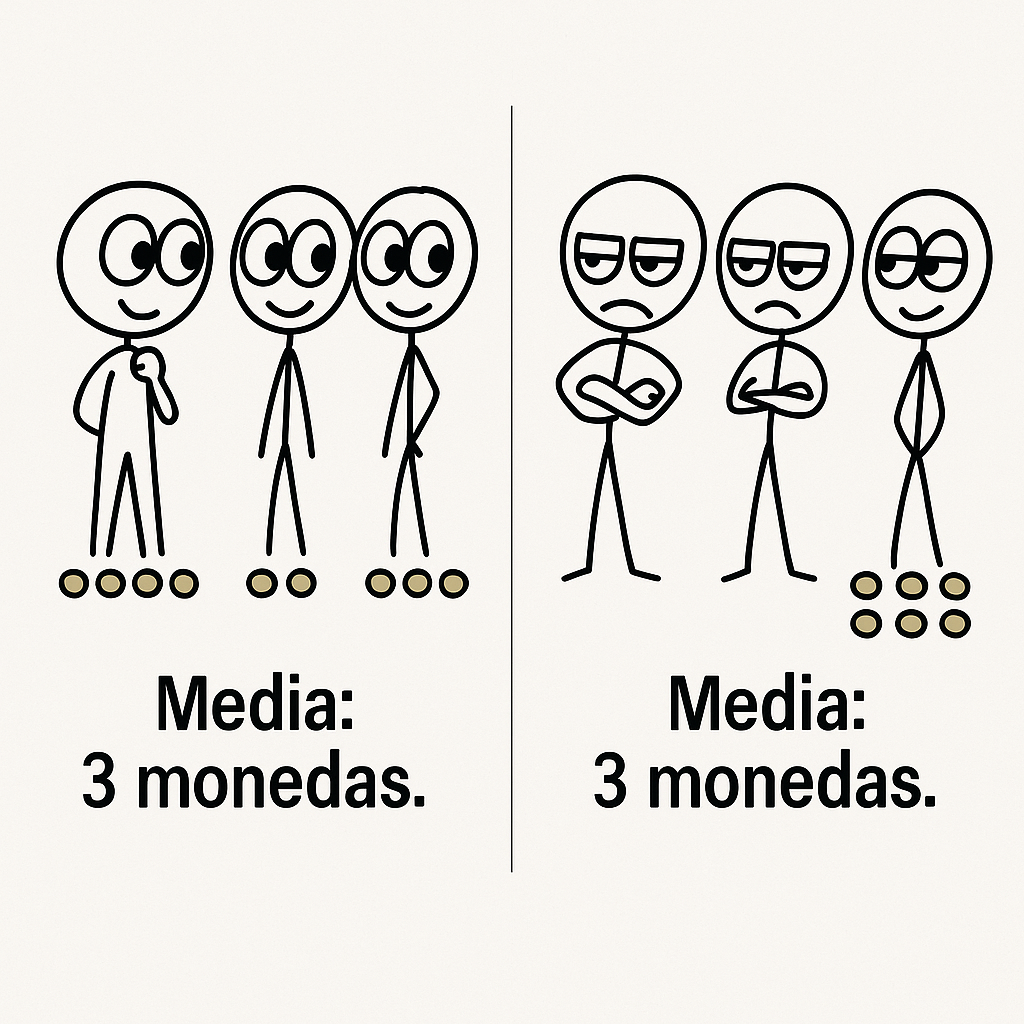
\includegraphics[width=3.64583in,height=\textheight,keepaspectratio]{img/media_3.png}
\end{center}

\subsection{Mediana}\label{mediana}

Volviendo a las calificaciones de tu restaurante, la \textbf{mediana} es
el valor que está justo en el medio cuando ordenas todas las opiniones
de menor a mayor. Esto significa que la mitad de los clientes dieron una
calificación igual o menor que la mediana, y la otra mitad dio una
calificación igual o mayor.

Por ejemplo, si tus clientes calificaron así: 3, 4, 4, 5, 5, la mediana
es 4 --- porque es el valor que divide el grupo en dos partes iguales.

\begin{tcolorbox}[enhanced jigsaw, colback=white, bottomrule=.15mm, opacityback=0, breakable, rightrule=.15mm, arc=.35mm, left=2mm, toprule=.15mm, colframe=quarto-callout-tip-color-frame, leftrule=.75mm]
\begin{minipage}[t]{5.5mm}
\textcolor{quarto-callout-tip-color}{\faLightbulb}
\end{minipage}%
\begin{minipage}[t]{\textwidth - 5.5mm}

\[
\text{Mediana} = \text{valor central en datos ordenados}
\]

\end{minipage}%
\end{tcolorbox}

Una gran ventaja de la mediana es que \textbf{no se ve afectada por
calificaciones muy bajas o muy altas} que podrían distorsionar la media.
Por ejemplo, si alguien puso un 1 o un 10, la mediana sigue mostrando el
punto medio real de la mayoría.

Sin embargo, la mediana \textbf{no nos dice qué tan dispersas están las
calificaciones a cada lado}. Por eso, para entender mejor la
variabilidad de las opiniones, necesitaremos otras medidas que veremos
más adelante.

A continuación podemos ver un ejemplo donde la mediana es usada para
entregar un mensaje erróneo:

\begin{center}
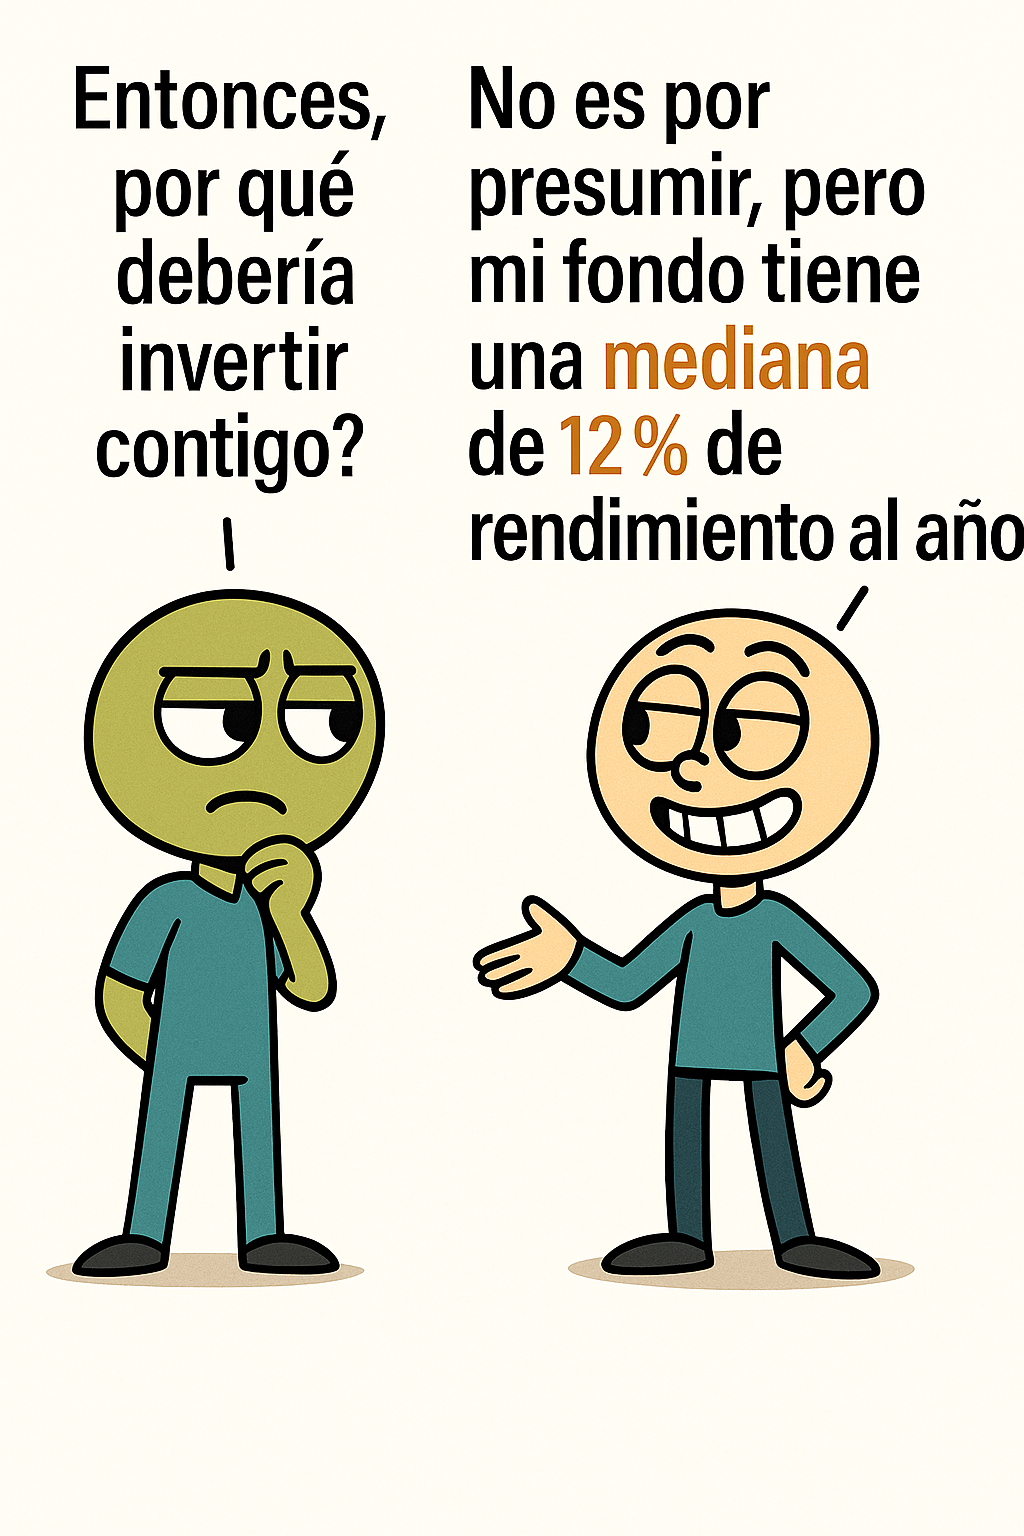
\includegraphics[width=3.64583in,height=\textheight,keepaspectratio]{img/mediana_1.png}
\end{center}

Pero, los rendimientos anuales del fondo:

\begin{center}
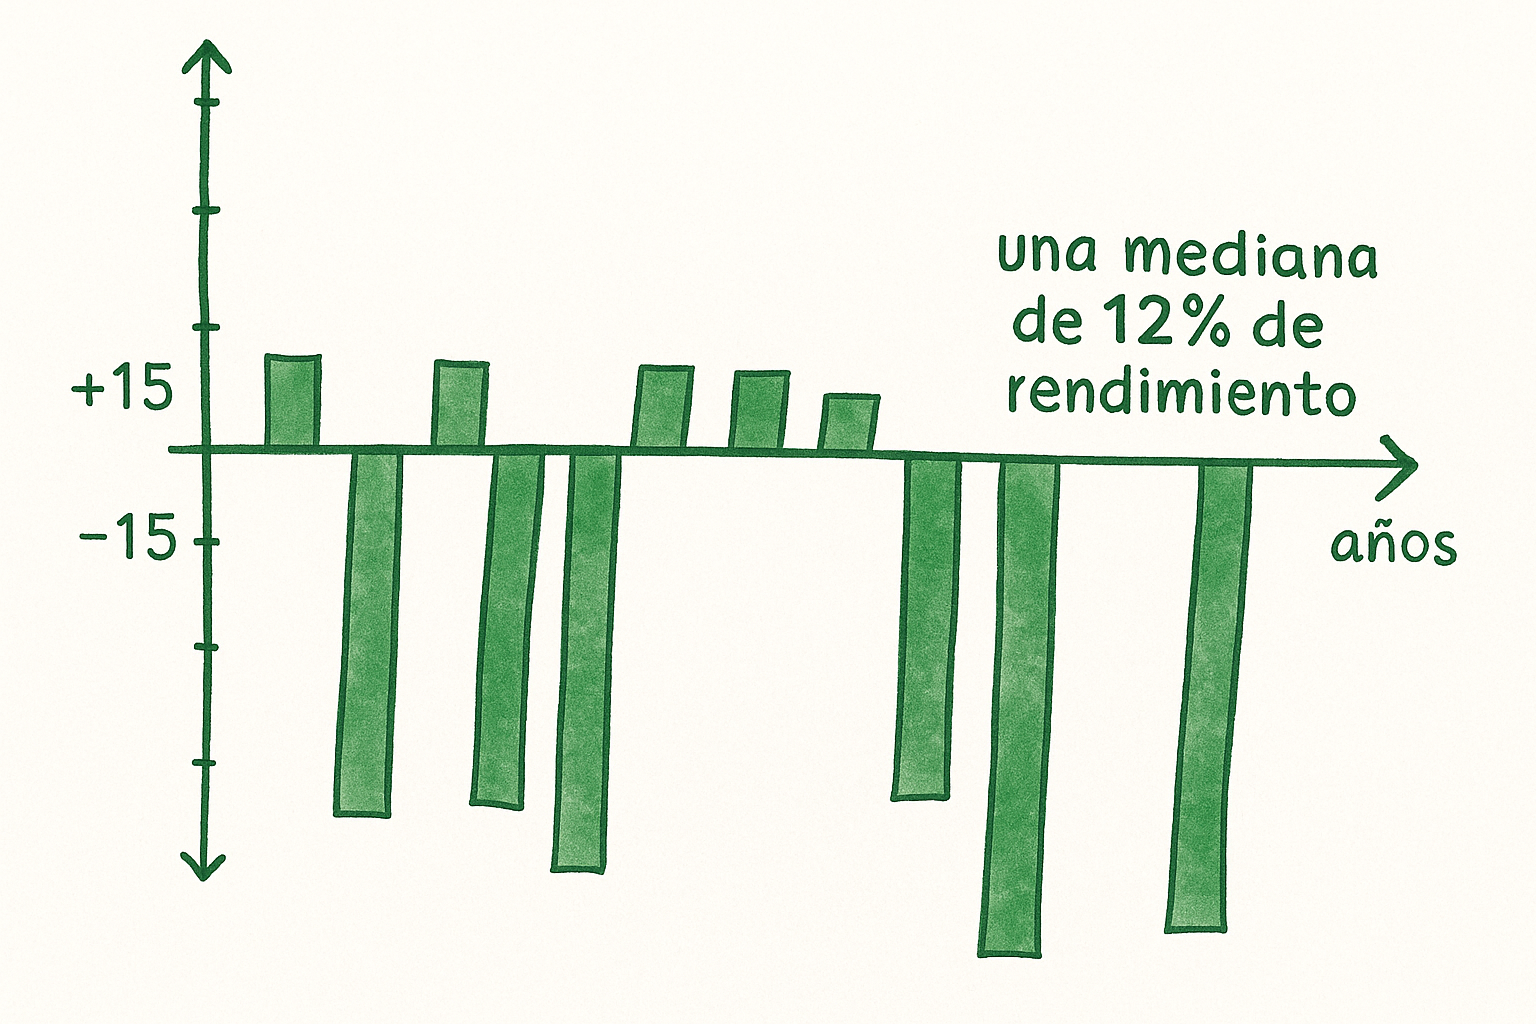
\includegraphics[width=3.64583in,height=\textheight,keepaspectratio]{img/mediana_2.png}
\end{center}

Miremos otro ejemplo donde la mediana similar no implica datos
similares. Siempre hay tener una combinación de datos para tomar
decisiones correctas

\begin{center}
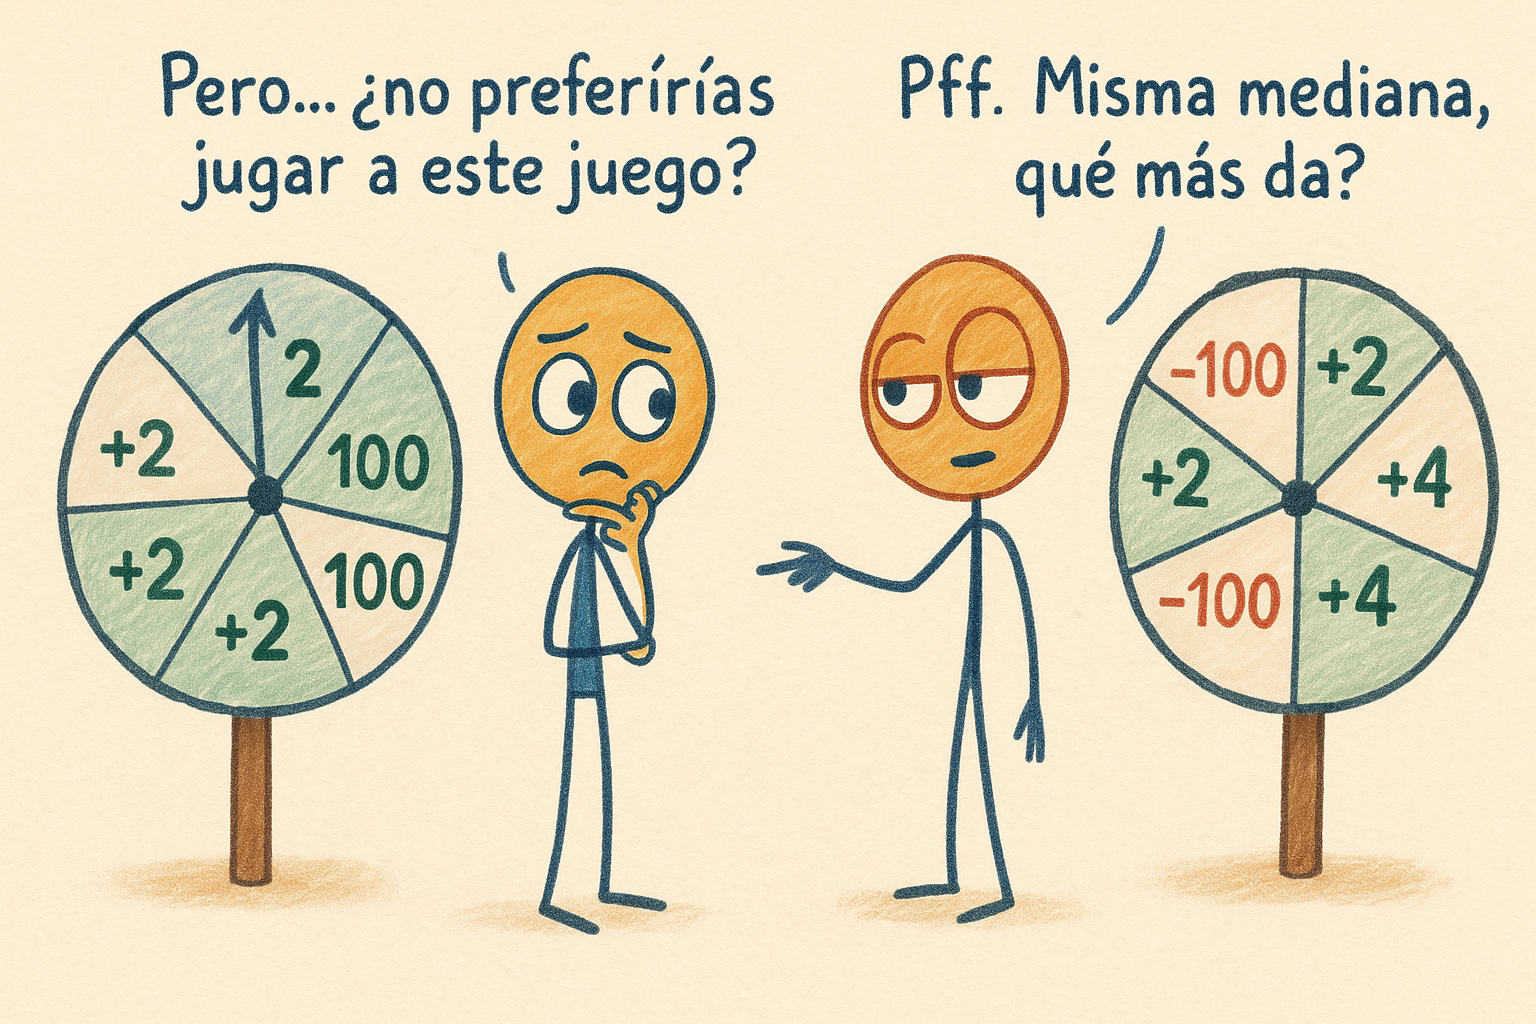
\includegraphics[width=3.64583in,height=\textheight,keepaspectratio]{img/mediana_3.png}
\end{center}

\subsection{Moda}\label{moda}

La \textbf{moda} es la calificación que más se repite entre tus
clientes. Es como la opinión más común o popular sobre tu restaurante.

Por ejemplo, si las calificaciones de tus clientes fueron: 3, 4, 4, 5,
5, tanto 4 como 5 se repiten dos veces, por lo que hay dos modas: 4 y 5.

Si no hay repeticiones exactas, se pueden agrupar en categorías y tomar
como moda la más común. Es útil especialmente con datos no numéricos,
como colores o preferencias políticas, donde no tiene sentido calcular
promedios.

\begin{tcolorbox}[enhanced jigsaw, colback=white, bottomrule=.15mm, opacityback=0, breakable, rightrule=.15mm, arc=.35mm, left=2mm, toprule=.15mm, colframe=quarto-callout-tip-color-frame, leftrule=.75mm]
\begin{minipage}[t]{5.5mm}
\textcolor{quarto-callout-tip-color}{\faLightbulb}
\end{minipage}%
\begin{minipage}[t]{\textwidth - 5.5mm}

\[
\text{Moda} = \text{valor que aparece con mayor frecuencia}
\]

\end{minipage}%
\end{tcolorbox}

Su limitación: no considera la totalidad ni la distribución de los
datos, y lo más común no siempre es lo más representativo. Miremos este
ejemplo:

\begin{center}
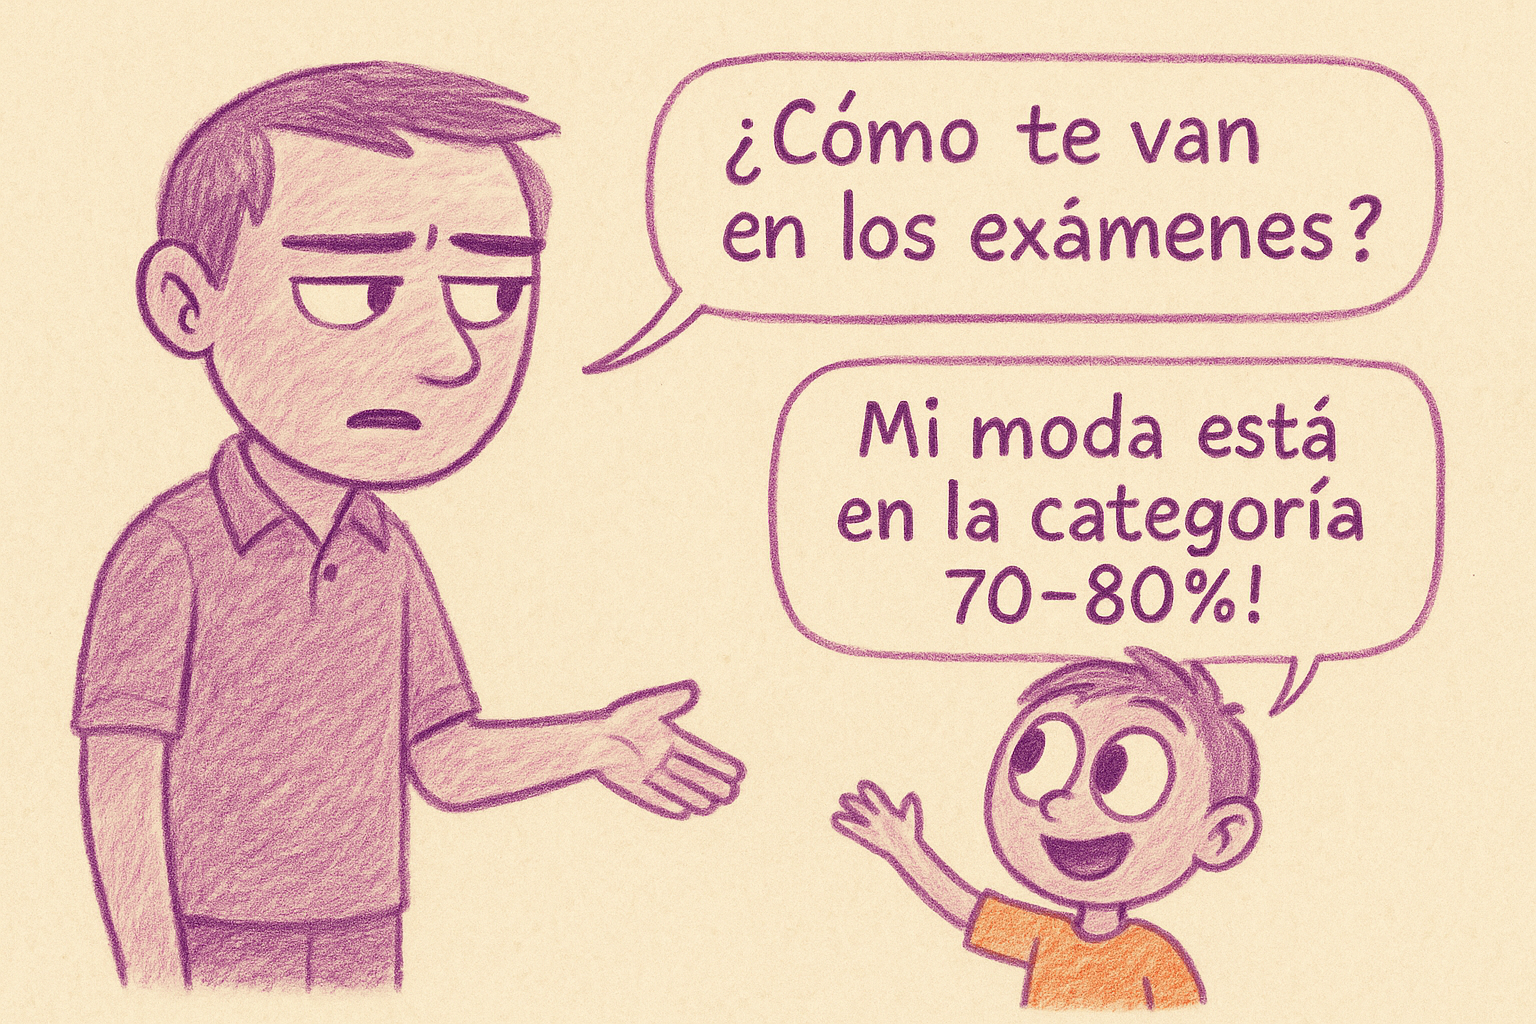
\includegraphics[width=3.64583in,height=\textheight,keepaspectratio]{img/moda_1.png}
\end{center}

\begin{center}
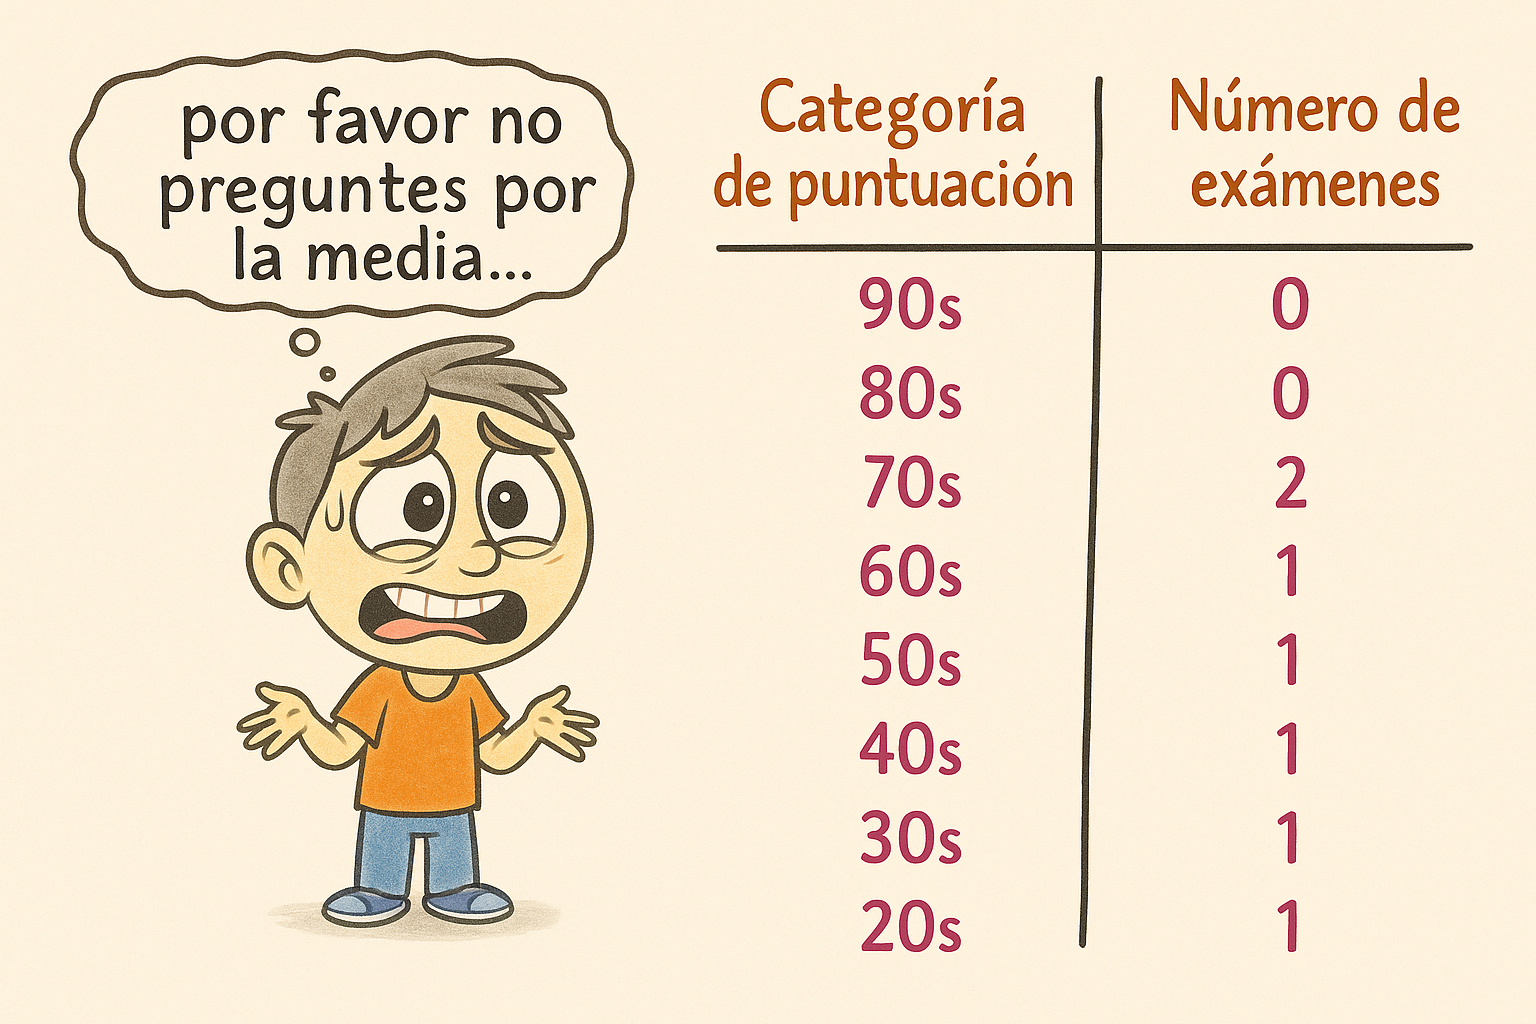
\includegraphics[width=3.64583in,height=\textheight,keepaspectratio]{img/moda_2.png}
\end{center}

\section{Medidas de Variación}\label{medidas-de-variaciuxf3n}

Las medidas de variación nos ayudan a entender qué tan diferentes o
dispersos están los datos entre sí. Es decir, nos dicen si las opiniones
o valores están muy juntos o muy separados.

\subsection{Rango}\label{rango}

Las medidas de variación nos ayudan a entender qué tan diferentes o
dispersos están los datos entre sí. Es decir, nos dicen si las opiniones
o valores están muy juntos o muy separados.

Por ejemplo, si las calificaciones en tu restaurante van desde 2 hasta
5, el rango sería:

\begin{tcolorbox}[enhanced jigsaw, colback=white, bottomrule=.15mm, opacityback=0, breakable, rightrule=.15mm, arc=.35mm, left=2mm, toprule=.15mm, colframe=quarto-callout-tip-color-frame, leftrule=.75mm]
\begin{minipage}[t]{5.5mm}
\textcolor{quarto-callout-tip-color}{\faLightbulb}
\end{minipage}%
\begin{minipage}[t]{\textwidth - 5.5mm}

\[
\text{Rango} = 5 - 2 = 3
\]

\end{minipage}%
\end{tcolorbox}

Esto nos dice que las opiniones varían en un rango de 3 puntos, desde
una calificación baja hasta una alta.

Su principal ventaja es su simplicidad, da una idea rápida del ``ancho''
del conjunto de datos.

Pero su debilidad es igual de clara, solo considera los valores
extremos, ignorando por completo todos los datos intermedios.

Miremos un ejemplo de un rango que da una impresión incorrecta:

\begin{center}
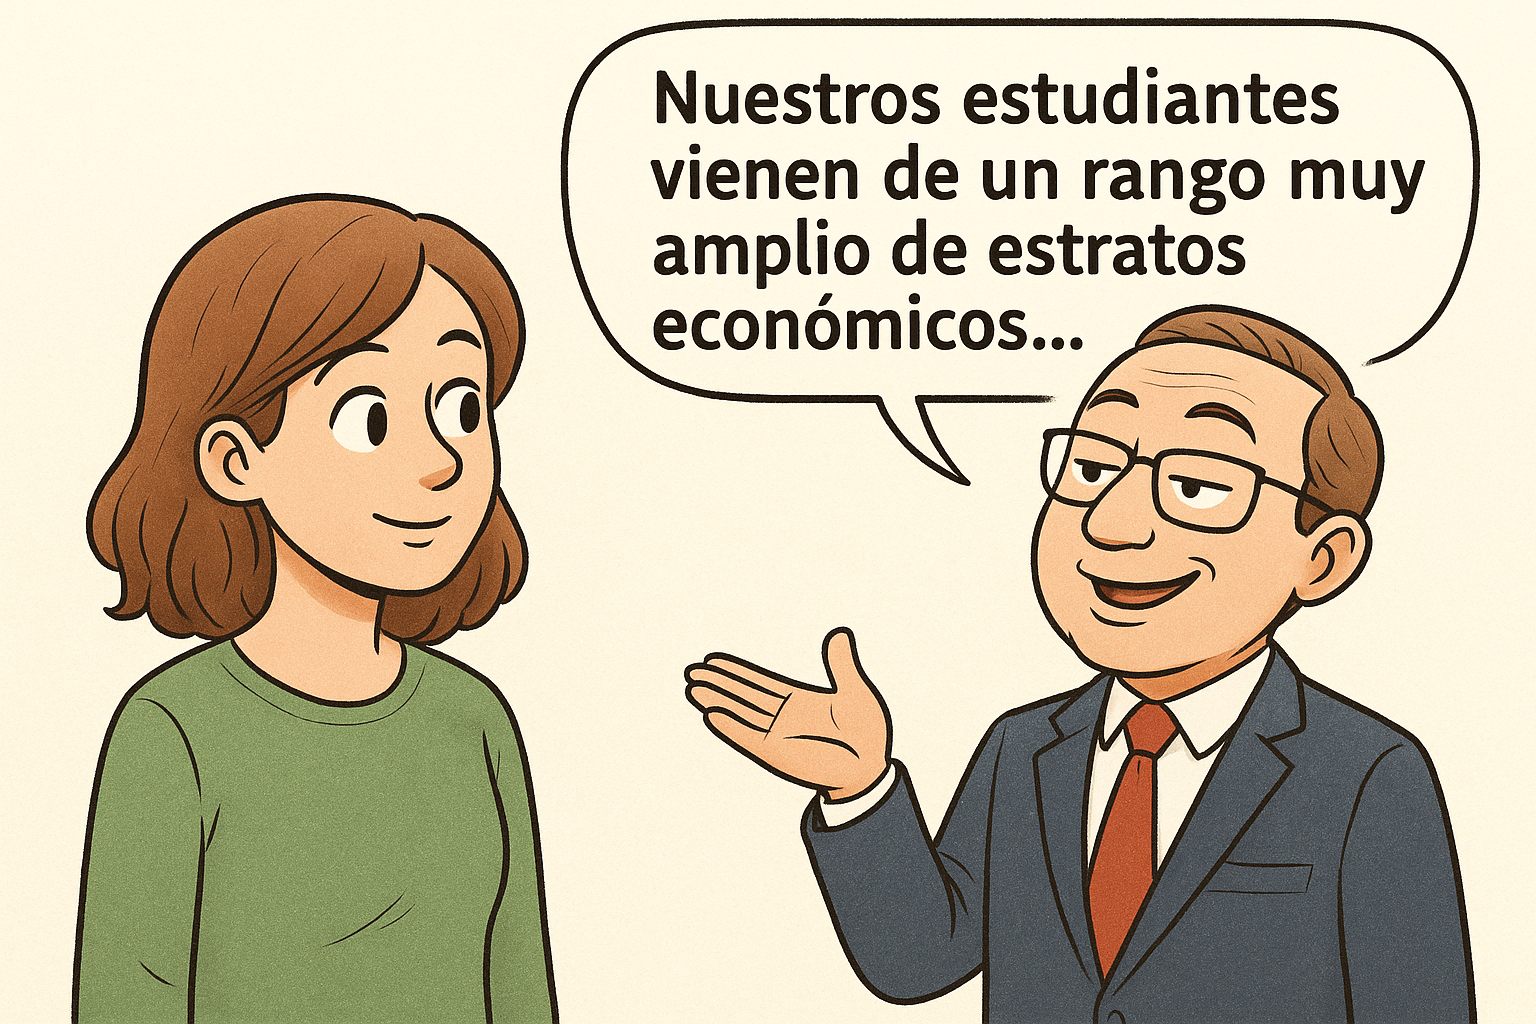
\includegraphics[width=3.64583in,height=\textheight,keepaspectratio]{img/rango_1.png}
\end{center}

\begin{center}
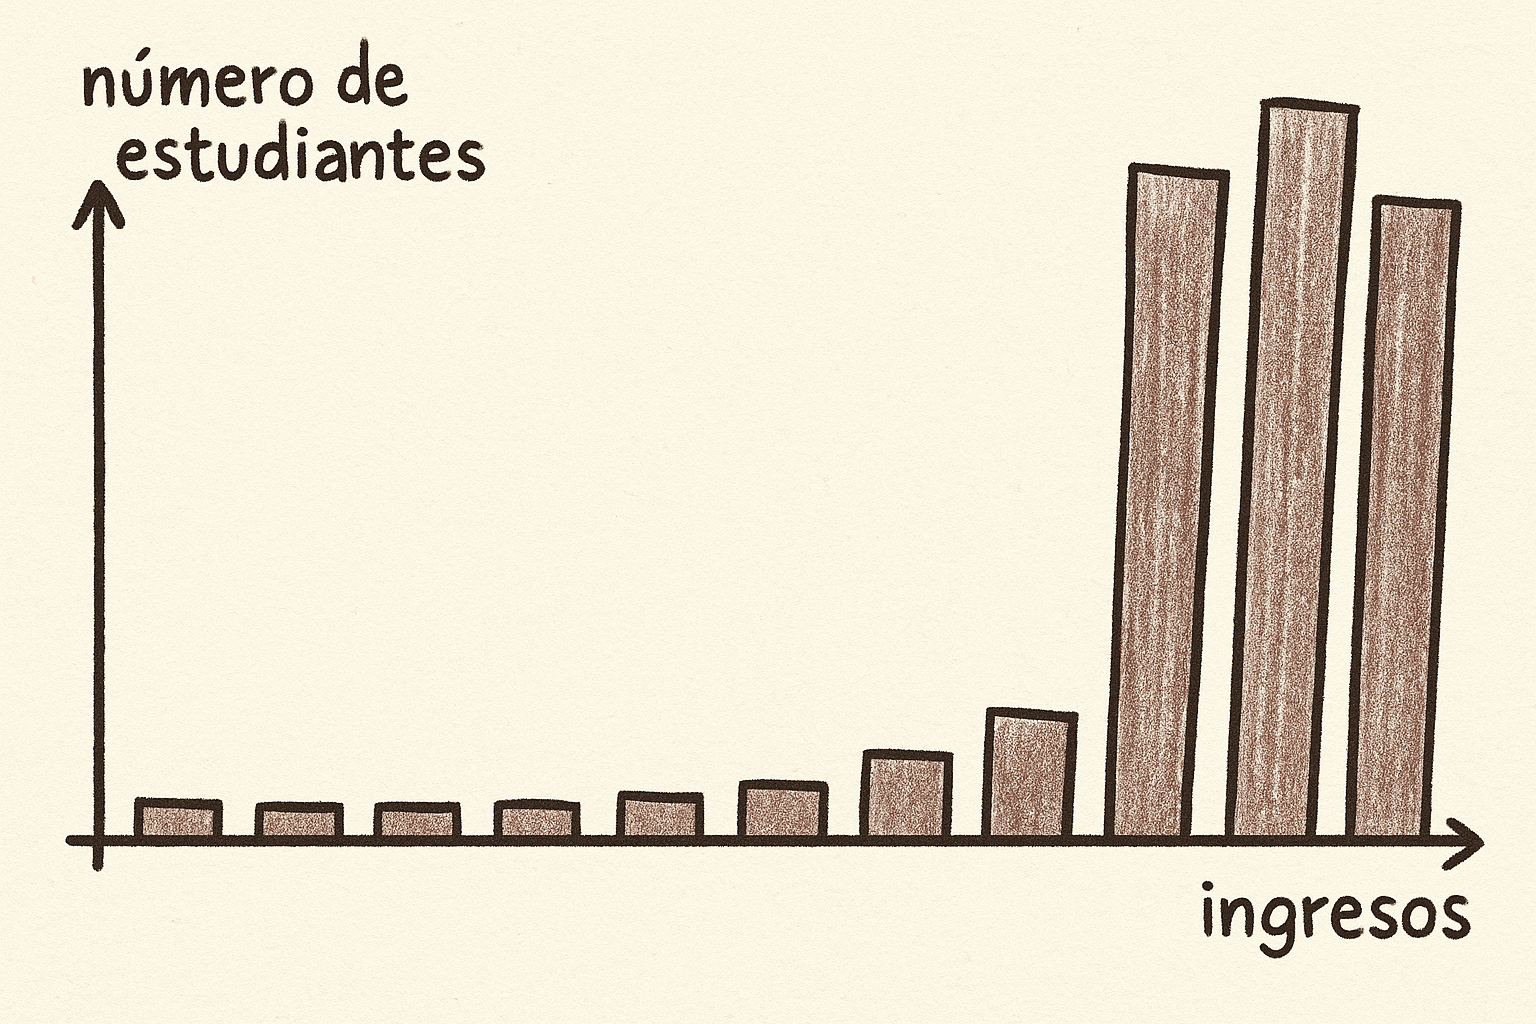
\includegraphics[width=3.64583in,height=\textheight,keepaspectratio]{img/rango_2.png}
\end{center}

\subsection{Varianza y Desviación
Estándar}\label{varianza-y-desviaciuxf3n-estuxe1ndar}

La varianza y la desviación estándar son herramientas que nos ayudan a
entender qué tan dispersos están los datos con respecto a su media.

Imagina que tienes varios números y quieres saber si están todos cerca
del promedio o si están muy separados entre sí.

Para entender qué tan dispersas están las calificaciones de tus clientes
respecto al promedio, usamos dos medidas fundamentales: la
\textbf{varianza} y la \textbf{desviación estándar}:

\begin{itemize}
\tightlist
\item
  Una desviación estándar baja significa que los datos están cerca del
  promedio.
\item
  Una alta desviación estándar indica mucha dispersión.
\end{itemize}

\begin{tcolorbox}[enhanced jigsaw, colback=white, bottomrule=.15mm, opacityback=0, breakable, rightrule=.15mm, arc=.35mm, left=2mm, toprule=.15mm, colframe=quarto-callout-tip-color-frame, leftrule=.75mm]
\begin{minipage}[t]{5.5mm}
\textcolor{quarto-callout-tip-color}{\faLightbulb}
\end{minipage}%
\begin{minipage}[t]{\textwidth - 5.5mm}

Si quisieras ``cocinar'' la varianza en tu propia cocina, la receta
sería así:

\begin{enumerate}
\def\labelenumi{\arabic{enumi}.}
\tightlist
\item
  \textbf{Encuentra la media} de todas las calificaciones.\\
\item
  \textbf{Calcula qué tan lejos está cada calificación de esa media} (la
  diferencia entre cada calificación y la media).\\
\item
  \textbf{Eleva al cuadrado cada una de esas diferencias} para evitar
  que se cancelen y para dar más peso a las diferencias grandes.\\
\item
  \textbf{Suma todas esas diferencias al cuadrado y calcula el promedio}
  dividiendo entre el número de calificaciones menos uno.
\end{enumerate}

\end{minipage}%
\end{tcolorbox}

Matemáticamente, si tienes ( n ) calificaciones ( x\_1, x\_2, \ldots,
x\_n ) y la media ( \bar\{x\} ), la varianza se calcula así:

\begin{tcolorbox}[enhanced jigsaw, colback=white, bottomrule=.15mm, opacityback=0, breakable, rightrule=.15mm, arc=.35mm, left=2mm, toprule=.15mm, colframe=quarto-callout-tip-color-frame, leftrule=.75mm]
\begin{minipage}[t]{5.5mm}
\textcolor{quarto-callout-tip-color}{\faLightbulb}
\end{minipage}%
\begin{minipage}[t]{\textwidth - 5.5mm}

\[
\text{Varianza} = s^2 = \frac{1}{n-1} \sum_{i=1}^n (x_i - \bar{x})^2
\]

\end{minipage}%
\end{tcolorbox}

Pero como la varianza está al cuadrado, no es fácil interpretarla
directamente, pues sus unidades no son las mismas que las de las
calificaciones. Por eso usamos la \textbf{desviación estándar}, que es
la raíz cuadrada de la varianza y nos da una medida en las mismas
unidades originales.

\begin{tcolorbox}[enhanced jigsaw, colback=white, bottomrule=.15mm, opacityback=0, breakable, rightrule=.15mm, arc=.35mm, left=2mm, toprule=.15mm, colframe=quarto-callout-tip-color-frame, leftrule=.75mm]
\begin{minipage}[t]{5.5mm}
\textcolor{quarto-callout-tip-color}{\faLightbulb}
\end{minipage}%
\begin{minipage}[t]{\textwidth - 5.5mm}

\[
\text{Desviación Estándar} = s = \sqrt{s^2}
\]

\end{minipage}%
\end{tcolorbox}

Por ejemplo, si las calificaciones fueron: 4, 5, 3, 4 y 5, la media es:

\begin{tcolorbox}[enhanced jigsaw, colback=white, bottomrule=.15mm, opacityback=0, breakable, rightrule=.15mm, arc=.35mm, left=2mm, toprule=.15mm, colframe=quarto-callout-tip-color-frame, leftrule=.75mm]
\begin{minipage}[t]{5.5mm}
\textcolor{quarto-callout-tip-color}{\faLightbulb}
\end{minipage}%
\begin{minipage}[t]{\textwidth - 5.5mm}

\[
\bar{x} = \frac{4 + 5 + 3 + 4 + 5}{5} = 4.2
\]

\end{minipage}%
\end{tcolorbox}

Luego, calculamos la varianza:

\begin{tcolorbox}[enhanced jigsaw, colback=white, bottomrule=.15mm, opacityback=0, breakable, rightrule=.15mm, arc=.35mm, left=2mm, toprule=.15mm, colframe=quarto-callout-tip-color-frame, leftrule=.75mm]
\begin{minipage}[t]{5.5mm}
\textcolor{quarto-callout-tip-color}{\faLightbulb}
\end{minipage}%
\begin{minipage}[t]{\textwidth - 5.5mm}

\[
s^2 = \frac{(4 - 4.2)^2 + (5 - 4.2)^2 + (3 - 4.2)^2 + (4 - 4.2)^2 + (5 - 4.2)^2}{4} = 0.7
\]

\end{minipage}%
\end{tcolorbox}

Y finalmente, la desviación estándar es:

\begin{tcolorbox}[enhanced jigsaw, colback=white, bottomrule=.15mm, opacityback=0, breakable, rightrule=.15mm, arc=.35mm, left=2mm, toprule=.15mm, colframe=quarto-callout-tip-color-frame, leftrule=.75mm]
\begin{minipage}[t]{5.5mm}
\textcolor{quarto-callout-tip-color}{\faLightbulb}
\end{minipage}%
\begin{minipage}[t]{\textwidth - 5.5mm}

\[
s = \sqrt{0.7} \approx 0.84
\]

\end{minipage}%
\end{tcolorbox}

Esto significa que, en promedio, las calificaciones se alejan de la
media en aproximadamente 0.84 puntos.

A diferencia del rango, que solo considera los valores más extremos, la
varianza y la desviación estándar toman en cuenta todos los datos. Por
eso ofrecen una visión más completa de la dispersión. Sin embargo,
también tienen una desventaja: si hay un solo valor muy alejado (un
valor extremo), puede aumentar mucho la varianza, aunque la mayoría de
los datos estén cerca de la media. Mira el ejemplo a continuación, para
entenderlo mejor:

\begin{center}
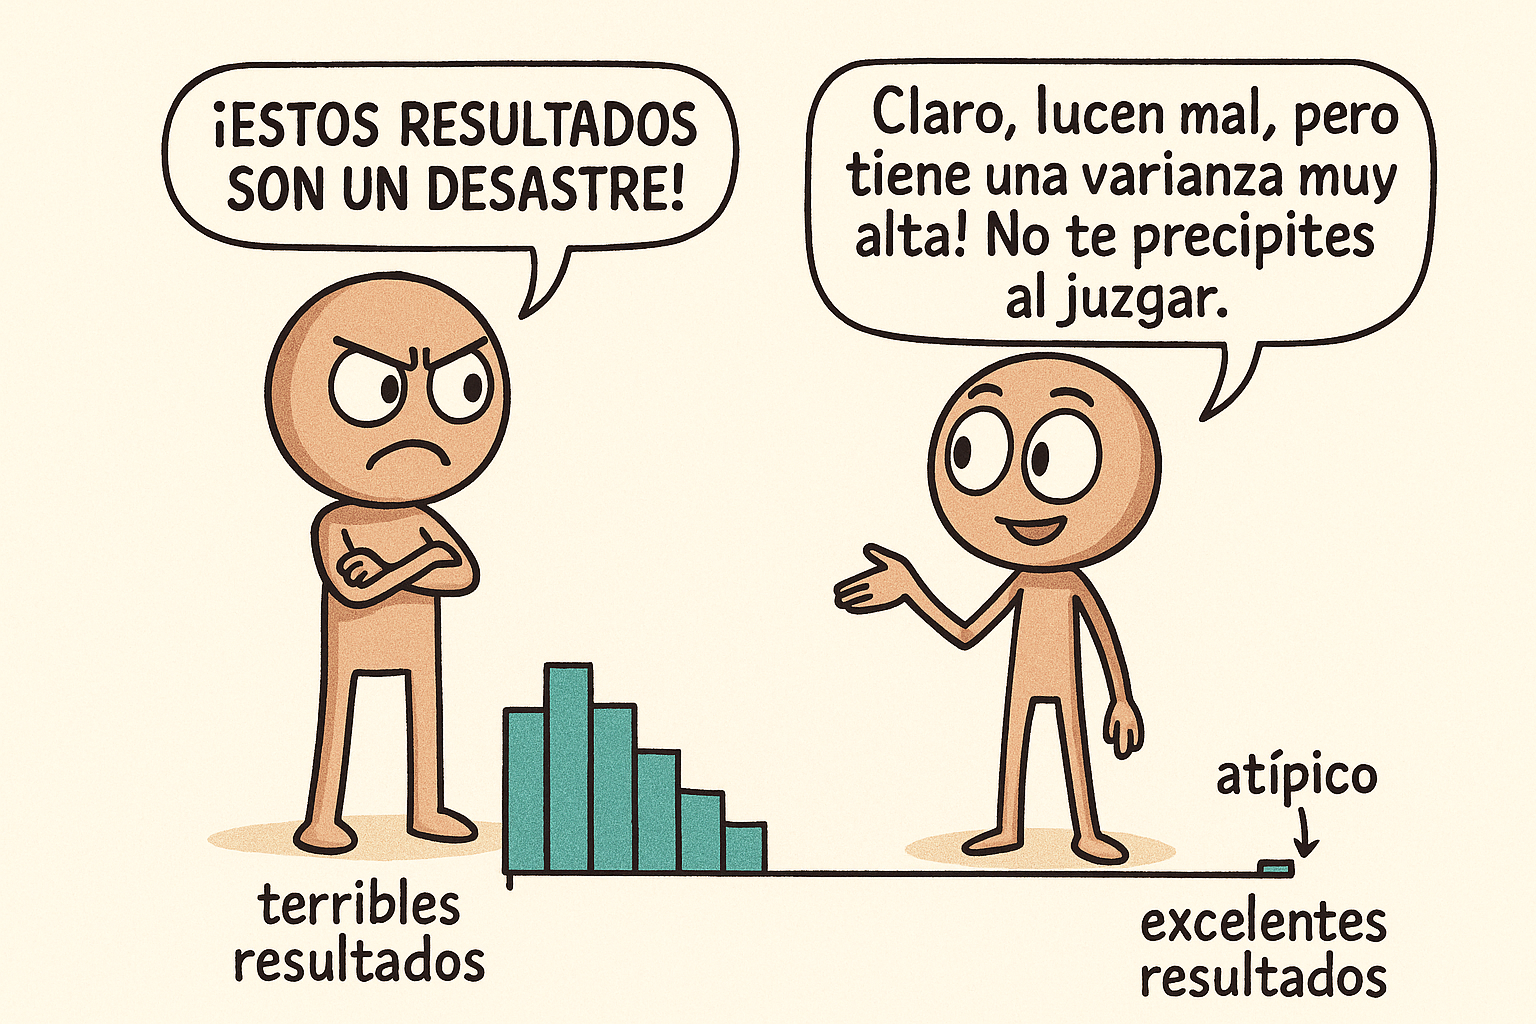
\includegraphics[width=3.64583in,height=\textheight,keepaspectratio]{img/varianza_1.png}
\end{center}

\subsection{Percentil, Cuartiles}\label{percentil-cuartiles}

Imagina que quieres saber cómo se comparan las calificaciones de tus
clientes con todas las demás. Los \textbf{percentiles} nos ayudan a
entender la posición relativa de una calificación dentro del grupo.

Un percentil nos dice qué porcentaje de las calificaciones está por
debajo de cierto valor. Por ejemplo, el \textbf{percentil 25} indica el
punto bajo el cual se encuentra el 25\% de las calificaciones más bajas.

Si una calificación está en el percentil 25, significa que el 25\% de
los clientes dio una calificación igual o menor que esa, y el 75\% dio
una calificación más alta.

Esto es útil para entender la posición relativa de una calificación sin
que las opiniones muy bajas o muy altas influyan demasiado.

Sin embargo, los percentiles \textbf{no nos dicen qué tan separados
están los datos ni qué tan extremos son esos valores.}

Los \textbf{cuartiles} son un tipo especial de percentiles que dividen
las calificaciones en cuatro grupos iguales, cada uno con el 25\% de las
opiniones.

\begin{itemize}
\tightlist
\item
  El \textbf{primer cuartil (Q1)} es igual al percentil 25.\\
\item
  El \textbf{segundo cuartil (Q2)} es la mediana, el punto medio
  (percentil 50).\\
\item
  El \textbf{tercer cuartil (Q3)} es el percentil 75.
\end{itemize}

Esto permite resumir cómo se distribuyen las calificaciones y saber en
qué grupo se ubica cada opinión, incluso si hay calificaciones muy bajas
o muy altas.

\subsection{Rango Intercuartílico
(RIC)}\label{rango-intercuartuxedlico-ric}

Para entender mejor cómo varían las calificaciones en la parte central
de los datos, usamos el \textbf{Rango Intercuartílico}, o \textbf{RIC},
que es la diferencia entre el tercer cuartil y el primer cuartil:

\begin{tcolorbox}[enhanced jigsaw, colback=white, bottomrule=.15mm, opacityback=0, breakable, rightrule=.15mm, arc=.35mm, left=2mm, toprule=.15mm, colframe=quarto-callout-tip-color-frame, leftrule=.75mm]
\begin{minipage}[t]{5.5mm}
\textcolor{quarto-callout-tip-color}{\faLightbulb}
\end{minipage}%
\begin{minipage}[t]{\textwidth - 5.5mm}

\[
RIC = Q3 - Q1
\]

\end{minipage}%
\end{tcolorbox}

El RIC mide la dispersión del 50\% central de las calificaciones,
ignorando las opiniones más bajas y más altas que podrían ser atípicas.

Por ejemplo, si el primer cuartil es 3.5 y el tercer cuartil es 4.5, el
RIC sería:

\begin{tcolorbox}[enhanced jigsaw, colback=white, bottomrule=.15mm, opacityback=0, breakable, rightrule=.15mm, arc=.35mm, left=2mm, toprule=.15mm, colframe=quarto-callout-tip-color-frame, leftrule=.75mm]
\begin{minipage}[t]{5.5mm}
\textcolor{quarto-callout-tip-color}{\faLightbulb}
\end{minipage}%
\begin{minipage}[t]{\textwidth - 5.5mm}

\[
RIC = 4.5 - 3.5 = 1.0
\]

\end{minipage}%
\end{tcolorbox}

Esto indica que la mitad central de las calificaciones está dentro de un
rango de 1 punto, mostrando cuán consistentes son las opiniones
principales.

El RIC es muy útil porque, a diferencia del rango total, \textbf{no se
ve afectado por calificaciones extremas} y nos da una idea clara de la
variabilidad donde está la mayoría de los datos.

\subsection{Diagrama de Caja y Brazos
(Boxplot)}\label{diagrama-de-caja-y-brazos-boxplot}

Para visualizar fácilmente la distribución de las calificaciones de tus
clientes, usamos el \textbf{diagrama de caja y brazos}, también conocido
como \textbf{boxplot}.

Este gráfico muestra en una caja la parte central de los datos, desde el
primer cuartil (Q1) hasta el tercer cuartil (Q3), con una línea en la
mediana (Q2).

Además, los ``brazos'' o líneas que salen de la caja se extienden hasta
los valores mínimos y máximos dentro de un rango razonable, ayudándonos
a identificar si hay calificaciones atípicas o muy extremas.

Así, con un solo gráfico puedes ver:

\begin{itemize}
\tightlist
\item
  Dónde está la mayoría de las calificaciones (la caja).\\
\item
  La calificación típica (la mediana dentro de la caja).\\
\item
  La dispersión general (la longitud de la caja y brazos).\\
\item
  Valores extremos o posibles opiniones fuera de lo común (puntos fuera
  de los brazos).
\end{itemize}

El diagrama de caja es una herramienta poderosa para resumir y comparar
la distribución de las calificaciones de forma rápida y visual.

Este sería un ejemplo en R:

\begin{verbatim}
Warning: package 'ggplot2' was built under R version 4.3.3
\end{verbatim}

\begin{verbatim}
Warning: package 'viridis' was built under R version 4.3.3
\end{verbatim}

\begin{verbatim}
Loading required package: viridisLite
\end{verbatim}

\begin{center}
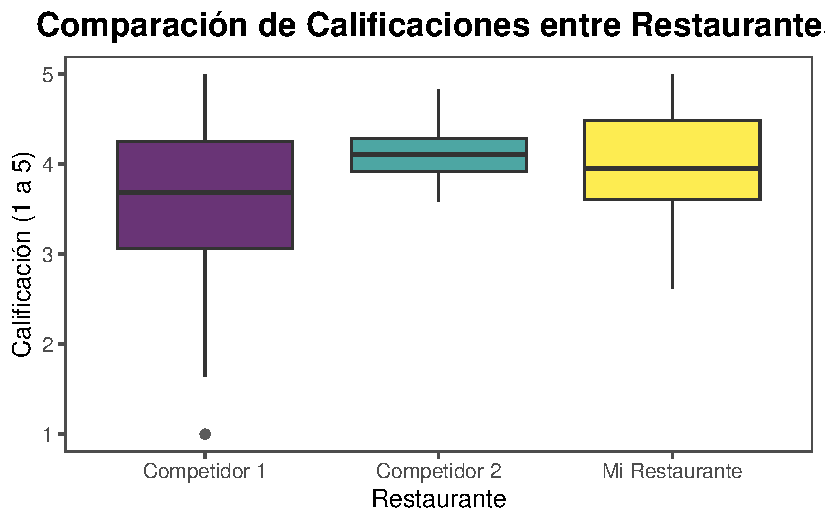
\includegraphics[width=3.64583in,height=\textheight,keepaspectratio]{capitulo3_files/figure-pdf/unnamed-chunk-12-1.pdf}
\end{center}

\section{Medidas de Relación
Lineal}\label{medidas-de-relaciuxf3n-lineal}

Estas nos dicen si dos variables están relacionadas entre sí.

Imagina que además de las calificaciones que dan tus clientes, también
registras cuántas veces visitan tu restaurante al mes. Quieres entender
si estas dos cosas están relacionadas: ¿los clientes que visitan más
tienden a dar mejores calificaciones? ¿O tal vez ocurre lo contrario?

\subsection{Covarianza}\label{covarianza}

La \textbf{covarianza} es una medida que nos indica si dos variables
tienden a subir o bajar juntas.

\begin{itemize}
\tightlist
\item
  Si la covarianza es \textbf{positiva}, significa que cuando una
  variable aumenta, la otra también tiende a aumentar.\\
\item
  Si es \textbf{negativa}, cuando una variable sube, la otra tiende a
  bajar.\\
\item
  Si es cercana a \textbf{cero}, no hay una relación lineal clara entre
  ellas.
\end{itemize}

Sin embargo, la covarianza solo nos dice la dirección de la relación,
pero no qué tan fuerte es, y su valor depende de las unidades de las
variables, lo que dificulta compararla entre diferentes pares de
variables. Es decir, no puedo comparar dos covarianzas de dos variables
distintas.

\subsection{Coeficiente de
Correlación}\label{coeficiente-de-correlaciuxf3n}

Para solucionar esas limitaciones, usamos el \textbf{coeficiente de
correlación}.

Este coeficiente es una versión estandarizada de la covarianza que
siempre toma un valor entre -1 y 1:

\begin{itemize}
\tightlist
\item
  \textbf{1} indica una relación lineal positiva perfecta: a más
  visitas, mejores calificaciones, siempre.\\
\item
  \textbf{-1} indica una relación lineal negativa perfecta: a más
  visitas, peores calificaciones, siempre.\\
\item
  \textbf{0} indica que no hay una relación lineal significativa entre
  las variables.
\end{itemize}

Por ejemplo, un coeficiente de correlación de 0.7 entre visitas y
calificaciones indica una relación positiva fuerte: los clientes que
visitan más suelen estar más satisfechos.

Sin embargo, que haya correlación no implica que una variable
\textbf{cause} la otra, sólo que existe alguna relación la cual incluso
puede ser casualidad no causalidad. Miremos un ejemplo donde correlación
no implica causalidad:

\begin{center}

\includegraphics[width=3.64583in,height=\textheight,keepaspectratio]{img/correlacion_1.png}
\end{center}

\begin{center}
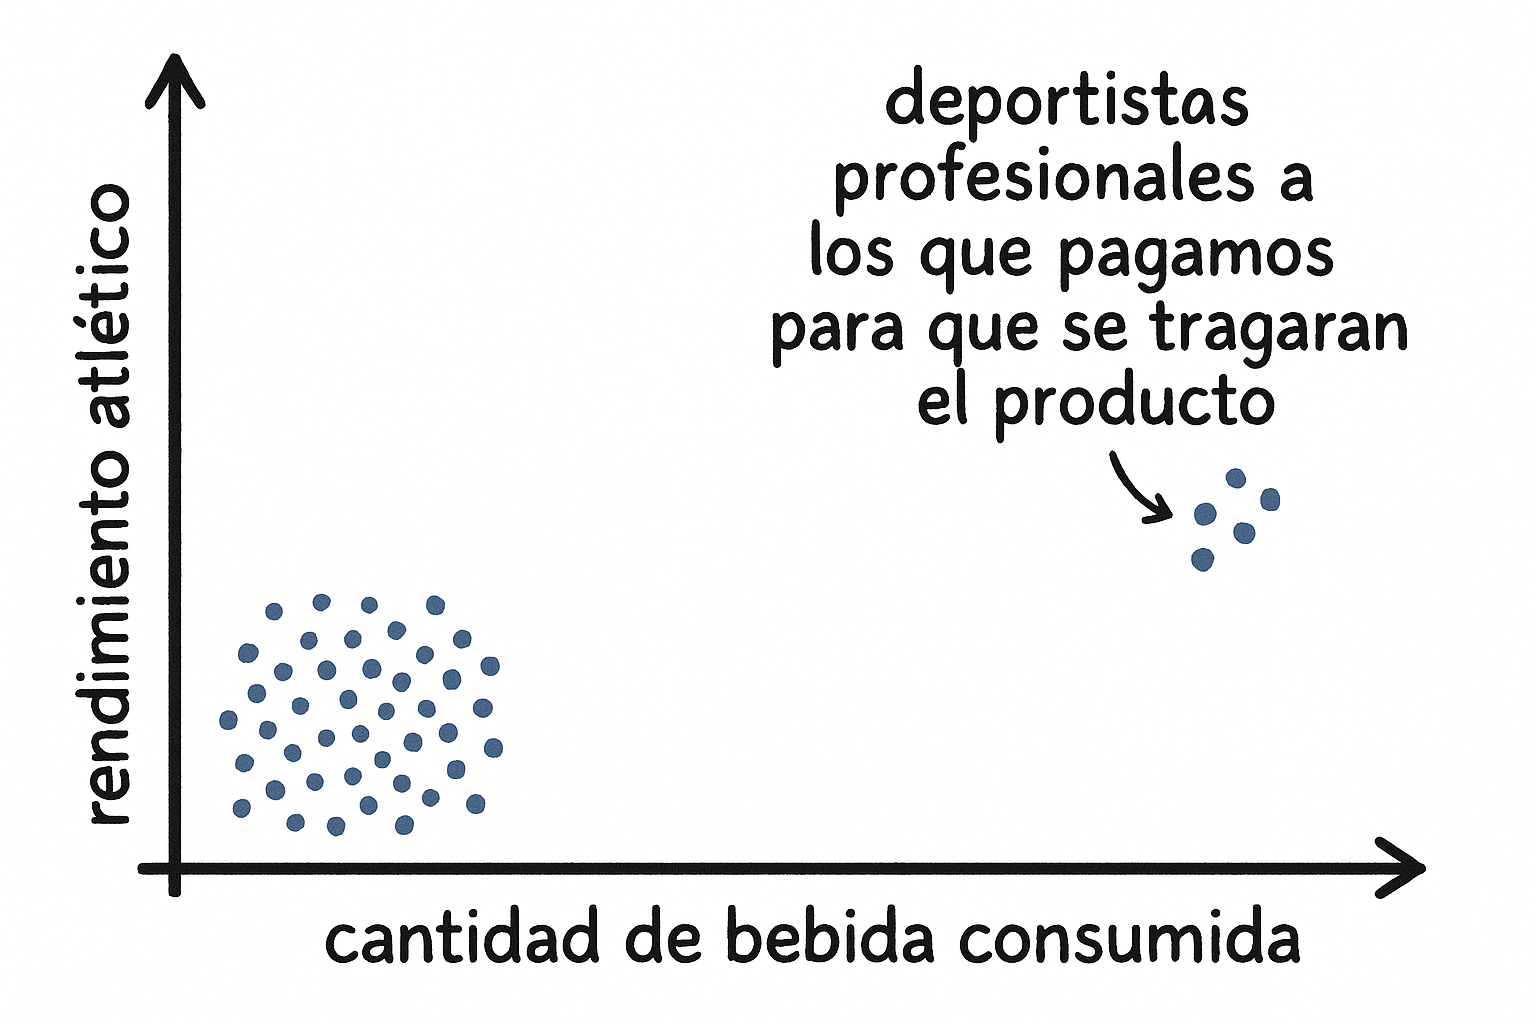
\includegraphics[width=3.64583in,height=\textheight,keepaspectratio]{img/correlacion_2.png}
\end{center}

\bookmarksetup{startatroot}

\chapter{Contando Historias Claras con
Gráficos}\label{contando-historias-claras-con-gruxe1ficos}

Imagina que entras a una librería y tomas un libro por curiosidad. Lo
abres en una página al azar y notas que algo llama inmediatamente tu
atención: un gráfico con colores vibrantes, líneas claras y un mensaje
sencillo de entender. ¿Qué hizo que te fijaras primero en ese gráfico?
Vamos a descubrirlo.

\section{¿Qué es una buena
gráfica?}\label{quuxe9-es-una-buena-gruxe1fica}

Una gráfica efectiva no solo muestra números o barras. Es una
herramienta poderosa que cuenta historias, explica conceptos y revela
información de manera clara y sencilla. Algunas claves importantes para
una buena gráfica son:

\begin{itemize}
\tightlist
\item
  \textbf{Claridad en la rotulación:} Todos los elementos del gráfico
  deben estar claramente identificados.
\item
  \textbf{Sin ornamentación innecesaria:} Menos es más. No necesitas
  adornos que distraigan del mensaje principal.
\item
  \textbf{Uso juicioso del color:} Elige colores que ayuden a resaltar
  lo más importante.
\item
  \textbf{Una historia simple y clara:} El gráfico debe ser fácil de
  entender a simple vista.
\end{itemize}

\section{Cómo leemos gráficos: principios
clave}\label{cuxf3mo-leemos-gruxe1ficos-principios-clave}

Existen cinco principios que describen cómo observamos y entendemos las
gráficas:

\begin{enumerate}
\def\labelenumi{\arabic{enumi}.}
\tightlist
\item
  \textbf{No vamos en orden:} Nuestra vista puede empezar por cualquier
  parte del gráfico. Es posible que no leas el título hasta mucho
  después.
\item
  \textbf{Primero vemos lo que se destaca:} Automáticamente nuestros
  ojos buscan picos, colores intensos, intersecciones o valores
  atípicos.
\item
  \textbf{Vemos solo unas pocas cosas a la vez:} Demasiada información
  puede confundir. Concéntrate en pocos puntos clave.
\item
  \textbf{Buscamos significado y conexiones:} Al ver algo llamativo,
  inmediatamente intentamos entender qué significa.
\item
  \textbf{Nos basamos en convenciones y metáforas:} Interpretamos
  gráficos usando lo que ya conocemos y lo que hemos aprendido antes.
\end{enumerate}

\section{El uso inteligente del
color}\label{el-uso-inteligente-del-color}

Supongamos que quieres mostrar cómo han evolucionado las ventas de
productos electrónicos en una tienda durante el último año. Tienes
información de varias categorías como televisores, teléfonos y
audífonos. ¿Cómo resaltas lo más importante?

\begin{itemize}
\item
  Primero, piensa cuál es la pregunta más importante que debería
  responder tu gráfico. ¿Quizás mostrar que los teléfonos han superado
  ampliamente las ventas de los otros productos?
\item
  Usa un color vibrante como el azul intenso para la categoría principal
  (teléfonos) y usa tonos grises o menos saturados para el resto
  (televisores y audífonos). El contraste inmediatamente enfocará la
  atención hacia los teléfonos, destacando claramente tu punto.
\end{itemize}

\textbf{Consejo práctico:} Haz todo gris excepto lo más importante. El
gris es tu aliado, resaltando por contraste el mensaje central del
gráfico.

\section{Conclusión}\label{conclusiuxf3n}

La próxima vez que diseñes un gráfico, recuerda que estás contando una
historia. Decide qué quieres destacar, usa colores sabiamente y mantén
la claridad y simplicidad. Así, tus lectores no solo verán un gráfico,
sino que comprenderán y recordarán tu mensaje.

\bookmarksetup{startatroot}

\chapter{Intervalos de Confianza y Pruebas de
Hipótesis}\label{intervalos-de-confianza-y-pruebas-de-hipuxf3tesis}

Imagina que eres el gerente de un restaurante que acaba de lanzar un
nuevo plato estrella y quieres saber si a tus clientes les gusta tanto
como esperabas.

Después de varias semanas recogiste las opiniones de algunos clientes:
les pediste que calificaran de 1 a 5 qué tan satisfechos quedaron.

Ya sabes calcular promedios, medianas y varianzas (¡bien hecho hasta
aquí 🎉!), pero surge una nueva pregunta:

\begin{quote}
¿Podemos usar la muestra de clientes que respondieron para decir algo
sobre \textbf{todos} los clientes del restaurante, incluso los que no
alcanzamos a encuestar?
\end{quote}

Aquí entran en juego dos herramientas de la estadística inferencial:
\textbf{los intervalos de confianza} y \textbf{las pruebas de
hipótesis}.

\begin{center}\rule{0.5\linewidth}{0.5pt}\end{center}

\section{Intervalos de Confianza}\label{intervalos-de-confianza}

Imagina que lanzaste un nuevo plato al menú y quieres saber si a los
clientes realmente les gusta. No puedes preguntarle a cada comensal,
pero sí ofreces muestras del plato a algunos clientes y recoges sus
calificaciones. Esas degustaciones te dan una pista, no la verdad
absoluta, sobre la opinión de toda la clientela.

En la mayoría de estudios sucede esto: se toma una muestra y se infiere
información sobre la población total. Esto es porque es muy difícil o
costoso preguntar a todos los clientes.

\begin{figure}[H]

{\centering 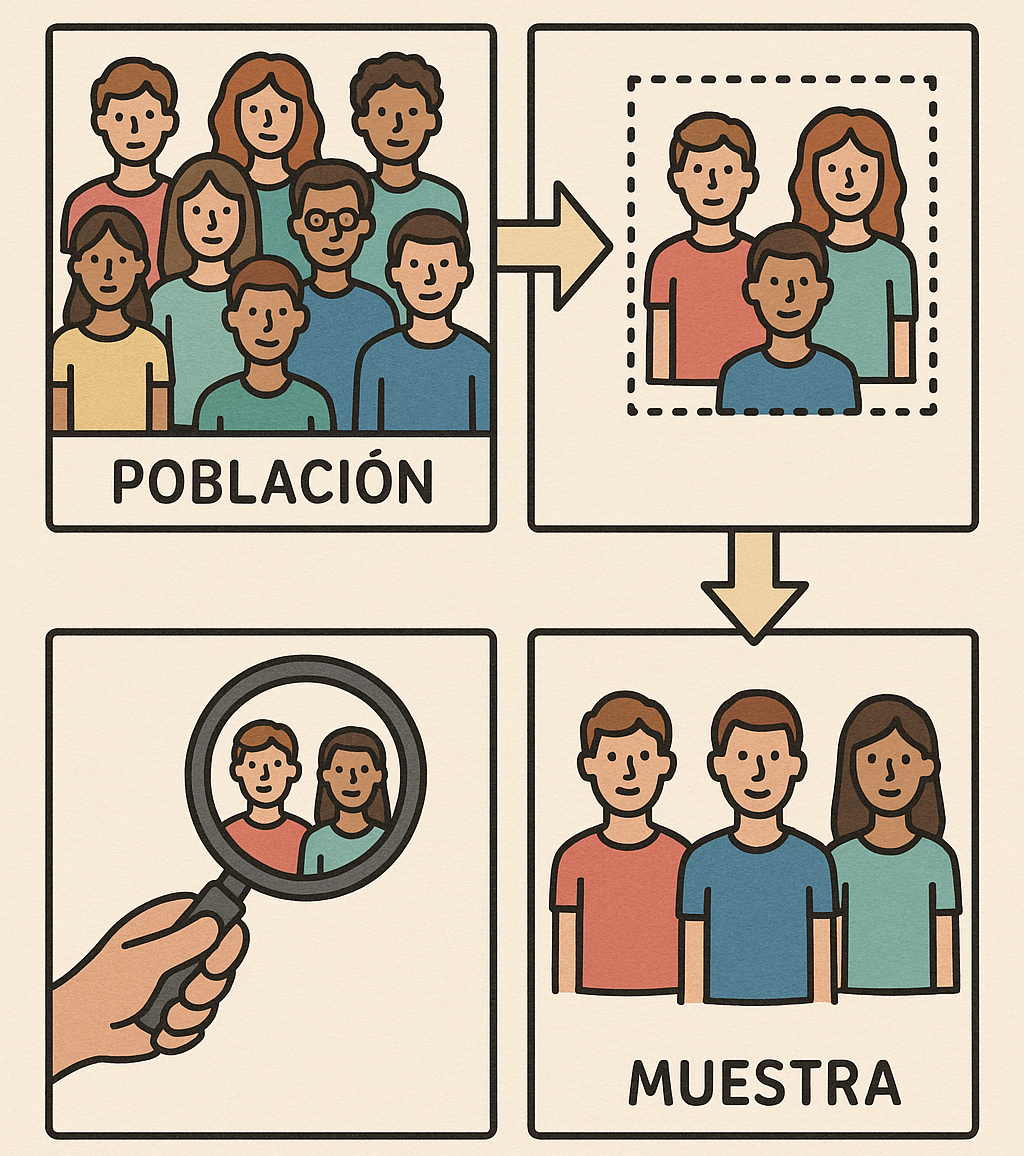
\includegraphics[width=0.4\linewidth,height=\textheight,keepaspectratio]{img/muestra.png}

}

\caption{Población vs muestra}

\end{figure}%

Un intervalo de confianza funciona igual para un parámetro (por ejemplo,
el promedio de satisfacción): parte de la estimación obtenida en la
muestra (la ``degustación'') y le añade y quita un margen de error para
formar un rango plausible. Dos puntos clave para entenderlo
intuitivamente:

\begin{itemize}
\item
  Interpretación práctica: cuando hablamos de un ``IC 95\%'' describimos
  el método: si repitieras el muestreo muchas veces y construyeras
  intervalos con el mismo procedimiento, alrededor del 95\% de esos
  intervalos incluirían el valor verdadero desconocido. No quiere decir
  que exista un 95\% de probabilidad de que este intervalo concreto lo
  contenga; el valor real es fijo y lo que cambia es el intervalo que
  construimos.
\item
  \emph{¿Qué influye en el ancho del intervalo?}
\end{itemize}

\begin{enumerate}
\def\labelenumi{\arabic{enumi}.}
\tightlist
\item
  La dispersión de las calificaciones --- más variabilidad → intervalos
  más anchos.
\item
  El tamaño de la muestra --- más clientes encuestados → intervalos más
  estrechos.
\item
  El nivel de confianza elegido --- mayor confianza → intervalos más
  amplios.
\end{enumerate}

Visualiza esto como elegir el tamaño de la degustación y el margen de
seguridad alrededor de tu estimación: si usas un margen muy amplio te
aseguras de cubrir el valor verdadero pero pierdes precisión; si eliges
un margen muy estrecho ganas precisión pero aumentas la probabilidad de
equivocarte.

En resumen: un intervalo de confianza te ofrece un rango razonable para
la media poblacional (por ejemplo, la satisfacción real de todos los
clientes), acompañado de una medida explícita de cuánta confianza te da
ese procedimiento si lo repitieras muchas veces.

\subsection{¿Cómo se construye?}\label{cuxf3mo-se-construye}

El intervalo de confianza toma el promedio de tu muestra y le agrega un
``margen de error''.

Ese margen depende de dos cosas:\\
- Qué tan variable son las opiniones (la desviación estándar).\\
- Cuántos clientes alcanzaste a encuestar (el tamaño de la muestra).

\begin{tcolorbox}[enhanced jigsaw, toptitle=1mm, opacitybacktitle=0.6, leftrule=.75mm, arc=.35mm, title=\textcolor{quarto-callout-tip-color}{\faLightbulb}\hspace{0.5em}{Fórmula del intervalo}, colback=white, bottomrule=.15mm, colbacktitle=quarto-callout-tip-color!10!white, opacityback=0, bottomtitle=1mm, breakable, rightrule=.15mm, coltitle=black, left=2mm, titlerule=0mm, colframe=quarto-callout-tip-color-frame, toprule=.15mm]

\[
IC_{95\%} = \bar{x} \pm Z \cdot \frac{s}{\sqrt{n}}
\]

\begin{itemize}
\tightlist
\item
  ( \(\bar{x}\) ): promedio de la muestra\\
\item
  ( \(s\) ): variabilidad de las opiniones\\
\item
  ( \(n\) ): número de clientes encuestados\\
\item
  ( \(Z\) ): un número fijo que depende del nivel de confianza (1.96
  para 95\%)\\
\end{itemize}

\end{tcolorbox}

\subsection{Ejemplo del restaurante}\label{ejemplo-del-restaurante}

Encuestaste a \textbf{50 clientes}.\\
El promedio de satisfacción fue \textbf{4.2} y la desviación estándar
\textbf{0.8}.

\[
IC_{95\%} = 4.2 \pm 1.96 \cdot \frac{0.8}{\sqrt{50}} \approx (4.0,\;4.4)
\]

Esto significa que, aunque no hablamos con todos los clientes, podemos
decir con un 95\% de confianza que la satisfacción promedio real de
\emph{todos} los comensales está entre \textbf{4.0 y 4.4}.

\begin{tcolorbox}[enhanced jigsaw, toptitle=1mm, opacitybacktitle=0.6, leftrule=.75mm, arc=.35mm, title=\textcolor{quarto-callout-tip-color}{\faLightbulb}\hspace{0.5em}{Tip}, colback=white, bottomrule=.15mm, colbacktitle=quarto-callout-tip-color!10!white, opacityback=0, bottomtitle=1mm, breakable, rightrule=.15mm, coltitle=black, left=2mm, titlerule=0mm, colframe=quarto-callout-tip-color-frame, toprule=.15mm]

\textbf{En otras palabras un intervalo de confianza dice:}

\textbf{No estoy 100\% seguro de la cifra exacta, pero tengo un rango
muy confiable donde debe estar el promedio verdadero si pudiéramos
preguntar a todos los clientes.}

\end{tcolorbox}

\begin{center}\rule{0.5\linewidth}{0.5pt}\end{center}

\section{Pruebas de Hipótesis}\label{pruebas-de-hipuxf3tesis}

Ahora imagina otra situación: tTu socio del restaurante es un poco
escéptico y te dice:\\
\textgreater{} ``\emph{Yo creo que los clientes nos califican, en
promedio, con 4. Nada más}.''

Tú, viendo tus datos, sospechas que en realidad el promedio es
\textbf{mayor} a 4.

¿Cómo decidir quién tiene razón?

Aquí usamos una \textbf{prueba de hipótesis}. Es como un juicio
estadístico:

\begin{itemize}
\tightlist
\item
  Partimos de la \textbf{hipótesis nula (H₀)}: lo que asumimos de
  entrada.\\
\item
  Luego vemos si hay suficiente evidencia en la muestra para rechazarla
  y quedarnos con la \textbf{hipótesis alternativa (H₁)}.
\end{itemize}

\subsection{Pasos de la prueba}\label{pasos-de-la-prueba}

\begin{enumerate}
\def\labelenumi{\arabic{enumi}.}
\tightlist
\item
  \textbf{Plantear hipótesis}

  \begin{itemize}
  \tightlist
  \item
    H₀: \(\mu = 4\) (los clientes en promedio califican con 4).\\
  \item
    H₁: \(\mu > 4\) (los clientes en promedio califican con más de 4).
  \end{itemize}
\item
  \textbf{Elegir un nivel de significancia}

  \begin{itemize}
  \tightlist
  \item
    Normalmente usamos 5\% (α = 0.05).\\
  \item
    Significa que aceptamos un 5\% de riesgo de equivocarnos al rechazar
    H₀.
  \end{itemize}
\item
  \textbf{Calcular el p-valor y tomar la decisión}
\end{enumerate}

\begin{itemize}
\tightlist
\item
  Usamos el sofware de preferencia para calcular la prueba t y obtener
  el p-valor.
\item
  Si \(p < \alpha\) (por ejemplo \(\alpha=0.05\)) rechazamos H₀; si
  \(p \ge \alpha\) no rechazamos H₀.
\end{itemize}

\begin{tcolorbox}[enhanced jigsaw, toptitle=1mm, opacitybacktitle=0.6, leftrule=.75mm, arc=.35mm, title=\textcolor{quarto-callout-note-color}{\faInfo}\hspace{0.5em}{Nota}, colback=white, bottomrule=.15mm, colbacktitle=quarto-callout-note-color!10!white, opacityback=0, bottomtitle=1mm, breakable, rightrule=.15mm, coltitle=black, left=2mm, titlerule=0mm, colframe=quarto-callout-note-color-frame, toprule=.15mm]

Nota práctica: no necesitas calcular el p-valor a mano

La mayoría de los paquetes estadísticos calculan y reportan el p-valor
automáticamente:

\begin{itemize}
\tightlist
\item
  En R: \texttt{t.test(x,\ mu\ =\ 4)} devuelve la estadística, el
  p-valor y el intervalo de confianza.
\item
  En Python (SciPy): \texttt{scipy.stats.ttest\_1samp(x,\ 4)} devuelve
  la estadística t y el p-valor.
\item
  En Excel: la herramienta de análisis de datos o la función T.TEST
  reportan p-valores.
\end{itemize}

Lo importante es entender qué mide el p-valor y cómo interpretarlo, no
hacer el cálculo manual cada vez.

\end{tcolorbox}

\begin{center}\rule{0.5\linewidth}{0.5pt}\end{center}

\subsection{Ejemplo del restaurante}\label{ejemplo-del-restaurante-1}

Con los datos de antes (\(\bar{x}=4.2,\; s=0.8,\; n=50\)) podemos usar
el concepto de \emph{p-valor} para decidir si rechazar H₀.

Intuitivamente, el p-valor responde a la pregunta: si la hipótesis nula
fuera cierta (es decir, si no hubiera diferencia real y el verdadero
promedio fuera 4), ¿qué probabilidad hay de obtener un resultado igual o
más extremo que el observado? Para explicarlo paso a paso:

\begin{enumerate}
\def\labelenumi{\arabic{enumi}.}
\tightlist
\item
  Supón por un momento que estamos persiguiendo un golpe de suerte: la
  hipótesis nula es verdadera (p.~ej. el nuevo plato no cambia la
  satisfacción, la media es 4).
\item
  Imagina la distribución de todos los resultados posibles que podríamos
  haber obtenido al repetir el experimento muchas veces bajo H₀. La
  mayoría serían resultados modestos y no llamativos; unos pocos serían
  flukes (suertes raras) que parecen indicar un efecto.
\item
  Ubica nuestro resultado real dentro de esa distribución: el p-valor es
  la fracción de resultados bajo H₀ que serían tan o más extremos que el
  nuestro.
\end{enumerate}

Un p-valor pequeño (por ejemplo, 0.03) significa que sólo un pequeño
porcentaje de resultados falsos serían tan espectaculares; esa rareza
sugiere que tal vez no sea un fluke y que haya un efecto real.

Aplicando esto a nuestros datos, el p-valor unilateral resultante es
aproximadamente \(p \approx 0.038\) (≈3.8\%). Es decir: si de verdad el
promedio fuera 4, sólo en \textasciitilde3.8\% de las muestras
obtendríamos un resultado tan extremo por azar.

Regla de decisión: si \(p < \alpha\) (por ejemplo \(\alpha=0.05\)),
rechazamos H₀. Aquí \(0.038 < 0.05\), por lo que la evidencia es lo
suficientemente fuerte para rechazar H₀.

\begin{tcolorbox}[enhanced jigsaw, toptitle=1mm, opacitybacktitle=0.6, leftrule=.75mm, arc=.35mm, title=\textcolor{quarto-callout-tip-color}{\faLightbulb}\hspace{0.5em}{Veredicto}, colback=white, bottomrule=.15mm, colbacktitle=quarto-callout-tip-color!10!white, opacityback=0, bottomtitle=1mm, breakable, rightrule=.15mm, coltitle=black, left=2mm, titlerule=0mm, colframe=quarto-callout-tip-color-frame, toprule=.15mm]

Rechazamos H₀.\\
Podemos afirmar que, en promedio, tus clientes están \textbf{más
satisfechos} que el 4 que sospechaba tu socio.

\end{tcolorbox}

\begin{center}\rule{0.5\linewidth}{0.5pt}\end{center}

\begin{tcolorbox}[enhanced jigsaw, toptitle=1mm, opacitybacktitle=0.6, leftrule=.75mm, arc=.35mm, title=\textcolor{quarto-callout-note-color}{\faInfo}\hspace{0.5em}{Nota}, colback=white, bottomrule=.15mm, colbacktitle=quarto-callout-note-color!10!white, opacityback=0, bottomtitle=1mm, breakable, rightrule=.15mm, coltitle=black, left=2mm, titlerule=0mm, colframe=quarto-callout-note-color-frame, toprule=.15mm]

Importante --- ``rechazar'' vs ``aceptar'' H₀

En estadística decimos que \emph{rechazamos} la hipótesis nula o
\emph{no la rechazamos}, pero no la \emph{aceptamos} como verdadera.
Intuitivamente es así porque la prueba está diseñada para buscar
evidencia en contra de H₀: si la evidencia es fuerte, la descartamos; si
no lo es, simplemente no tenemos base para descartarla.

Piensa en un juicio: la ausencia de pruebas suficientes para condenar no
es una prueba de inocencia absoluta. Del mismo modo, que los datos no
permitan rechazar H₀ puede deberse a que H₀ es plausible \emph{o} a que
la muestra es pequeña o el test no tiene poder suficiente para detectar
la diferencia (error tipo II). Por eso los científicos hablan de ``no
rechazar'' y complementan con tamaño del efecto y poder del estudio.

\end{tcolorbox}

\section{Comparando dos grupos: ¿de verdad son
diferentes?}\label{comparando-dos-grupos-de-verdad-son-diferentes}

\begin{quote}
\textbf{Idea clave:} tener dos medias con valores distintos \textbf{no}
implica automáticamente que sean \textbf{estadísticamente diferentes}.\\
Una diferencia pequeña puede deberse al azar de a quiénes encuestamos,
especialmente si las muestras son pequeñas o muy variables.
\end{quote}

Imagina que tu restaurante tiene \textbf{dos sedes}:

\begin{itemize}
\tightlist
\item
  \textbf{Sede Norte}: acabas de implementar una capacitación en
  servicio.
\item
  \textbf{Sede Sur}: aún no (sirve como comparación).
\end{itemize}

Encuestas la satisfacción (1 a 5) de clientes en ambas sedes y obtienes:

\begin{itemize}
\tightlist
\item
  \textbf{Norte:} (\(\bar{x}_N = 4.3\)), (\(s_N = 0.7\)),
  (\(n_N = 40\))\\
\item
  \textbf{Sur:} (\(\bar{x}_S = 4.1\)), (\(s_S = 0.9\)), (\(n_S = 45\))
\end{itemize}

A simple vista \textbf{4.3 vs 4.1} luce mejor en Norte, ¿pero alcanza
para concluir que la capacitación \textbf{elevó} la satisfacción? Vamos
paso a paso.

\subsection{Prueba de dos medias (grupos
independientes)}\label{prueba-de-dos-medias-grupos-independientes}

Cuando las personas encuestadas en un grupo \textbf{no} son las mismas
del otro grupo (clientes distintos en cada sede), usamos una prueba de
dos muestras \textbf{independientes}. Por defecto, usa la versión
\textbf{Welch} (no asume varianzas iguales).

\textbf{Hipótesis (bilateral):}

\begin{itemize}
\item
  (\(H_0:\ \mu_N - \mu_S = 0\)) (no hay diferencia real)
\item
  (\(H_1:\ \mu_N - \mu_S \neq 0\)) (sí hay diferencia)
\end{itemize}

Para un nivel de significancia (\(\alpha=0.05\)) (bilateral), el
\textbf{p-valor} bilateral es (\(\approx 0.25\)): no hay evidencia
suficiente para afirmar que las medias difieren. \textbf{No rechazamos
(\(H_0\)).}

\textbf{Intervalo de confianza (95\%) para (\(\mu_N - \mu_S\)):} \[
(0.2) \pm 1.99 \times 0.174 \;\approx\; (-0.15,\; 0.55)
\] Como el \textbf{0} está dentro del intervalo, la diferencia podría
ser nula.

\begin{tcolorbox}[enhanced jigsaw, toptitle=1mm, opacitybacktitle=0.6, leftrule=.75mm, arc=.35mm, title=\textcolor{quarto-callout-tip-color}{\faLightbulb}\hspace{0.5em}{Lectura práctica}, colback=white, bottomrule=.15mm, colbacktitle=quarto-callout-tip-color!10!white, opacityback=0, bottomtitle=1mm, breakable, rightrule=.15mm, coltitle=black, left=2mm, titlerule=0mm, colframe=quarto-callout-tip-color-frame, toprule=.15mm]

\begin{itemize}
\tightlist
\item
  Que la media de Norte sea 4.3 y la de Sur 4.1 \textbf{no basta} para
  declarar una mejora real.
\item
  Con esta evidencia, \textbf{no podemos asegurar} que la capacitación
  subió la satisfacción; necesitamos más datos o un efecto más grande.
\end{itemize}

\end{tcolorbox}

\subsubsection{Decidir unilateral vs
bilateral}\label{decidir-unilateral-vs-bilateral}

\begin{itemize}
\tightlist
\item
  \textbf{Bilateral ((\(\neq\)))} cuando buscas \emph{cualquier}
  diferencia.\\
\item
  \textbf{Unilateral (\textgreater{} o \textless)} solo si
  \textbf{antes} de ver los datos** tienes una hipótesis direccional
  clara (p.~ej., ``la capacitación \textbf{aumenta} la satisfacción'').
\end{itemize}

\subsection{¿Y si las muestras son las mismas personas? (Prueba
pareada)}\label{y-si-las-muestras-son-las-mismas-personas-prueba-pareada}

Otra historia típica del restaurante: encuestas a \textbf{los mismos
clientes} \textbf{antes} y \textbf{después} de la capacitación en la
\textbf{Sede Norte}.

Aquí cada persona funciona como su \textbf{propio control} → usamos una
prueba \textbf{pareada} (de medias de \textbf{diferencias}).

\begin{itemize}
\tightlist
\item
  Define (\(d_i = \text{(después)} - \text{(antes)}\)).\\
\item
  Hipótesis:

  \begin{itemize}
  \tightlist
  \item
    (\(H_0: \mu_d = 0\)) (en promedio, no cambia)
  \item
    (\(H_1: \mu_d > 0\)) (en promedio, mejora)
  \end{itemize}
\end{itemize}

\textbf{Ejemplo:} 30 clientes habituales,\\
(\(\bar{d} = 0.25\)) puntos, (\(s_d = 0.50\)).

Con (\(\alpha=0.05\)) unilateral, esto \textbf{sí} es significativo (p
(\(\approx 0.01\))).

\textbf{Interpretación:} en la \emph{misma} sede y \emph{mismas}
personas, la satisfacción \textbf{aumentó} tras la capacitación.

\begin{tcolorbox}[enhanced jigsaw, toptitle=1mm, opacitybacktitle=0.6, leftrule=.75mm, arc=.35mm, title=\textcolor{quarto-callout-important-color}{\faExclamation}\hspace{0.5em}{¿Independientes o pareadas?}, colback=white, bottomrule=.15mm, colbacktitle=quarto-callout-important-color!10!white, opacityback=0, bottomtitle=1mm, breakable, rightrule=.15mm, coltitle=black, left=2mm, titlerule=0mm, colframe=quarto-callout-important-color-frame, toprule=.15mm]

\begin{itemize}
\tightlist
\item
  \textbf{Independientes:} Norte vs Sur (clientes \textbf{distintos} en
  cada sede).\\
\item
  \textbf{Pareadas:} Antes vs Después en \textbf{la misma} sede y
  \textbf{mismas} personas.
\end{itemize}

\end{tcolorbox}

\begin{center}\rule{0.5\linewidth}{0.5pt}\end{center}

\subsection{Checklist rápido para comparar dos
medias}\label{checklist-ruxe1pido-para-comparar-dos-medias}

\begin{enumerate}
\def\labelenumi{\arabic{enumi}.}
\tightlist
\item
  \textbf{Escenario:}

  \begin{itemize}
  \tightlist
  \item
    ¿Independientes (Norte vs Sur) o Pareadas (Antes vs Después)?
  \end{itemize}
\item
  \textbf{Dirección de la hipótesis:}

  \begin{itemize}
  \tightlist
  \item
    ¿Buscas \emph{cualquier} diferencia (bilateral) o una mejora
    concreta (unilateral)?
  \end{itemize}
\end{enumerate}

\begin{tcolorbox}[enhanced jigsaw, toptitle=1mm, opacitybacktitle=0.6, leftrule=.75mm, arc=.35mm, title=\textcolor{quarto-callout-tip-color}{\faLightbulb}\hspace{0.5em}{Estadísticamente vs.~prácticamente significativo}, colback=white, bottomrule=.15mm, colbacktitle=quarto-callout-tip-color!10!white, opacityback=0, bottomtitle=1mm, breakable, rightrule=.15mm, coltitle=black, left=2mm, titlerule=0mm, colframe=quarto-callout-tip-color-frame, toprule=.15mm]

Un resultado puede ser estadísticamente significativo pero \textbf{poco
relevante} en la práctica (p.~ej., mejora de 0.05 puntos en satisfacción
con miles de encuestas).\\
En decisiones de negocio, combina el resultado estadístico con el
\textbf{impacto real}.

\end{tcolorbox}

\subsection{En resumen}\label{en-resumen}

\begin{itemize}
\item
  Los \textbf{intervalos de confianza} son como dar un rango plausible
  para la verdadera satisfacción de todos los clientes.
\item
  Las \textbf{pruebas de hipótesis} son como un juicio: partimos de una
  suposición y vemos si la evidencia la sostiene o la derrumba.
\end{itemize}

Ambas herramientas permiten ir más allá de describir lo que vemos en los
datos: nos ayudan a \textbf{inferir} sobre toda la población de clientes
del restaurante.

\bookmarksetup{startatroot}

\chapter{Descubriendo Patrones con Regresión
Lineal}\label{descubriendo-patrones-con-regresiuxf3n-lineal}

\begin{center}
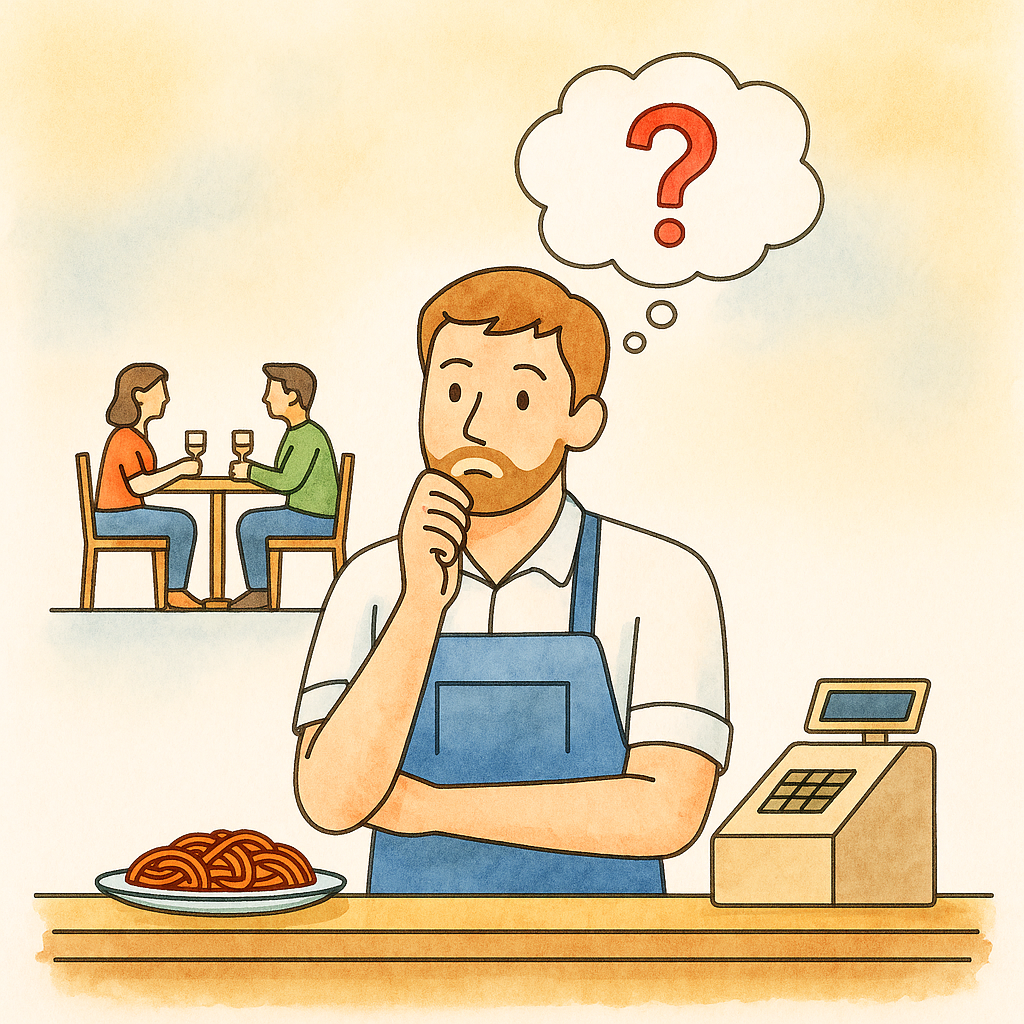
\includegraphics[width=0.6\linewidth,height=\textheight,keepaspectratio]{img/reg_1.png}
\end{center}

Imagina que eres dueño de un restaurante 🍝.\\
Cada día recibes clientes, vendes platos y al final de la semana te
preguntas:

\begin{quote}
\textbf{¿Qué hace que mis ventas suban o bajen?}\\
¿Será el precio de los platos, la inversión en publicidad, o quizá los
fines de semana festivos?
\end{quote}

Aquí entra en acción la \textbf{regresión lineal}, una herramienta que
nos ayuda a descubrir patrones escondidos en los datos.

\section{Una primera pista con la Regresión
Simple}\label{una-primera-pista-con-la-regresiuxf3n-simple}

Empecemos simple: ¿qué pasa con tus ventas y el precio del menú?

Si anotas tus datos semana a semana y los pones en un gráfico como el de
abajo, notarás que cuando el precio sube, las ventas tienden a bajar. La
regresión lineal traza la \textbf{mejor línea recta} que explica esa
relación.

\begin{figure}[H]

{\centering 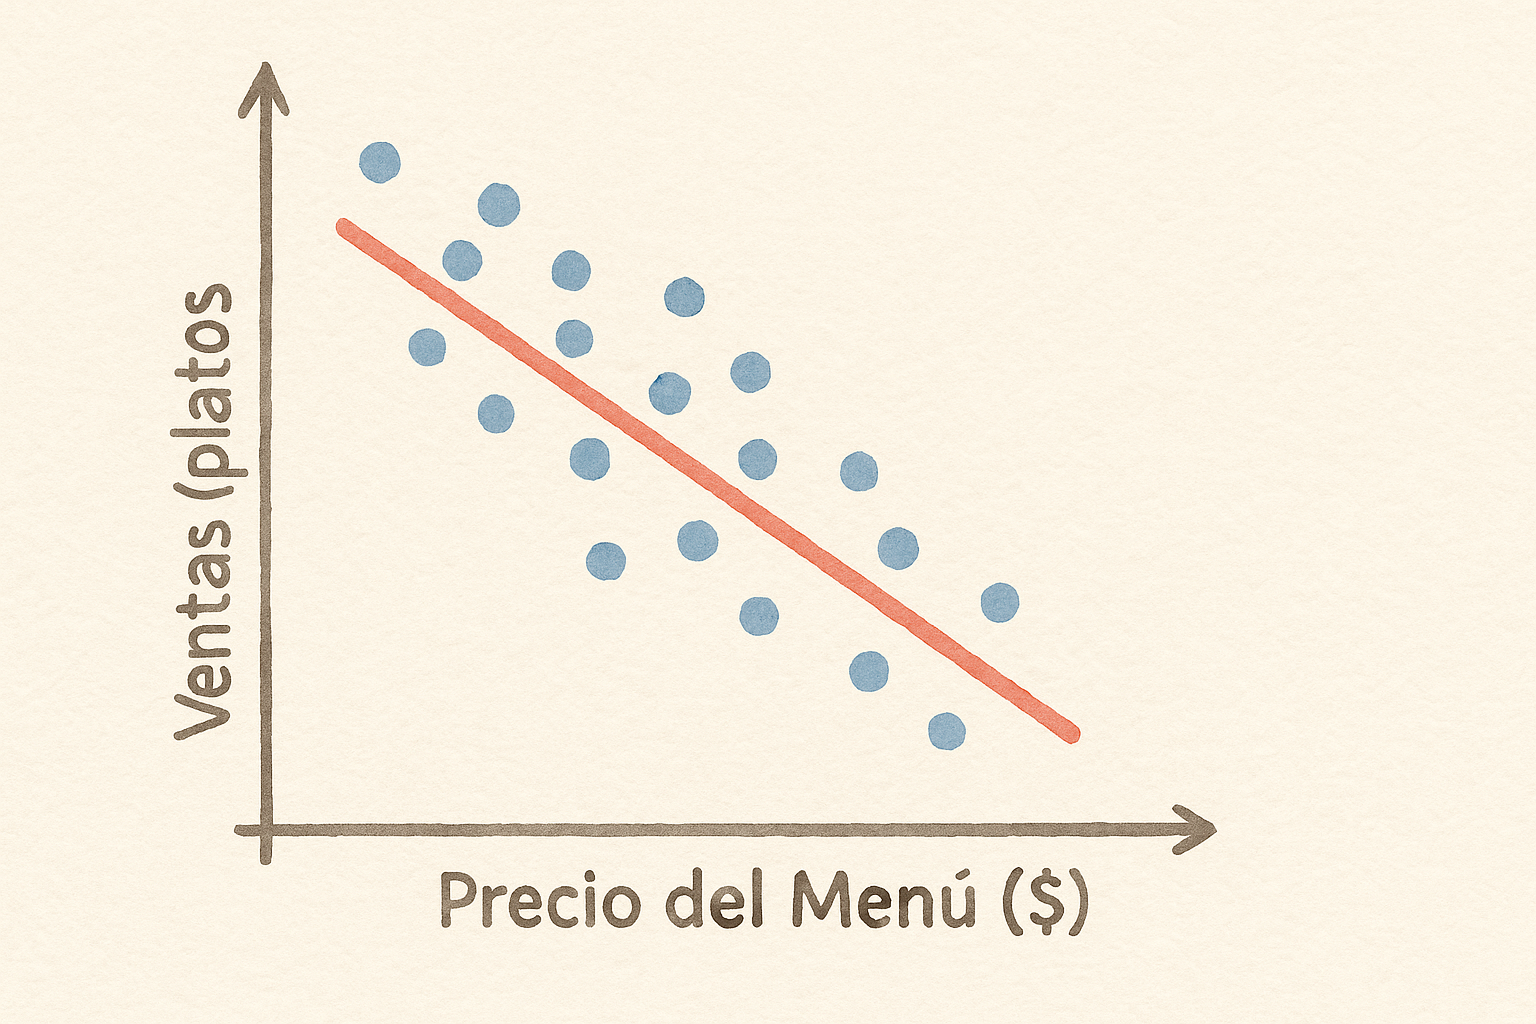
\includegraphics[width=0.6\linewidth,height=\textheight,keepaspectratio]{img/reg_2.png}

}

\caption{Gráfico de dispersión ventas vs.~precio}

\end{figure}%

La ecuación que representa la línea roja de ese gráfico se ve así:

\[
Ventas = b_0 + b_1 \times Precio + \varepsilon
\]

\begin{itemize}
\tightlist
\item
  \textbf{\(b_0\)}: el punto de partida (ventas cuando el precio es
  cero, aunque no sea realista vender gratis 🍕).\\
\item
  \textbf{\(b_1\)}: la \emph{pendiente}; cuánto cambian las ventas si
  subes el precio en una unidad.\\
\item
  \textbf{\(\varepsilon\)}: el ruido que la línea no puede explicar
  (clima, humor del chef, partidos de fútbol, etc.).
\end{itemize}

👉 Si el modelo encuentra que:

\[
\hat{Ventas} = 500 - 25 \times Precio
\]

significa que por cada \$1 más en el precio, \textbf{pierdes 25 platos
vendidos en promedio}. ¡Cuidado con pasarte de caro!

\section{¿Es realmente importante mi coeficiente? (significancia
estadística)}\label{es-realmente-importante-mi-coeficiente-significancia-estaduxedstica}

Hasta ahora vimos que un coeficiente \(b_1\) nos dice cómo cambia \(Y\)
cuando \(X\) sube una unidad.

Pero la gran pregunta es: \textbf{¿podemos confiar en que ese efecto no
apareció solo por azar?}

Aquí entran las \textbf{pruebas de hipótesis} que estudiamos el capítulo
anterior.

\subsection{El planteamiento}\label{el-planteamiento}

\begin{itemize}
\tightlist
\item
  \textbf{Hipótesis nula (\(H_0\))}: el coeficiente es igual a 0.\\
  \textgreater{} Es decir, que la variable no tiene efecto real en las
  ventas.\\
\item
  \textbf{Hipótesis alternativa (\(H_1\))}: el coeficiente es diferente
  de 0.\\
  \textgreater{} Que sí existe un impacto real.
\end{itemize}

Para saber si tu coeficiente es realmente significativo, puedes usar el
valor p (p-value). Este valor te dice la probabilidad de que el
coeficiente sea cero (es decir, que no tenga efecto).

\begin{tcolorbox}[enhanced jigsaw, toptitle=1mm, opacitybacktitle=0.6, leftrule=.75mm, arc=.35mm, title=\textcolor{quarto-callout-note-color}{\faInfo}\hspace{0.5em}{Prueba de significancia estadística}, colback=white, bottomrule=.15mm, colbacktitle=quarto-callout-note-color!10!white, opacityback=0, bottomtitle=1mm, breakable, rightrule=.15mm, coltitle=black, left=2mm, titlerule=0mm, colframe=quarto-callout-note-color-frame, toprule=.15mm]

\begin{itemize}
\tightlist
\item
  Si el valor p es menor que 0.05, puedes decir que el coeficiente es
  \textbf{significativo}. Esto significa que hay evidencia suficiente
  para afirmar que el precio sí afecta las ventas.
\item
  Si el valor p es mayor que 0.05, no puedes rechazar la hipótesis nula
  de que el coeficiente es cero. En otras palabras, no hay suficiente
  evidencia para afirmar que el precio afecta las ventas.
\end{itemize}

\end{tcolorbox}

\subsection{Ejemplo de restaurante 🍝}\label{ejemplo-de-restaurante}

Supongamos que obtienes un nuevo modelo al recoger más datos:

\[
\hat{Ventas} = 400 - 20 \times Precio + 60 \times Publicidad
\]

\begin{itemize}
\tightlist
\item
  El coeficiente de \textbf{Precio = -20} sugiere que subir \$1 reduce
  20 platos vendidos.\\
\item
  Pero, ¿y si esa relación negativa se debe solo a la casualidad en tus
  datos?
\end{itemize}

\subsection{La prueba}\label{la-prueba}

El software (R, Excel, Stata, etc.) hace un \textbf{test t} que compara
el valor del coeficiente con la variabilidad de los datos.\\
De ahí sale un número mágico: el \textbf{p-valor}.

\begin{itemize}
\tightlist
\item
  Si el \textbf{p-valor \textless{} 0.05}, rechazamos la hipótesis
  nula.\\
  \textgreater{} Concluimos que el efecto es significativo: el precio
  \emph{sí afecta} las ventas.\\
\item
  Si el \textbf{p-valor ≥ 0.05}, no tenemos suficiente evidencia.\\
  \textgreater{} No podemos asegurar que el precio influya: podría ser
  puro ruido.
\end{itemize}

\subsection{La moraleja}\label{la-moraleja}

Un coeficiente puede verse grande o pequeño, positivo o negativo, pero
lo crucial es saber si es \textbf{estadísticamente diferente de cero}.\\
Solo así podemos decir con confianza que esa variable explica parte de
la historia de nuestros datos.

👉 En negocios, esto significa que antes de tomar decisiones (subir
precios, invertir en publicidad, lanzar una promo) debemos asegurarnos
de que los efectos que vemos no sean simplemente coincidencias.

\section{Midiendo qué tan bien funciona mi
regresión}\label{midiendo-quuxe9-tan-bien-funciona-mi-regresiuxf3n}

No basta con tener la línea (regresión), también queremos saber
\textbf{qué tan buena es}.

Para eso usamos el famoso \textbf{\(R^2\)}, también llamado coeficiente
de determinación:

\begin{itemize}
\tightlist
\item
  Si \(R^2 = 0.8\), entonces el 80\% de las variaciones en ventas se
  explican solo con el precio.\\
\item
  El 20\% restante\ldots{} bueno, puede ser el clima, la competencia, o
  ese influencer foodie que llegó sin avisar 📸.
\end{itemize}

Si \(R^2 = 0\), tu modelo no explica nada: sería como decir que el
precio no tiene relación alguna con las ventas, y que lo único que
podrías hacer es mirar el promedio de todas las semanas.

Si \(R^2 = 1\), tu modelo explica todo: las ventas estarían
perfectamente determinadas por el precio, sin misterios, sin azar, sin
sorpresas (lo cual rara vez pasa en la vida real).

\begin{tcolorbox}[enhanced jigsaw, toptitle=1mm, opacitybacktitle=0.6, leftrule=.75mm, arc=.35mm, title=\textcolor{quarto-callout-tip-color}{\faLightbulb}\hspace{0.5em}{Tip}, colback=white, bottomrule=.15mm, colbacktitle=quarto-callout-tip-color!10!white, opacityback=0, bottomtitle=1mm, breakable, rightrule=.15mm, coltitle=black, left=2mm, titlerule=0mm, colframe=quarto-callout-tip-color-frame, toprule=.15mm]

Piensa en \(R^2\) como un termómetro de confianza: te dice qué tan buena
es tu línea de regresión para capturar la historia detrás de tus datos.
No es perfecto, pero sí es una brújula que te orienta sobre cuánto
puedes fiarte de tu modelo para explicar lo que ves.

\end{tcolorbox}

\section{Sumando más ingredientes: la Regresión
Múltiple}\label{sumando-muxe1s-ingredientes-la-regresiuxf3n-muxfaltiple}

En la vida real, tus ventas no dependen solo del precio.\\
En tu restaurante también influyen otros ``ingredientes'' del negocio:

\begin{itemize}
\tightlist
\item
  el \textbf{precio} del menú,\\
\item
  el \textbf{dinero invertido en publicidad},\\
\item
  y si fue o no una \textbf{semana festiva}.
\end{itemize}

La regresión múltiple nos permite poner todos esos factores en la misma
receta estadística.Supongamos que tus datos arrojan:

\[
\hat{Ventas} = 400 - 20 \times Precio + 60 \times Publicidad + 15 \times Festivo
\]

Interpretación:\\
- Cada \$1 más en el precio reduce en promedio 20 platos vendidos.\\
- Cada \$100 en publicidad aumentan las ventas en 60 platos.\\
- Si es semana festiva, se venden 15 platos extra aunque no cambie nada
más.

\begin{tcolorbox}[enhanced jigsaw, toptitle=1mm, opacitybacktitle=0.6, leftrule=.75mm, arc=.35mm, title=\textcolor{quarto-callout-tip-color}{\faLightbulb}\hspace{0.5em}{Tip}, colback=white, bottomrule=.15mm, colbacktitle=quarto-callout-tip-color!10!white, opacityback=0, bottomtitle=1mm, breakable, rightrule=.15mm, coltitle=black, left=2mm, titlerule=0mm, colframe=quarto-callout-tip-color-frame, toprule=.15mm]

Plantilla de interpretación (ceteris paribus): significa que por cada
unidad que aumente \textbf{variable}, la \textbf{variable dependiente}
cambia en promedio \textbf{coeficiente} unidades, manteniendo constantes
las demás variables.

Ejemplo: por cada \$1 que aumenta el precio, las ventas semanales
disminuyen en promedio 20 platos, manteniendo la publicidad y la
condición de semana festiva constantes.

\end{tcolorbox}

En otras palabras, la regresión múltiple te permite \textbf{separar los
efectos}:\\
sabes qué parte de las ventas se debe al precio, qué parte a la
publicidad y qué parte al calendario.

\subsection{Significancia en la regresión
múltiple}\label{significancia-en-la-regresiuxf3n-muxfaltiple}

En regresión múltiple evaluamos la significancia de cada coeficiente de
la misma manera que en la regresión simple: mediante un estadístico t y
su p-valor. Cada coeficiente se interpreta \textbf{ceteris paribus}
(manteniendo las demás variables constantes), por eso es importante no
mezclar la interpretación de los efectos.

Ejemplo (resumen):

\begin{itemize}
\tightlist
\item
  \(\hat{Ventas} = 400 - 20\times Precio + 60\times Publicidad + 15\times Festivo\)
\item
  p-valores (ej.): Precio \(p<0.01\) (significativo), Publicidad
  \(p=0.18\) (no significativo), Festivo \(p=0.03\) (significativo)
\end{itemize}

Aunque el coeficiente de publicidad sea 60, su p-valor elevado
(\(p=0.18\)) indica que no hay suficiente evidencia para afirmar que la
publicidad tiene un efecto sobre las ventas una vez controlamos por
precio y festivo (ceteris paribus). Esto implica que aunque el
coeficiente sea 60, en términos estadísticos es 0.

\section{Conclusión}\label{conclusiuxf3n-1}

La regresión lineal, ya sea simple o múltiple, funciona como una lupa
🔍:\\
te ayuda a \textbf{distinguir qué factores realmente impulsan tus
resultados} y cuáles son solo ruido.

En el restaurante esto significa tomar decisiones con más confianza:\\
¿bajo precios?, ¿aumento el presupuesto en publicidad?, ¿aprovecho mejor
los festivos?

👉 La magia está en que no tienes que adivinar. Los datos te cuentan la
historia, y la regresión es el traductor.

\bookmarksetup{startatroot}

\chapter{Extensiones del modelo de regresión
lineal}\label{extensiones-del-modelo-de-regresiuxf3n-lineal}

Hasta ahora, hemos usado modelos de regresión lineal ``simples'' para
predecir ventas en tu restaurante según precio, publicidad o si era
semana festiva. Pero el mundo real es más complejo: las variables
\textbf{pueden interactuar} entre sí y la relación con las ventas
\textbf{no siempre es lineal}.

Veamos cómo ampliar la receta de la regresión lineal para capturar estos
matices.

\begin{center}\rule{0.5\linewidth}{0.5pt}\end{center}

\section{6.1 Cuando los ingredientes se combinan:
Interacciones}\label{cuando-los-ingredientes-se-combinan-interacciones}

Imagina que lanzas un nuevo plato y quieres saber cómo influye el
\textbf{precio} en las ventas. Pero tal vez el impacto del precio
depende de otra variable, por ejemplo, si hiciste o no
\textbf{publicidad}.

\begin{itemize}
\tightlist
\item
  Si no hay publicidad, un descuento en el precio podría no atraer a
  muchos clientes.\\
\item
  Si sí hay publicidad, ese mismo descuento puede disparar las ventas.
\end{itemize}

Esto se llama \textbf{interacción}: el efecto de una variable depende
del valor de otra.

{[} Ventas = b\_0 + b\_1 \times Precio + b\_2 \times Publicidad + b\_3
\times (Precio \times Publicidad) + \varepsilon {]}

El término \(b_3\) mide cuánto cambia el efecto del precio cuando hay
publicidad.

\begin{tcolorbox}[enhanced jigsaw, toptitle=1mm, opacitybacktitle=0.6, leftrule=.75mm, arc=.35mm, title=\textcolor{quarto-callout-tip-color}{\faLightbulb}\hspace{0.5em}{Tip}, colback=white, bottomrule=.15mm, colbacktitle=quarto-callout-tip-color!10!white, opacityback=0, bottomtitle=1mm, breakable, rightrule=.15mm, coltitle=black, left=2mm, titlerule=0mm, colframe=quarto-callout-tip-color-frame, toprule=.15mm]

\textbf{Intuición:} no todos los ingredientes de tu receta funcionan
igual por separado. A veces lo que importa es la mezcla.

\end{tcolorbox}

\begin{center}\rule{0.5\linewidth}{0.5pt}\end{center}

\section{6.2 Relaciones no siempre
lineales}\label{relaciones-no-siempre-lineales}

No siempre el efecto de una variable es recto como una línea. Por
ejemplo:

\begin{itemize}
\tightlist
\item
  Si el precio es muy bajo, las ventas suben (¡oferta irresistible!).\\
\item
  Si subes demasiado el precio, las ventas bajan (¡nadie quiere pagar
  tanto!).
\end{itemize}

Esto dibuja una \textbf{curva} en vez de una línea.

Para capturar ese patrón podemos agregar un \textbf{término cuadrático}
al modelo:

{[} Ventas = b\_0 + b\_1 \times Precio + b\_2 \times Precio\^{}2 +
\varepsilon {]}

\begin{itemize}
\tightlist
\item
  \(b_1\) mide el efecto lineal del precio.\\
\item
  \(b_2\) permite que la curva se doble hacia arriba o hacia abajo.
\end{itemize}

\begin{tcolorbox}[enhanced jigsaw, toptitle=1mm, opacitybacktitle=0.6, leftrule=.75mm, arc=.35mm, title=\textcolor{quarto-callout-tip-color}{\faLightbulb}\hspace{0.5em}{Tip}, colback=white, bottomrule=.15mm, colbacktitle=quarto-callout-tip-color!10!white, opacityback=0, bottomtitle=1mm, breakable, rightrule=.15mm, coltitle=black, left=2mm, titlerule=0mm, colframe=quarto-callout-tip-color-frame, toprule=.15mm]

\textbf{Intuición:} como en la cocina, no siempre más de un ingrediente
mejora el plato. Hay un punto óptimo de sal o picante: demasiado poco o
demasiado mucho arruina la receta.

\end{tcolorbox}

\#\textbar{} label: grafico-cuadratico \#\textbar{} fig-cap: ``Relación
cuadrática entre precio y ventas (ejemplo simulado)'' \#\textbar{} echo:
false

set.seed(123) precio \textless- seq(5, 30, 1) ventas \textless- 200 -
10\emph{precio + 0.3}precio\^{}2 + rnorm(length(precio), 0, 15)
plot(precio, ventas, pch=19, col=``darkred'', main=``Ejemplo relación
cuadrática'', xlab=``Precio'', ylab=``Ventas'')

\bookmarksetup{startatroot}

\chapter{Extensiones del modelo de regresión
lineal}\label{extensiones-del-modelo-de-regresiuxf3n-lineal-1}

Hasta ahora, hemos usado modelos de regresión lineal ``simples'' para
predecir ventas en tu restaurante según precio, publicidad o si era
semana festiva. Pero el mundo real es más complejo: las variables
\textbf{pueden interactuar} entre sí y la relación con las ventas
\textbf{no siempre es lineal}.

Veamos cómo ampliar la receta de la regresión lineal para capturar estos
matices.

\begin{center}\rule{0.5\linewidth}{0.5pt}\end{center}

\section{Cuando los ingredientes se combinan:
Interacciones}\label{cuando-los-ingredientes-se-combinan-interacciones-1}

Imagina que lanzas un nuevo plato y quieres saber cómo influye el
\textbf{precio} en las ventas. Pero tal vez el impacto del precio
depende de otra variable, por ejemplo, si hiciste o no
\textbf{publicidad}.

\begin{itemize}
\tightlist
\item
  Si no hay publicidad, un descuento en el precio podría no atraer a
  muchos clientes.\\
\item
  Si sí hay publicidad, ese mismo descuento puede disparar las ventas.
\end{itemize}

Esto se llama \textbf{interacción}: el efecto de una variable depende
del valor de otra.

\[
Ventas = b_0 + b_1 \times Precio + b_2 \times Publicidad + b_3 \times (Precio \times Publicidad) + \varepsilon
\]

El término \(b_3\) mide cuánto cambia el efecto del precio cuando hay
publicidad.

\begin{tcolorbox}[enhanced jigsaw, toptitle=1mm, opacitybacktitle=0.6, leftrule=.75mm, arc=.35mm, title=\textcolor{quarto-callout-tip-color}{\faLightbulb}\hspace{0.5em}{Tip}, colback=white, bottomrule=.15mm, colbacktitle=quarto-callout-tip-color!10!white, opacityback=0, bottomtitle=1mm, breakable, rightrule=.15mm, coltitle=black, left=2mm, titlerule=0mm, colframe=quarto-callout-tip-color-frame, toprule=.15mm]

\textbf{Intuición:} no todos los ingredientes de tu receta funcionan
igual por separado. A veces lo que importa es la mezcla.

\end{tcolorbox}

\begin{tcolorbox}[enhanced jigsaw, toptitle=1mm, opacitybacktitle=0.6, leftrule=.75mm, arc=.35mm, title=\textcolor{quarto-callout-note-color}{\faInfo}\hspace{0.5em}{Cómo analizar (intuitivamente) el término de interacción}, colback=white, bottomrule=.15mm, colbacktitle=quarto-callout-note-color!10!white, opacityback=0, bottomtitle=1mm, breakable, rightrule=.15mm, coltitle=black, left=2mm, titlerule=0mm, colframe=quarto-callout-note-color-frame, toprule=.15mm]

Piensa que el modelo crea \textbf{dos pendientes} (sensibilidades) al
precio: una cuando no hay publicidad y otra cuando sí la hay.

\emph{Pasos prácticos:}

\begin{enumerate}
\def\labelenumi{\arabic{enumi}.}
\tightlist
\item
  Grupo base (Publicitad = 0): pendiente del precio = \(b_1\). Es cómo
  cambian las ventas por unidad de precio cuando no haces campaña.
\item
  Grupo con campaña (Publicidad = 1): pendiente = \(b_1 + b_3\). Tomas
  la pendiente base y le sumas el ajuste que trae la interacción.
\item
  Interpretación de \(b_3\): es \textbf{el cambio en la sensibilidad} al
  precio que introduce la publicidad. Si \(b_3 > 0\), la publicidad
  ``suaviza'' el efecto negativo del precio (o lo hace más positivo). Si
  \(b_3 < 0\), lo acentúa en sentido negativo.
\item
  Frase plantilla: ``Con publicidad, por cada unidad adicional en el
  precio las ventas cambian en promedio \((b_1 + b_3)\) unidades; sin
  publicidad cambian \(b_1\) unidades (ceteris paribus). El término de
  interacción \(b_3\) indica que la publicidad modifica la sensibilidad
  al precio en \(b_3\) unidades''.
\item
  Significancia: mira el p-valor de \(b_3\). Si es \textless{} 0.05, hay
  evidencia de que el efecto del precio \textbf{depende} de la
  publicidad; si no, el ajuste extra podría ser solo ruido.
\end{enumerate}

Visualmente: imagina dos rectas en el mismo gráfico (precio vs.~ventas).
\(b_3\) es la diferencia entre sus pendientes. Sin dibujar, interpretar
interacciones suele ser menos intuitivo.

\emph{Precauciones:}

\begin{itemize}
\tightlist
\item
  No repitas ``\(b_1\) es el efecto del precio'' sin decir ``cuando
  Publicidad = 0''.
\item
  A veces el efecto combinado (pendiente con publicidad) es
  significativo aunque ninguno de los coeficientes individuales lo sea
  por separado; siempre revisa \(b_1 + b_3\) con su intervalo de
  confianza si es relevante.
\end{itemize}

\end{tcolorbox}

\subsection{\texorpdfstring{Ejemplos prácticos de interacciones (y cómo
interpretar
\(b_3\))}{Ejemplos prácticos de interacciones (y cómo interpretar b\_3)}}\label{ejemplos-pruxe1cticos-de-interacciones-y-cuxf3mo-interpretar-b_3}

\textbf{Regla general (modelo con interacción):}\\
\[
Y = \beta_0 + \beta_1 X + \beta_2 Z + \beta_3(X \times Z) + \varepsilon
\]

\begin{itemize}
\tightlist
\item
  \(X\): variable continua (p.~ej., precio, descuento, tiempo de
  espera)\\
\item
  \(Z\): indicador binario (0/1), p.~ej., hay publicidad (=1)\\
\item
  \textbf{Efecto marginal de \(X\) cuando \(Z=0\): } \(β_1\)\\
\item
  \textbf{Efecto marginal de \(X\) cuando \(Z=1\): } \(β_1 + β_3\)\\
\item
  \textbf{Interpretación de \(β_3\): } cuánto \textbf{cambia la
  pendiente de \(X\)} cuando pasas de \(Z=0\) a \(Z=1\).
\end{itemize}

\begin{quote}
En dummies×dummies (dos binarias), \(β_3\) es un
\textbf{``difference-in-differences''}: el cambio adicional en el grupo
con ambos = 1 sobre la suma de efectos individuales.
\end{quote}

\begin{tcolorbox}[enhanced jigsaw, toptitle=1mm, opacitybacktitle=0.6, leftrule=.75mm, arc=.35mm, title=\textcolor{quarto-callout-note-color}{\faInfo}\hspace{0.5em}{Nota}, colback=white, bottomrule=.15mm, colbacktitle=quarto-callout-note-color!10!white, opacityback=0, bottomtitle=1mm, breakable, rightrule=.15mm, coltitle=black, left=2mm, titlerule=0mm, colframe=quarto-callout-note-color-frame, toprule=.15mm]

\textbf{¿Qué es un efecto marginal?}

Un efecto marginal es simplemente \emph{cuánto cambia en promedio el
resultado (ventas)} cuando una variable sube una unidad \emph{y todo lo
demás lo dejamos igual}.

Piensa que congelas el resto de ingredientes y solo mueves uno: miras
cuánto se mueve la salida. Eso es el efecto marginal.

Ejemplos rápidos:

\begin{itemize}
\tightlist
\item
  ``Por cada \$1 más en el precio (manteniendo publicidad igual) las
  ventas bajan 12 platos.''
\item
  ``Con publicidad activa, ese efecto pasa a ser -6 porque la campaña
  amortigua el golpe del precio.''
\end{itemize}

Clave: sin decir ``manteniendo lo demás constante'' la frase queda
incompleta (puede confundir causalidad con simple correlación).

\end{tcolorbox}

\subsection{6.1.1 Ejemplos prácticos de
interacciones}\label{ejemplos-pruxe1cticos-de-interacciones}

Para entender mejor, pensemos en distintos contextos donde el efecto de
una variable depende de otra. La clave está en que el coeficiente de
interacción ((\beta\_3)) nos dice \textbf{cómo cambia la pendiente o el
efecto de (X) cuando la condición (Z) pasa de 0 a 1}.

\begin{center}\rule{0.5\linewidth}{0.5pt}\end{center}

\subsubsection{Ejemplo 1: Precio ×
Publicidad}\label{ejemplo-1-precio-publicidad}

En el restaurante, supongamos que queremos medir cómo influye el
\textbf{precio} de un plato en las \textbf{ventas}. Sin publicidad,
subir el precio en 1 dólar podría reducir las ventas en 12 unidades
(\(\beta_1=-12\)).\\
Pero si hay publicidad, ese efecto negativo se atenúa: la pendiente
cambia en +6 (\(\beta_3=+6\)), por lo que el efecto total es
\(-12+6=-6\).\\
\textbf{Interpretación:} la publicidad ``protege'' al restaurante frente
al efecto negativo de subir precios.

\begin{center}\rule{0.5\linewidth}{0.5pt}\end{center}

\subsubsection{Ejemplo 2: Descuento × Fin de
semana}\label{ejemplo-2-descuento-fin-de-semana}

Imagina que medimos el impacto de los \textbf{descuentos} en el número
de clientes. Entre semana, cada 10\% de descuento aumenta en 15 clientes
las visitas (\(\beta_1=+15\)).\\
En fin de semana, el efecto es aún mayor: el coeficiente de interacción
suma +12 (\(\beta_3=+12\)), de modo que el efecto total es 27.\\
\textbf{Interpretación:} el descuento funciona siempre, pero mucho mejor
el fin de semana, cuando los clientes son más sensibles a promociones.

\begin{center}\rule{0.5\linewidth}{0.5pt}\end{center}

\subsubsection{Ejemplo 3: Promoción × Fin de semana (dos
dummies)}\label{ejemplo-3-promociuxf3n-fin-de-semana-dos-dummies}

Supongamos que medimos ingresos con dos variables binarias:\\
- Promo = 1 si hay promoción.\\
- FinSemana = 1 si es sábado o domingo.

El coeficiente de interacción (\(\beta_3\)) captura cuánto
\textbf{extra} se gana cuando coinciden ambas cosas.\\
Si la promoción sola sube ventas en 15, y el fin de semana solo sube en
20, pero la combinación sube en 50, entonces el extra de 15 que no se
explica por los efectos individuales es precisamente la interacción.\\
\textbf{Interpretación:} la promoción es especialmente efectiva en fines
de semana.

\begin{center}\rule{0.5\linewidth}{0.5pt}\end{center}

\subsubsection{Ejemplo 4: Tiempo de espera × Servicio a
domicilio}\label{ejemplo-4-tiempo-de-espera-servicio-a-domicilio}

Podemos medir la \textbf{satisfacción} del cliente según el tiempo de
espera. En salón, cada minuto extra reduce satisfacción en 0.03 puntos
(\(\beta_1=-0.03\)).\\
Con servicio a domicilio, la penalización es aún mayor: el coeficiente
de interacción suma -0.02 (\(\beta_3=-0.02\)), por lo que el efecto
total es \(-0.05\).\\
\textbf{Interpretación:} esperar es malo en cualquier contexto, pero
esperar un domicilio es mucho peor que esperar sentado en el
restaurante.

\begin{center}\rule{0.5\linewidth}{0.5pt}\end{center}

\section{Relaciones no siempre
lineales}\label{relaciones-no-siempre-lineales-1}

No siempre el efecto de una variable es recto como una línea. Por
ejemplo:

\begin{itemize}
\tightlist
\item
  Si el precio es muy bajo, las ventas suben (¡oferta irresistible!).\\
\item
  Si subes demasiado el precio, las ventas bajan (¡nadie quiere pagar
  tanto!).
\end{itemize}

Esto dibuja una \textbf{curva} en vez de una línea.

Para capturar ese patrón podemos agregar un \textbf{término cuadrático}
al modelo:

\[
Ventas = b_0 + b_1 \times Precio + b_2 \times Precio^2 + \varepsilon
\]

\begin{itemize}
\tightlist
\item
  \(b_1\) mide el efecto lineal del precio.\\
\item
  \(b_2\) permite que la curva se doble hacia arriba o hacia abajo.
\end{itemize}

\begin{tcolorbox}[enhanced jigsaw, toptitle=1mm, opacitybacktitle=0.6, leftrule=.75mm, arc=.35mm, title=\textcolor{quarto-callout-tip-color}{\faLightbulb}\hspace{0.5em}{Tip}, colback=white, bottomrule=.15mm, colbacktitle=quarto-callout-tip-color!10!white, opacityback=0, bottomtitle=1mm, breakable, rightrule=.15mm, coltitle=black, left=2mm, titlerule=0mm, colframe=quarto-callout-tip-color-frame, toprule=.15mm]

\textbf{Intuición:} como en la cocina, no siempre más de un ingrediente
mejora el plato. Hay un punto óptimo de sal o picante: demasiado poco o
demasiado mucho arruina la receta.

\end{tcolorbox}

\begin{figure}[H]

{\centering \pandocbounded{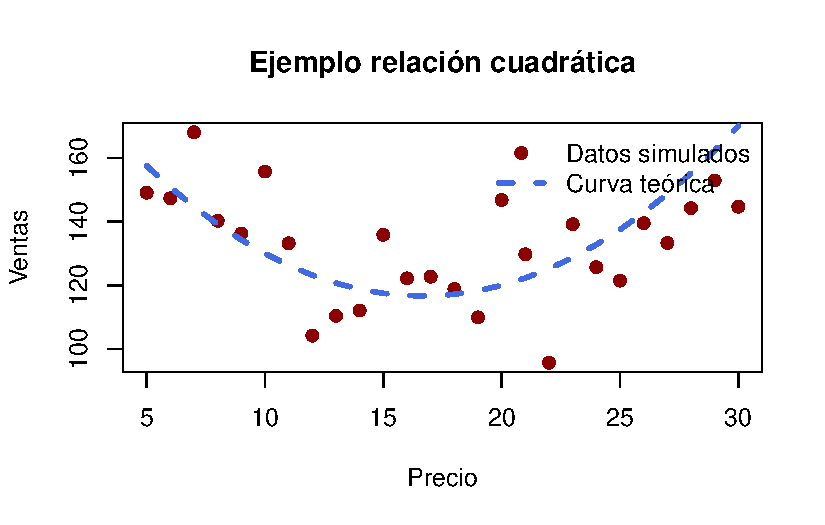
\includegraphics[keepaspectratio]{capitulo7_files/figure-pdf/grafico-cuadratico-1.pdf}}

}

\caption{Relación cuadrática entre precio y ventas (ejemplo simulado)}

\end{figure}%

\bookmarksetup{startatroot}

\chapter{Modelos de probabilidad}\label{modelos-de-probabilidad}

Hasta ahora hemos trabajado con regresiones en las que la variable
dependiente es continua: ventas, gasto promedio, calificaciones de
clientes. Pero en la práctica, muchas decisiones importantes se expresan
como un \textbf{sí o no}:

\begin{itemize}
\tightlist
\item
  ¿El cliente regresará al restaurante la próxima semana?\\
\item
  ¿El nuevo plato es un éxito (se vende) o un fracaso (no se vende)?\\
\item
  ¿El cliente recomienda el restaurante a un amigo o no?
\end{itemize}

Estas situaciones se modelan con \textbf{variables binarias}: toman el
valor 1 cuando el evento ocurre y 0 cuando no.

En este capítulo introducimos modelos donde la variable respuesta es una
\textbf{probabilidad} o una \textbf{categoría}, en lugar de una cantidad
continua.

\section{El primer intento: Modelo de Probabilidad Lineal
(MPL)}\label{el-primer-intento-modelo-de-probabilidad-lineal-mpl}

Podemos intentar usar regresión lineal directamente, tratando la
variable binaria como si fuera continua. El modelo se vería así:

\[
Pr(\text{Regresa}=1) = b_0 + b_1 \times Precio + b_2 \times Publicidad + \varepsilon
\]

Aquí:

\begin{itemize}
\tightlist
\item
  \(b_1\) indica cómo cambia la \textbf{probabilidad} de regreso cuando
  aumenta el precio en 1 unidad.\\
\item
  \(b_2\) mide el efecto de invertir más en publicidad.
\end{itemize}

\textbf{Ejemplo en el restaurante:}\\
- Cada \$1 adicional en el precio del menú disminuye la probabilidad de
regreso en 3 puntos porcentuales.\\
- Cada \$100 en publicidad aumenta la probabilidad en 2 puntos
porcentuales.

\begin{tcolorbox}[enhanced jigsaw, toptitle=1mm, opacitybacktitle=0.6, leftrule=.75mm, arc=.35mm, title=\textcolor{quarto-callout-warning-color}{\faExclamationTriangle}\hspace{0.5em}{Advertencia}, colback=white, bottomrule=.15mm, colbacktitle=quarto-callout-warning-color!10!white, opacityback=0, bottomtitle=1mm, breakable, rightrule=.15mm, coltitle=black, left=2mm, titlerule=0mm, colframe=quarto-callout-warning-color-frame, toprule=.15mm]

\textbf{Problema:} este modelo puede predecir probabilidades menores a 0
o mayores a 1, lo cual no tiene sentido.

\end{tcolorbox}

\section{La solución: Regresión
Logística}\label{la-soluciuxf3n-regresiuxf3n-loguxedstica}

Para asegurarnos de que las probabilidades siempre estén entre 0 y 1,
usamos una transformación llamada \textbf{función logística}:

\[
Pr(\text{Regresa}=1) = \frac{1}{1 + e^{-(b_0 + b_1 \times Precio + b_2 \times Publicidad)}}
\]

\begin{itemize}
\tightlist
\item
  Sin importar los valores de Precio o Publicidad, el resultado siempre
  es una probabilidad válida.\\
\item
  La relación entre las variables y la probabilidad no es lineal, sino
  en forma de ``S'': los cambios tienen más impacto en ciertos rangos y
  menos en otros.
\end{itemize}

\section{Intuición con el restaurante
🍽️}\label{intuiciuxf3n-con-el-restaurante}

Supongamos que estimamos el siguiente modelo:

\[
Pr(\text{Regresa}=1) = \frac{1}{1 + e^{-(2 - 0.05 \times Precio + 0.01 \times Publicidad)}}
\]

Interpretación:\\
- Cada \$1 más en el precio reduce la probabilidad de regreso en
aproximadamente 5\%.\\
- Cada \$100 invertidos en publicidad aumentan la probabilidad en 1\%.

Ejemplos:\\
- Menú a \$20 y publicidad de \$500 → probabilidad de regreso = 70\%.\\
- Menú a \$30 y misma publicidad → probabilidad de regreso = 55\%.

\begin{figure}[H]

{\centering \pandocbounded{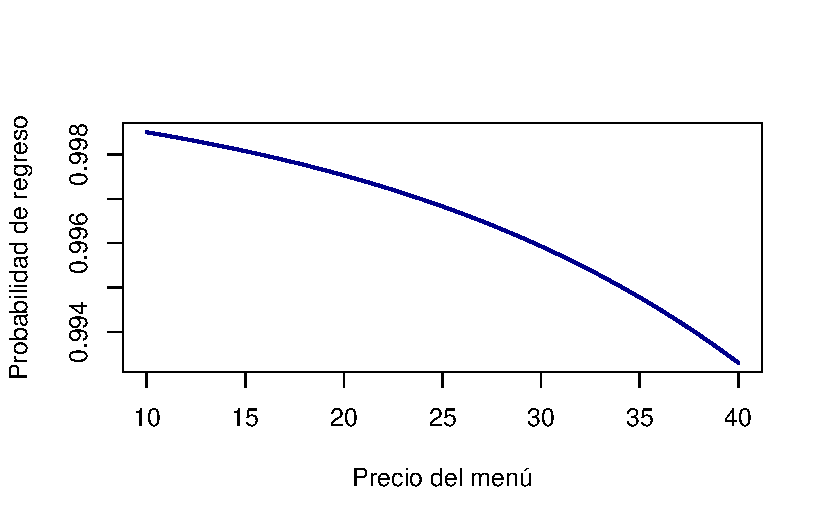
\includegraphics[keepaspectratio]{capitulo8_files/figure-pdf/ejemplo-logit-1.pdf}}

}

\caption{Curva logística: probabilidad de que un cliente regrese según
el precio}

\end{figure}%

\section{¿Cuándo usar el Modelo de Probabilidad Lineal (MPL) y cuándo la
Regresión
Logística?}\label{cuuxe1ndo-usar-el-modelo-de-probabilidad-lineal-mpl-y-cuuxe1ndo-la-regresiuxf3n-loguxedstica}

Breve respuesta intuitiva:

\begin{itemize}
\tightlist
\item
  Usa el MPL para exploraciones rápidas o cuando quieras una lectura
  lineal sencilla de los datos. Es fácil de estimar y explicar. Sirve
  mejor para efectos generales.
\item
  Usa la regresión logística cuando necesites predicciones de
  probabilidad coherentes (siempre entre 0 y 1) para cada individuo, o
  cuando la relación entre las variables y la probabilidad tenga
  curvatura (forma de ``S'').
\end{itemize}

Más en detalle:

\begin{itemize}
\tightlist
\item
  ¿Por qué el MPL puede funcionar como primer paso?

  \begin{itemize}
  \tightlist
  \item
    Es un modelo lineal simple: el coeficiente se interpreta
    directamente como ``cambio en la probabilidad (puntos porcentuales)
    por unidad''.
  \item
    Es útil para explorar señales en los datos y para comunicación
    rápida cuando las predicciones quedan mayoritariamente dentro de
    0--1.
  \end{itemize}
\item
  ¿Por qué puede fallar el MPL?

  \begin{itemize}
  \tightlist
  \item
    Puede predecir probabilidades menores que 0 o mayores que 1.
  \item
    No captura la naturaleza no lineal típica de muchas probabilidades
    (efectos que se saturan).
  \item
    Sus errores estándar pueden ser incorrectos por la
    heterocedasticidad inherente a variables binarias.
  \end{itemize}
\item
  ¿Por qué la regresión logística suele ser mejor?

  \begin{itemize}
  \tightlist
  \item
    La transformación logística garantiza probabilidades en {[}0,1{]}.
  \item
    Modela la curvatura (efectos más fuertes en ciertas zonas y más
    débiles en los extremos).
  \item
    Es el estándar práctico cuando se requiere rigor en predicción y en
    inferencia para variables binarias.
  \end{itemize}
\end{itemize}

\emph{Regla práctica:}

\begin{itemize}
\tightlist
\item
  Si necesitas rapidez y las probabilidades estimadas caen dentro de
  0.1--0.9 sin comportamientos extraños, el MPL puede servir para
  explorar. Pero si necesitas predicciones confiables, interpretación
  robusta y valores fuera del rango son posibles, usa logística.
\end{itemize}

\section{Interpretación: coeficientes, log-odds y efectos marginales
(explicado
fácil)}\label{interpretaciuxf3n-coeficientes-log-odds-y-efectos-marginales-explicado-fuxe1cil}

Lo esencial de forma muy simple:

\begin{itemize}
\tightlist
\item
  En regresión lineal un coeficiente \(β_j\) se lee directo: un aumento
  de 1 en \(X_j\) cambia la probabilidad en \(β_j\) puntos porcentuales.
\item
  En regresión logística NO se lee así. Los coeficientes actúan sobre
  los \emph{log-odds} (el logaritmo de las odds), no sobre la
  probabilidad directa.
\end{itemize}

¿Qué quiere decir eso en palabras? - Piensa que la regresión logística
primero calcula una ``puntuación'' \((x \times β)\). Esa puntuación se
transforma con la función logística para producir una probabilidad entre
0 y 1. El coeficiente \(β_j\) dice cuánto cambia la puntuación (el
log-odds), pero ese cambio no se traduce siempre en la misma variación
de probabilidad: depende del punto donde estés.

Efectos marginales --- la forma práctica de leer resultados:

\begin{itemize}
\item
  Para saber cuánto cambia la probabilidad cuando \(X_j\) aumenta en 1
  unidad necesitamos calcular el \emph{efecto marginal}, que combina
  \(β_j\) con la probabilidad actual p:

  cambio en probabilidad ≈ \[ β_j × p × (1 - p)\]

  \begin{itemize}
  \tightlist
  \item
    Observa que p(1-p) es máximo cuando p ≈ 0.5, y pequeño cuando p está
    cerca de 0 o 1. Esto significa que un mismo \(β_j\) puede implicar
    cambios grandes en la probabilidad si estamos en la zona media, y
    cambios pequeños si estamos en los extremos.
  \end{itemize}
\end{itemize}

Ejemplo muy concreto: - Si \(β_precio = -0.05\) y para un cliente
\(p = 0.5\), el efecto aproximado de subir 1 unidad el precio es:

\(-0.05 × 0.5 × 0.5 = -0.0125\) → una reducción de \(~1.25\) puntos
porcentuales en la probabilidad de regreso en ese punto.

Cómo reportarlo en práctica:

\begin{itemize}
\tightlist
\item
  Efecto marginal en la media (MEM): calcula \(p\) en las medias de las
  covariables y aplica la fórmula. Fácil de explicar.
\item
  Efecto marginal promedio (AME): calcula el efecto marginal por
  observación y promedia; refleja el efecto medio en la muestra.
\item
  Cambio discreto para variables dummy: calcula la diferencia en la
  probabilidad predicha al pasar la variable de 0 a 1.
\end{itemize}

Otra forma común: odds y odds ratio (explicado fácil)

Cuando se estima un modelo binomial (logístico) los coeficientes se
obtienen en la escala de los \emph{log-odds}. Para pasar a una
interpretación más intuitiva aplicamos la exponencial de ese
coeficiente:

\begin{itemize}
\tightlist
\item
  OR = \(exp(β_j)\)
\end{itemize}

Esto se denomina \emph{odds ratio} (OR) y compara cómo cambian las odds
cuando una variable aumenta en una unidad.

Definiciones claras e intuitivas:

\begin{itemize}
\item
  Odds: la razón entre la probabilidad de éxito y la probabilidad de
  fracaso.

  odds = \(p / (1 - p)\)

  donde \(p\) es la probabilidad de que ocurra el evento de interés.
\item
  Odds ratio (OR): la razón entre las odds en dos grupos o condiciones.

  OR = odds en el grupo A / odds en el grupo B

  Si OR \textgreater{} 1, las odds son mayores en el numerador; si OR
  \textless{} 1, las odds son menores.
\end{itemize}

Ejemplo simple e intuitivo:

\begin{itemize}
\tightlist
\item
  Si \(exp(β_precio) = 0.95\), eso significa que aumentar el precio en 1
  unidad multiplica las odds por \(0.95\) (una reducción del 5\% en las
  odds). No es exactamente la misma reducción en la probabilidad, pero
  da una idea clara de dirección y magnitud relativa.
\end{itemize}

Consejo práctico para comunicar resultados:

\begin{itemize}
\tightlist
\item
  Usa OR cuando quieras mostrar «cuánto cambian las odds» (útil en
  reportes) y complementa siempre con efectos marginales o cambios en
  probabilidades para audiencias no técnicas.
\end{itemize}

Resumen para el lector final:

\begin{itemize}
\tightlist
\item
  MPL: simple y útil para exploración, pero con límites (probabilidades
  fuera de rango, errores en inferencia).
\item
  Logística: un poco más compleja de interpretar, pero produce
  probabilidades coherentes; siempre traduzcas β a efectos marginales o
  a cambios en probabilidad para comunicar resultados a audiencias no
  técnicas.
\end{itemize}




\end{document}
